%%%%%%%%%%%%%%%%%%%%
% CHAPTER 2
% %%%%%%%%%%%%%%%%%%
\chapter{Group Theory}
\begin{quote}
    \textit{Wit lies in recognizing the resemblance among things which differ and the difference between things which are alike.}\\

Madame de Stael
\end{quote}
\section{Definition of a Group}
\begin{definition}[Group]
A non-empty set $G$ with a binary operation $\ \cdot \ $ (commonly called ``dot") is a \textit{group} if 4 properties are satisfied:
\begin{enumerate}
    \item $a,b\in G \implies a\cdot b \in G$ (Closure)
    \item $a,b,c\in G\implies a\cdot(b\cdot c)=(a\cdot b)\cdot c$ (Associativity)
    \item $\exists \ e \in G\ni a\cdot e=e\cdot a=a \ \forall a \in G$ (Existence of Identity)
    \item $\forall \ a\in G, \exists \ a^{-1}\in G\ni a\cdot a^{-1}=a^{-1}\cdot a = e$ (Existence of Inverses under $\cdot$)
\end{enumerate}
\end{definition}

%So if someone tells you they have a group they are working with. There are some things you can demand of them to verify they indeed have a group on their hands. They must show you the non-empty set and binary operation that they are considering. And they most show you that this set under the specified operation obeys the 4 properties of a group.


% \textbf{Defn:} A non-empty set $G$ with a binary operation $\ \cdot \ $ (commonly called ``dot") is a group if 4 properties are satisfied:
% \begin{enumerate}
%     \item $a,b\in G \implies a\cdot b \in G$ (Closure)
%     \item $a,b,c\in C\implies a\cdot(b\cdot c)=(a\cdot b)\cdot c$ (Associativity)
%     \item $\exists \ e \in G\ni a\cdot e=e\cdot a=a \ \forall a \in G$ (Existence of Identity)
%     \item $\forall \ a\in G, \exists \ a^{-1}\in G\ni a\cdot a^{-1}=a^{-1}\cdot a = e$ (Existence of Inverses under $\cdot$)
% \end{enumerate}
\begin{example}
Let $G=\Z$ and take $\cdot$ to be ordinary integer addition. In this group, $e=0$ and $\forall a \in \Z, a^{-1}=-a$.
\end{example}
%\textbf{Example:} Let $G=\Z$ and take $\cdot$ to be ordinary integer addition. In this group, $e=0$ and $\forall a \in \Z, a^{-1}=-a$.\steezybreak\\
\begin{definition}[Abelian Group]
$G$ is \textit{abelian} if $\forall a,b\in G, a\cdot b= b\cdot a$.
\end{definition}
\begin{definition}[Order of a Group]
The \textit{order} of $G$, denoted $o(G)$ is the number of elements in $G$. \\ If $o(G)$ is finite, $G$ is known as a \textit{finite group}, otherwise $G$ is an \textit{infinite group}.
\end{definition}
\href{https://en.wikipedia.org/wiki/Niels_Henrik_Abel}{Abelian groups are named after Norwegian Mathematician Niels Henrik Abel.}
\section{Examples of some Groups:} 
\begin{enumerate}
    \item $\Z$ is an infinite abelian group under $+$.
    \item $\R$ is an infinite abelian group under $+$.
    \item If we let $G=\Z$ and take $\cdot$ to be integer multiplication we can see that properties 1-3 hold but property 4 fails:
    \begin{enumerate}[label=\roman*]
        \item Closure $\checkmark$ (multiplying two integers together always gives you another integer)
        \item Associative $\checkmark$, Integer Mult. is associative
        \item Existence of identity $\checkmark$, 1 serves this purpose under multiplication
        \item Existence of inverse $X$!! $\Z$ is not a group under integer multiplication because $n\cdot (\frac{1}{n})=1$ but $\frac{1}{n}$ is not necessarily an element of $\Z$!
    \end{enumerate}
    $\therefore$ $\Z$ under integer multiplication is NOT a group.
    \item How about if we try $G=\R$ with $\cdot$ as real number multiplication? This is still not a group because 0 has no multiplicative inverse in $\R$. 
    \item $\R-\{0\}$ (i.e. the real numbers minus [without] element $\{0\}$) under multiplication is an infinite abelian group.
    \item $G=\Z_n$ under the operation defined by $[a]+[b]=[a+b]$ is a finite abelian group of order $n$.
\end{enumerate}
\subsection{The Cayley Table}
For this discussion we will consider the group $\Z_4=\{[0],[1],[2],[3]\}=\{4\Z,4\Z+1,4\Z+2,4\Z+3\}$. \steezybreak\\
\noindent The ``Cayley Table" displays all possible ``products" of $a\cdot b=ab$ for $a,b\in G$. A simple example of \textit{how} to compute the entries of the Cayley table for an arbitrary group of order 4 is given below in Table \ref{tab:Cayley_dummy}. It should be noted that a proper Cayley table will represent the products in their simplest form, i.e. as one of the elements $e,a,b,...$ listed along the top or left side of the table. We demonstrate this in the next table for $\Z_4$, Table \ref{tab:Cayley_Z4}, where rather than writing $[1]\cdot [0]$ or $[2]\cdot [2]$ we instead write the result of the ``product" itself, i.e. the elements $[1]$ and $[0]$ respectively.
\begin{table}[h!]
    \centering
    \begin{tabular}{c||c|c|c|c|}
         $\bsfrac{b\text{ (right)}}{a\text{ (left)}}$& e&a&b&c  \\ \hline \hline
         e&$e\cdot e$&$e\cdot a$&$e\cdot b$&$e\cdot c$  \\ \hline
         a&$a\cdot e$&$a\cdot a$&$a\cdot b$&$a\cdot c$  \\ \hline
         b&$b\cdot e$&$b\cdot a$&$b\cdot b$&$b\cdot c$  \\ \hline
         c&$c\cdot e$&$c\cdot a$&$c\cdot b$&$c\cdot c$ \\ \hline
    \end{tabular}
    \caption{Cayley Table for group $(G,\cdot)$ where $o(G)=4$ and $G=\{e,a,b,c\}$}
    \label{tab:Cayley_dummy}
\end{table}
\begin{table}[h!]
    \centering
    \begin{tabular}{c||c|c|c|c|}
         $\bsfrac{b\text{ (right)}}{a\text{ (left)}}$& [0]&[1]&[2]&[3]  \\ \hline \hline
         [0]&[0]&[1]&[2]&[3]  \\ \hline
         [1]&[1]&[2]&[3]&[0]  \\ \hline
         [2]&[2]&[3]&[0]&[1]  \\ \hline
         [3]&[3]&[0]&[1]&[2] \\ \hline
    \end{tabular}
    \caption{Cayley Table for $\Z_4$}
    \label{tab:Cayley_Z4}
\end{table}

Using this table we can confirm again for ourselves that $\Z_4$ is a group under the defined addition. 1) Closure holds since all products are in $\Z_4$, 2) associativity holds because $\Z$ is associative under $+$, 3) $e$ is $[0]$ here (see first row and column of table), furthermore 4) each class has an inverse (check the table for the products that go to $[0]$, every element has an inverse under the binary operation ``$\cdot$"). \href{https://en.wikipedia.org/wiki/Arthur_Cayley}{Cayley tables are named after British Mathematician Arthur Cayley.}\\
\newpage
\noindent\textbf{Characteristics of the Cayley Table:}
\begin{enumerate}
    \item Every row or column of the table is a permutation of the group elements.\\
    \textit{Proof:} Suppose $b,c\in G$ are distinct elements (i.e. $b\neq c$) corresponding to two distinct rows (columns) of the table, then if there is a repeat in a row (a column), then for some $a\in G$ we have that $a\cdot b=d$ and $a\cdot c=d$, then $ab=ac$. Since $G$ is a group and $a\in G \implies \exists a^{-1}\in G $, so
    \begin{align}
        a^{-1}\cdot (ab)&=a^{-1}\cdot (ac) \nonumber \\
        (a^{-1}\cdot a)\cdot b&=(a^{-1}\cdot a)\cdot c \nonumber \\
        e\cdot b&=e\cdot c \nonumber \\
        \iff b&=c \ \ \Rightarrow\Leftarrow \ \ \ \ \ \ \ \ \blacksquare \nonumber
    \end{align}
    \item ``$e$" in the body of the table indicates elements that are inverses of each other. This is easy to prove since $b\cdot a= e \implies b=a^{-1}, a=b^{-1} $
    \item \begin{align}
        G \text{ abelian } &\iff ab=ba \ \forall \ \ a,b \in G \nonumber \\
        &\iff (i^{th} \text{ row}, j^{th} \text{ col}) \text{ entry of Cayley table } = (j^{th} \text{ row}, i^{th} \text{ col}) \text{ entry of Cayley table } \nonumber \\
        &\iff \text{Table has symmetry down the main diagonal} \nonumber
    \end{align}
\end{enumerate}

\noindent\textbf{Some more Examples of Groups}

\begin{enumerate}
\setcounter{enumi}{6}
    \item $GL_2(\R)=\{\text{invertible } 2\times 2 \text{ matrices with entries in } \R\}$, Matrix $M$ is invertible $\iff  \ \det(M)\neq 0$ (This is a linear algebra fact that is proven in any standard LA course, take as a given); if $M= 	\left(\begin{matrix}
a & b \\
c & d 
\end{matrix}\right) \text{ then } \det(M)=ad-bc$. Under the operation ``$\cdot$" of matrix multiplication, $GL_2(\R)$ is an infinite non-abelian group. This group is called `` general linear group of degree 2 with real entries". Let's prove it's a non-abelian infinite group, we will start by showing it is infinite and non-abelian under the suggested ``$\cdot$" (matrix multiplication), and then we will proceed to show it satisfies the 4 properties of a group. Note, below $\Z^+ = \{n\in \Z| n>0\}$, denotes the positive integers (does not include 0)\steezybreak\\
\end{enumerate}
\noindent \textit{Proof:} $\forall n \in \Z^+, \left(\begin{matrix}
n & 0 \\
0 & n 
\end{matrix}\right) \in GL_2(\R)$, so $GL_2(\R)$ is infinite. Now if we consider some elements from $GL_2(\R)$ we can immediately see $GL_2(\R)$ is non-abelian:\\
\begin{align}
    A &= \left(\begin{matrix}
2 & 0 \\
0 & 1 
\end{matrix}\right) \in GL_2(\R) \nonumber \\
B &= \left(\begin{matrix}
1 & 0 \\
2 & 1 
\end{matrix}\right) \in GL_2(\R) \nonumber \\
A\cdot B &\neq B\cdot A \nonumber \\
&\therefore GL_2(\R) \text{ is not abelian.} \nonumber
\end{align}
So, it has infinite elements and does not have the abelian property under the operation, but is it a group? Let's show the four required properties: Closure, Associativity under the operation, Existence of an identity element, and existence of inverses under the operation:
\begin{enumerate}[label=(\roman*)]
    \item \textit{Closure:} Take $A,B\in GL_2(\R)$, now $A\cdot B=AB$ is the product of a $2\times 2$ with a $2\times 2$, and in general when we multiply a $m\times n$ matrix by a $n\times p$ matrix, we get a $m\times p$ matrix (i.e. we always line up the left matrix's column dimension with the row dimension of the right matrix) so the product of two $2\times 2$ matrices will itself be a $2\times 2$ matrix. Is it invertible? To show this we will use another very common and easy to prove linear algebra fact, namely that for square matrices $A,B \in \R^{n\times n}$ it is always true that $\det(AB)=\det(A)\det(B)$. Since $A,B\in GL_2(\R) \implies \det(A)\neq 0 \text{ and } \det(B)\neq 0 \implies \det(AB)=\det(A)\det(B)\neq 0$. So the product, $AB$ of two invertible matrices $A,B$ is itself invertible and we have $AB\in GL_2(\R)$. \\ $\therefore GL_2(\R)$ is closed under matrix multiplication.
    \item \textit{Associativity: } Matrix multiplication is associative (Linear Algebra Fact, we will treat this as a given as well since this isn't a Linear Algebra class, though this should be easy enough to prove yourself using the dot product representation of matrix multiplication!)
    \item \textit{Identity: }There exists an identity $e$ for this set under matrix multiplication:
    \begin{align}
        e&=\left(\begin{matrix}
1 & 0 \\
0 & 1 
\end{matrix}\right) = I_2\nonumber 
    \end{align}
    Because for all $A\in GL_2(\R)$ we have $A\cdot I_2=I_2\cdot A = A$.
    \item \textit{Existence of Inverses: }$\forall A \in GL_(\R)$, $A$ is invertible so $\exists A^{-1}$, is $A^{-1}\in GL_2(\R)$? Well, $A^{-1}$ is a $2\times 2$ with real entries, we will use one last linear algebra fact: For invertible square matrices $A\in \R^{n\times n}$, $\det(A^{-1})=(\det(A))^{-1}=\frac{1}{\det(A)}$, applying this fact to our hypothesis we can see $det(A^{-1})=\frac{1}{\det(A)}\neq 0$, so $A^{-1}\in GL_2(\R). \ \ \ \ \ \ \ \blacksquare$
\end{enumerate}\steezybreak
\noindent\textbf{Examples of Groups (cont'd)}
\noindent\begin{enumerate}
\setcounter{enumi}{7}
    \item Suppose $S$ is a set with $n$ elements. The following $(G,\cdot)$ defines a group:
    \begin{align}
        &G= \{\text{ bijections of } S \text{ onto } S\} = S_n \nonumber \\
        &\cdot \text{ is composition of maps } (\circ) \nonumber
    \end{align}
\end{enumerate}
\textit{Proof:}
\begin{enumerate}[label=(\roman*)]
    \item \textit{Closure: } $\sigma, \tau \in S_n \implies \tau \circ \sigma \in S_n$ by Lemma 1.2.2.
    \item \textit{Associativity: } Lemma 1.2.1
    \item \textit{Identity: } $e$ in this group is the identity map $I_S$
    \item \textit{Inverses: } By Lemma 1.2.3 we have that $\forall \sigma \in S_n,  \exists \sigma^{-1}\in S_n \ni \sigma\circ\sigma^{-1}=\sigma^{-1}\circ\sigma=I_S$
\end{enumerate}
$\therefore S_n$ is a group under $\circ$.\steezybreak\\
\noindent $S_n$ is called the symmetric group of degree $n$. Alternate notation for this group is $A(S)$ `` Automorphisms of $S$ " this notation is sometimes used for finite $S$ and \textit{always} used for infinite $S$.

\subsection{An Example with $S_3$:} Construct the Cayley Table for $S_3$.
\begin{figure}[ht!]
    \centering
    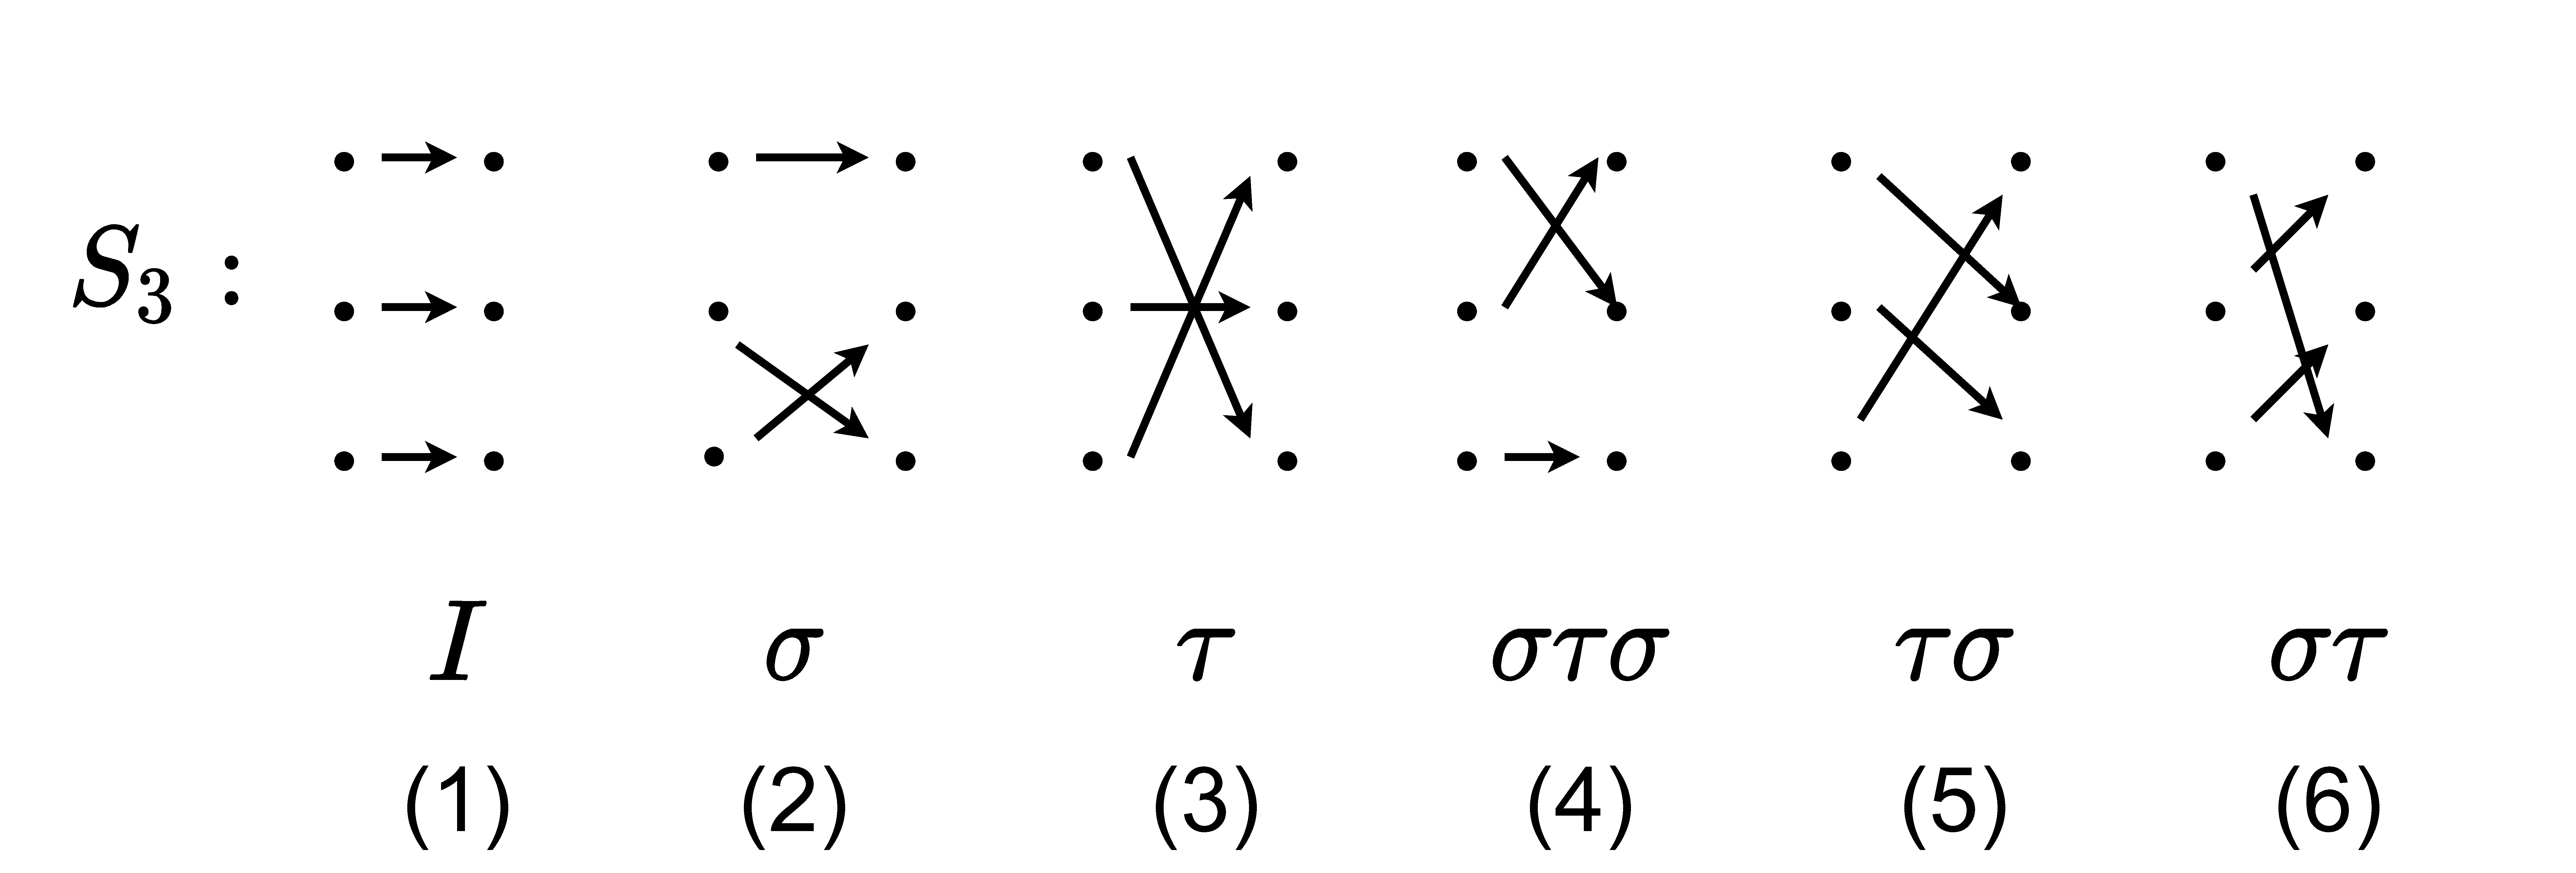
\includegraphics[width=0.8\textwidth]{Figures/S_3 Group Example.pdf}
    \caption{Elements of $S_3$: $S_3$'s group elements correspond to bijective (invertible) mappings from a set of three elements back to itself}
    \label{fig:S3elts}
\end{figure}
\begin{table}[h!]
    \centering
    \begin{tabular}{c||c|c|c|c|c|c|}
         $\bsfrac{b\text{ (right)}}{a\text{ (left)}}$& $I$&$\sigma$&$\tau$&$\sigma\tau$&$\tau\sigma$&$\sigma\tau\sigma$  \\ \hline \hline
         $I$&$I$&$\sigma$&$\tau$&$\sigma\tau$&$\tau\sigma$&$\sigma\tau\sigma$  \\ \hline
         $\sigma$&$\sigma$&$I$&$\sigma\tau$&$\tau$&$\sigma\tau\sigma$& $\tau\sigma$\\ \hline
         $\tau$&$\tau$&$\tau\sigma$&$I$&$\sigma\tau\sigma$ &$\sigma$ &$\sigma\tau$  \\ \hline
         $\sigma\tau$&$\sigma\tau$& $\sigma\tau\sigma$&... & & &$\vdots$ \\ \hline
         $\tau\sigma$ & $\tau \sigma$ &... & & & &   \\ \hline
         $\sigma\tau\sigma$ & $\sigma\tau\sigma$ &... & & & &   \\ \hline
    \end{tabular}
    \caption{Cayley Table for group $S_3$}
    \label{tab:Cayley_S3}
\end{table}
Note that because $\tau\sigma\neq \sigma \tau$ we have a non-abelian group. \steezybreak\\
\noindent The diagram in Figure \ref{fig:S3elts} shows the various bijections that make up the elements of $S_3$, using these mappings we can see some basic facts just by following the points through the composed mappings:
\begin{align}
    \sigma^2&= I \nonumber \\
    \tau^2&=I \nonumber \\
    \sigma\tau\sigma&=\tau\sigma\tau \nonumber
\end{align}
So,
\begin{align}
    \sigma\tau\sigma \circ \tau\sigma = \sigma(\tau\sigma\tau)\sigma= \sigma(\sigma\tau\sigma)\sigma=\sigma^2\tau\sigma^2=I\tau I=\tau \nonumber 
\end{align}
With these facts observed you should be able to fill in the rest of the Cayley table!\steezybreak\\
Now that we have gotten our feet wet with some groups and some ideas relating to their structure, we will prove some elementary facts that hold for all groups. Remember a group is defined by a set $G$ and a group operation $\cdot$ and it obeys four properties.\vspace{-0.5cm}
\section{Some Elementary Results:} 
\begin{lemma}[Elementary Results with Groups]
If $G$ is a group with operation ``$\cdot$", then
\begin{enumerate}[label=\alph*)]
    \item The Identity Element of $G$ is \textit{unique}.
    \item Every elt. in $G$ has a \textit{unique} inverse in $G$
    \item $\forall a \in G$, $(a^{-1})^{-1}=a$
    \item $\forall a,b \in G$, $(ab)^{-1}=b^{-1}a^{-1}$
\end{enumerate}
\textit{Proof:}
\begin{enumerate}[label=\alph*)]
    \item Suppose $e$ and $f$ are both identity elements in $G$, then $f=e\cdot f=e$ (first equality because $e$ is an identity, second equality because $f$ is). $\therefore f=e$ (they are the same).
    \item Suppose $a\in G$ has two inverses $x,y \in G$. Then
    \begin{align}
        x=e\cdot x=(y\cdot a)\cdot x = y\cdot(a\cdot x)=y\cdot e=y\nonumber
    \end{align}
    $\therefore $ inverses $x,y$ are the same elt. (i.e. the inverse of $a$ is unique).\\ 
    \noindent NOTE: part b guarantees if $xy=e$ then you automatically get $yx=e$ since
    \begin{align}
        xy&=e \nonumber \\
        &\implies y\cdot (xy)\cdot y^{-1} = yey^{-1} \nonumber \\
        &\implies yx(y\cdot y^{-1})= yy^{-1} \nonumber \\
        &\implies yxe=e \nonumber \\
        &\implies yx=e \nonumber
    \end{align}
    \item $\forall \ a \in G, (a^{-1})^{-1}=a:$ Take arbitrary $a\in G$, then $a\cdot a^{-1}=e$ and $a^{-1}\cdot a= e$, This set of equations shows that $a$ is the inverse of $a^{-1}$, $\therefore (a^{-1})^{-1}=a$.
    \item $(ab)^{-1}=b^{-1}a^{-1}:$ For all $a,b\in G$ we know $ab\in G$ by closure of group $G$ and furthermore, $ab$ must have a \textit{unique} inverse in $G$, so if $b^{-1}a^{-1}$ satisfies the properties of an inverse for $ab$ then $b^{-1}a^{-1}$ \textbf{is} $(ab)^{-1}$:
    \begin{align}
        (b^{-1}a^{-1})ab= b^{-1}(a^{-1}a)b=b^{-1}eb=b^{-1}b=e \nonumber
    \end{align}
    $\therefore b^{-1}a^{-1} \textit{ is the inverse of } ab; \ \ (ab)^{-1}=b^{-1}a^{-1} \ \ \ \ \ \ \ \blacksquare$
\end{enumerate}
\end{lemma}

\begin{tcolorbox}
\begin{center}
    $\star\star\star$ \textbf{Read up to this point to Complete Homework 2} $\star\star\star$
\end{center}
\end{tcolorbox}
\newpage
\subsection{Laws of Exponents for Groups } This subsection could very well be titled ``Creating new and consistent notation for applying the group operation to a single element with itself many times" because that is what we will be doing here. By unlocking this new notation, that is consistent with our notion of a group, we will be able to prove more nuanced facts with a compact notation.\steezybreak
\begin{definition}[Exponents for Groups]
\noindent $G$ a group, $a\in G$, and $k\in \Z^+$. \\
Exponents on group elements are defined as follows:
\begin{align}
    a^{0} & \eqdef e \nonumber \\
    a^{k} &= a\cdot a\cdot a \cdot ... \cdot a \ (  k \text{ times} )\nonumber \\
    a^{-k} &= a^{-1}\cdot a^{-1} \cdot a^{-1} \cdot ... \cdot a^{-1} \ \ ( k \text{ times}) = (a^{-1})^k\ \  \underset{\star\star}{=} (a^{k})^{-1} \nonumber
\end{align}
\textit{Proof of $\star\star$:} we wish to show that $a^{-k}=(a^{k})^{-1}$ 
\begin{align}
    (a^k)^{-1}=(a\cdot a\cdot a \cdot ... \cdot a)^{-1} = a^{-1}\cdot a^{-1}\cdot a^{-1} \cdot ... \cdot a^{-1}\nonumber 
\end{align}
Where the last equality is established by repeatedly applying part (d) of Lemma 2.3.1. \steezybreak\\
Note also: any power of $e$ is $e$, i.e. $e^{-k}=(e^{-1})^k=e$
\end{definition}

\begin{proposition}[Law of Exponents]
If $G$ is a group, $a\in G, m,n\in \Z$, then 
\begin{align}
    a^m a^n&=a^{m+n} \nonumber \\
    (a^m)^n&= a^{mn} \nonumber
\end{align}
\textit{Proof:} This proof will consider all of the cases for a pair $m,n\in \Z$ and we will show the laws hold for each case.
\begin{enumerate}[label=Case \arabic*:]
    \item $m=0,n=0$, then $m+n=0$ and $mn=0$ and we see:
    \begin{align}
        a^ma^n&=a^0a^0=e\cdot e=e=a^0=a^{m+n} \nonumber \\
        (a^m)^n&=(a^0)^0=e^0=e=a^0=a^{mn} \nonumber
    \end{align}
    \item $m=0, n\neq 0$
    \begin{align}
        a^ma^n&=a^0a^n=e\cdot a^n=a^n=a^{0+n}=a^{m+n} \nonumber \\
        (a^m)^n&=(a^0)^n=e^n=e=a^0=a^{0n}=a^{mn} \nonumber
    \end{align}
    \item $m\neq 0, n=0$ (Proof is Similar to Case (2), leave to students to show)
    \item Both Positive-- $m,n\in \Z^+$ (i.e. both $m$ and $n$ are positive integers)
    \begin{align}
        a^ma^n&=\underset{m\text{ times}}{(a\cdot a\cdot a \cdot ... \cdot a)}\underset{n \text{ times}}{(a\cdot a\cdot a \cdot ... \cdot a)}=a^{m+n} \nonumber \\
        (a^m)^n&=\underset{n\text{ times}}{(a^m\cdot a^m\cdot ... \cdot a^m)}=\underset{n \text{ times}}{(\underset{m }{a\cdot ... \cdot a})...(\underset{m}{a\cdot ... \cdot a})}=a^{mn}\nonumber
    \end{align}
    \item Both Negative-- $m,n\in \Z^+$ (use $-m$ and $-n$) (Note, the square brackets $[\ ]$ used to prove the second statement are normal parentheses, not equivalence class notation, this was just to make the proof read cleaner instead of having a bunch of nested round parentheses)
    \begin{align}
        a^{-m}a^{-n}& \underset{\text{by }\star\star}{=} (a^{-1})^m(a^{-1})^n \underset{\text{by Case (4)}}{=} (a^{-1})^{m+n} \underset{\text{by }\star\star}{=} a^{-(m+n)}=a^{(-m)+(-n)} \nonumber \\
        (a^{-m})^{-n} &\underset{\text{by }\star\star}{=} ((a^m)^{-1})^{-n} \underset{\text{by }\star\star}{=} [((a^m)^{-1})^{-1}]^{n} \underset{\text{Lemma 2.3.1 (c)}}{=} [a^m]^n= a^{mn}= a^{(-m)(-n)} \nonumber 
    \end{align}
    \item Pos-Neg -- $m,n\in \Z^+$ (use $m$ and $-n$)
    \begin{align}
        a^m a^{-n}&\underset{\text{by $\star$}}{=} a^m (a^{-1})^n = \underset{\text{m}}{(a\cdot ... \cdot a)}\cdot \underset{n}{(a^{-1}\cdot ... \cdot a^{-1})} \nonumber
    \end{align}
    Since $a\cdot a^{-1}=e$ we can cancel pairs from the inside out:
    \begin{align}
        &\text{if } m=n, a^m\cdot a^{-n}=e \nonumber \\
        &\text{if } m>n, a^m\cdot a^{-n} \underset{n \ a's\text{ get cancelled}}{=}a^{m-n}=a^{m+(-n)} \nonumber\\
        &\text{if } m<n, a^ma^{-n} \underset{m \ a^{-1} \text{ get cancelled}}{=} (a^{-1})^{n-m} \underset{\text{by $\star$}}{=} a^{-(n-m)}=a^{m+(-n)}\nonumber
    \end{align}
    \begin{align}
        (a^m)^{-n}\underset{\text{by $\star$}}{=} [(a^m)^{-1}]^n\underset{\text{by $\star$}}{=}[(a^{-1})^m]^n \underset{\text{case 4}}{=}(a^{-1})^{mn} \underset{\text{by $\star$}}{=}a^{-mn}=a^{m(-n)}\nonumber
    \end{align}
    \item Neg-Pos -- $m,n\in \Z^+$ (use $-m$ and $n$)\\
    \begin{align}
        a^{-m}a^{n}&\underset{\text{by $\star$}}{=}(a^{-1})^m a^n\underset{\text{Lem 2.3.1 (c)}}{=}(a^{-1})^m[(a^{-1})^{-1}]^n = (a^{-1})^m(a^{-1})^{-n}\underset{\text{by case 6}}{=} (a^{-1})^{m+(-n)} \nonumber \\
        &=(a^-1)^{m-n}= a^{-(m-n)}= a^{(-m)+n} \nonumber \\ \nonumber \\
        (a^{-m})^n&\underset{\text{by $\star$}}{=}((a^m)^{-1})^n\underset{\text{by $\star$}}{=}(a^m)^{-n}\underset{\text{case 6}}{=}a^{m(-n)}=a^{(-m)(n)} \ \ \ \ \ \ \ \ \blacksquare\nonumber
    \end{align} 
\end{enumerate}
Phew, that sure was a lot of cases, but now we can see our bases are covered and these rules for exponents are consistent with our notion of a group and its binary operation ``$\cdot$".
\end{proposition}

\begin{lemma}
$G$ is a group\\
$\forall \ \ a,b,c \in G$,
\begin{enumerate}[label=\roman*)]
    \item if $ab=ac \implies b=c$      (left-cancellation)
    \item if $ba=ca \implies b=c$      (right-cancellation)
\end{enumerate}
%\textit{Note: }These cancellation rules can be very convenient however, we must be careful about what they say and do not say. Remember that, in general, $a\cdot b \neq b\cdot a$ (this is only the case in Abelian groups).\\
\textit{Proof:} 
\begin{enumerate}[label=\roman*)]
    \item Assume $ab=ac$. $a$ is a group element $\therefore \exists \ a^{-1}\in G \ni a^{-1}\cdot a = a\cdot a^{-1}=e$. Now then if we apply this fact to our assumption we see that
    \begin{align}
        a^{-1}ab=a^{-1}ac \implies eb=ec \implies b=c\nonumber
    \end{align}
    \item Assume $ba=ca$,
    \begin{align}
        (ba)a^{-1}=(ca)a^{-1} \implies be=ce \implies b=c \ \ \ \ \ \blacksquare \nonumber
    \end{align}
\end{enumerate}
\end{lemma}
Great! 
\begin{notation}
Writing out the square brackets/boxes $[a],[b], ...$ everywhere to indicate our equivalence classes/group elements is somewhat tiresome. While we would normally denote a group like $\Z_5$ as having elements $\Z_5=\{[0],[1],[2],[3],[4]\}$; By an abuse of notation, we will henceforth describe the equivalence classes with the following more compact notation: $\Z_5=\{0,1,2,3,4\}$. That is, we will intentionally use less precise notation for convenience (so we don't have to put brackets around an equivalence class/group element every time we want to refer to it.)
\end{notation}
\begin{example}
Given $a=\left(\begin{matrix}
4 & 3 \\
0 & 7 
\end{matrix}\right)$ and $b=\left(\begin{matrix}
5 & 0 \\
6 & 7 
\end{matrix}\right)$, $a,b\in GL_2(\Z_9)=\{2\times 2 \text{ matrices with entries in }\Z_9\}$\\
$ab=\left(\begin{matrix}
4 & 3 \\
0 & 7 
\end{matrix}\right)\left(\begin{matrix}
5 & 0 \\
6 & 7 
\end{matrix}\right)\underset{\text{mult. mod 9}}{=}\left(\begin{matrix}
2 & 3 \\
6 & 4 
\end{matrix}\right)$\steezybreak\\
\end{example}
\begin{example}[Constructing a Group from Generators]
\noindent The first problem of our personal group studies (i.e. each student will be assigned a group to study over the remainder of the semester) will be to construct the Cayley table for your group. We will give an example here where we consider the group generated by $a=\left(\begin{matrix}
-1 & -1 \\
0 & 1 
\end{matrix}\right)$ and $b=\left(\begin{matrix}
0 & 1 \\
1 & 0 
\end{matrix}\right)$ under regular matrix multiplication. Under matrix multiplication, 
The approach for constructing a Cayley table from two generating elements $a$ and $b$ is as follows:
\begin{enumerate}
    \item Identify $e$ and put it in the table first
    \item Get powers of $a$
    \item Get powers of $b$
    \item Get products of $a$,$b$ etc.
\end{enumerate}
So we will begin by identifying the identity that works with our $\cdot$ and then we will look at how many unique powers of $a$ exist under the $\cdot$. Then we will do the same for $b$. Lastly we will see if we can make any more elements by multiplying a power of $a$ or $b$ from the left or right by a power of $b$ or $a$, respectively. We start by pointing out the only $2\times 2$ matrix that can work as an identity element under regular matrix multiplication (1) and then we look at how many unique powers of $a$ there are (2):
\begin{align}
    e =\left(\begin{matrix}
1 & 0 \\
0 & 1 
\end{matrix}\right)\nonumber \\
a^2=\left(\begin{matrix}
-1 & -1 \\
1 & 0 
\end{matrix}\right)\left(\begin{matrix}
-1 & -1 \\
1 & 0 
\end{matrix}\right)=\left(\begin{matrix}
0 & 1 \\
-1 & -1 
\end{matrix}\right) \nonumber \\
a^3=a^2\cdot a=\left(\begin{matrix}
1 & 0 \\
0 & 1 
\end{matrix}\right) \nonumber
\end{align}
Continuing on in this fashion let's look at the powers of $b$:
\begin{align}
    b\cdot b= b^2=\left(\begin{matrix}
0 & 1 \\
1 & 0 
\end{matrix}\right)\left(\begin{matrix}
0 & 1 \\
1 & 0 
\end{matrix}\right)=\left(\begin{matrix}
1 & 0 \\
0 & 1 
\end{matrix}\right)=e \nonumber 
\end{align}
So it looks like there is only 1 unique power of $b$, and $b$ is it's own inverse. Let's have a look at the products and see how many unique elements we can come up with in total (so far we have identified four unique elements: $e,a,a^2,b$)
\begin{align}
    a\cdot b &= \left(\begin{matrix}
-1 & -1\\
1& 0 
\end{matrix}\right)\left(\begin{matrix}
0 & 1 \\
1 & 0 
\end{matrix}\right) = \left(\begin{matrix}
-1 & -1 \\
0 & 1
\end{matrix}\right) \nonumber\\
b\cdot a &= \left(\begin{matrix}
0 & 1 \\
1 & 0 
\end{matrix}\right)\left(\begin{matrix}
-1 & -1 \\
1 & 0 
\end{matrix}\right) =\left(\begin{matrix}
1 & 0 \\
-1 & -1 
\end{matrix}\right) = a^2b \ \ \ \ \ \ \text{ (confirm for yourself)} \nonumber \\
b\cdot a^2&= (a^2)^2 b \ \ \ \ \ \ \ \ \ \ \ \ \ \ \ \ \ \ \ \ \ \ \ \ \ \ \ \ \ \ \ \ \ \text{ (confirm for yourself)} \nonumber \\
ba^2b&= (a^2)^2b^2=a\cdot a^3=a \nonumber
\end{align}
From here it should be clear that if we take the product of any one of these elements from the left or right by any other one of the elements we have already discovered, we will just get another element that we have already discovered, i.e., we have identified all of the unique elements. To prove this in the most explicit way possible, we form \textit{each} of those products as the entries of the Cayley table. Let's give each of them a simple name (notice, we named the elements in terms of the powers of the generator elements $a$, $b$ and products of $a$ and $b$) and collect our simplified products (simplified using the relations we discovered above such as $a^3=b^2=e$ and $b\cdot a^2=a\cdot b$) in a Cayley Table.
\begin{table}[ht!]
    \centering
    \begin{tabular}{c||c|c|c|c|c|c|}
         $\bsfrac{b\text{ (right)}}{a\text{ (left)}}$& $e$&$a$&$a^2$&$b$&$ab$&$a^2b$  \\ \hline \hline
         $e$&$e$&$a$&$a^2$&$b$&$ab$&$a^2b$  \\ \hline
         $a$&$a$&$a^2$&$e$&$ab$&$a^2b$& $b$\\ \hline
         $a^2$&$a^2$&$e$&$a$&$a^2b$ &$b$ &$ab$  \\ \hline
         $b$&$b$& $a^2b$&$ab$ &$e$ &$a^2$ &$a$ \\ \hline
         $ab$ & $ab$ &$b$ &$a^2b$ &$a$ &$e$ &$a^2$   \\ \hline
         $a^2b$ & $a^2b$ & $ab$ &$b$ &$a^2$ &$a$ &$e$   \\ \hline
    \end{tabular}
    \caption{\protect{Cayley Table for group generated by $a=\left(\begin{matrix}
-1 & -1 \\
0 & 1 
\end{matrix}\right)$ and $b=\left(\begin{matrix}
0 & 1 \\
1 & 0 
\end{matrix}\right)$ under regular matrix multiplication.}}
    \label{tab:Cayley_from_generators}
\end{table}

Cool, good group, Non-abelian (notice how the Cayley table doesn't have symmetry along diagonal and in general $a\cdot b \neq b\cdot a$) finite group of order 6 (i.e. it has 6 elements). We will discuss the idea of an element "generating" a group under an operation in more detail as we begin to discuss cyclic groups in the next few subsections, don't worry about the definition of a generator yet, the goal right now is just to build some intuition.
\end{example}
\newpage
\section{Subgroups}
\begin{definition}[Subgroups]
$G$ is a group, with $\emptyset \neq H \subset G$. $H$ is a \textit{subgroup} of $G$, denoted $H < G$, if $H$ is itself a group under the operation $\cdot$ in $G$.
\end{definition}

\begin{example} 
$\Z\subset \R \text{ and }\R\text{ is a group under real number ``+"}$\\
$\Z \text{ is also a group under real number ``+", therefore } \Z < \R$
\end{example}
\begin{lemma}[(Used in HW\# 3)]
$G$ is a group with $\emptyset\neq H\subset G$, \\
\begin{align}
    H<G \iff \text{i)}& \ a,b\in H \implies ab\in H \nonumber\text{, and}\\
             \text{ii)}& \ a\in H \implies a^{-1}\in H. \nonumber 
\end{align}
i.e. these two properties are necessary and sufficient for $H<G$.\\
\textit{Proof:} \\
\noindent $\Rightarrow:$ Assume $H<G$, then $H$ is a group so closure and inverse properties hold.\steezybreak\\
\noindent $\Leftarrow:$ Assume closure and inverse properties hold in $H$, it remains to show that $H$ has the associative property and that $H$ has an identity element.\steezybreak\\
\noindent Associativity in $H$ is ``inherited" from $G$: $\forall x,y,z \in H, x(yz)=(xy)z$ because $H\subset G$ so $x,y,z$ are also in $G$ which is associative.\steezybreak\\
\noindent Now we will show $e\in G$ is actually in $H$ too! Take $h\in H$, part ii) of the hypothesis says $h^{-1}\in H$, part i) says that $h\cdot h^{-1}\in H$, but $h\cdot h^{-1}=e$, so $e\in H$. $\blacksquare$
\end{lemma}

\begin{lemma}
$G$ is a group with $\emptyset\neq H\subset G$, and $H$ is finite. Then
\begin{align}
    H<G \iff a,b\in H \implies ab\in H \ \ \ (\text{Closure is satisfied})\nonumber
\end{align}
\textit{Proof:}\\
$\Rightarrow :$ if $H$ is a subgroup then it is a group, so of course it is closed.\\
$\Leftarrow :$ Assume closure in $H$. By Lemma 2.4.1 we only need to show inverse property holds for $H$. (We will first find a way to express $e$):\\ 
\noindent Take $h\in H$, closure in $H$ guarantees that these elements are in $H$:
\begin{align}
    h,h^2,h^3,h^4,...\nonumber
\end{align}
$H$ is finite so the list has repeats, say $h^s=h^r$ for some $s,r\in \Z^+ \text{ with } 0<s<r$. Multiply both sides by $(h^s)^{-1}$ (which is in $G$, since $G$ is a group an contains inverses):
\begin{align}
    e=h^rh^{-s}=h^{r-s} \nonumber
\end{align}
Now, $r-s$ is $>0$, so $h^{r-s}$ is in the list, $\therefore e\in H$. In this list of powers of $h$ we see $e$ shows up as at least two distinct powers of $h$ (all of which are in $H$ by closure), we have $e=h^0,h,h^2,...,h^{r-s-1},h^{r-s}=e$ so $h^{r-s-1}\in H$ too and we claim that this is the inverse of $h$. We can prove this by showing $h^{r-s-1}$ satisfies the inverse property since inverses are unique.
\begin{align}
    h^{r-s-1}\cdot h= h^{r-s-1+1}=h^{r-s}=e \nonumber
\end{align}
so by uniqueness of inverses, Lemma 2.3.1 (b), $h^{r-s-1}$ IS $h^{-1}$, $\therefore h^{-1}\in H$ so by Lemma 2.4.1 $\implies H<G. \ \ \blacksquare$
\end{lemma}

\begin{example}
Every group $G$ has two \textit{trivial subgroups}:
\begin{align}
    G&<G   \ \ ; \ \ \ \ \ \ \ \text{and} \nonumber\\
    \{e\}&<G \ . \nonumber
\end{align}
The rest of the subgroups, if there are any, are the \textit{non-trivial subgroups}.
\end{example}

\begin{example}
Suppose $n\in \Z$, show that $n\Z<\Z$ (thinking of $\Z$ as a group under ``+")\\
\begin{align}
    n\Z&=\{...,-3n,-2n,-n,0,n,2n,3n,...\}\nonumber\\
    &=\{\text{integer multiples of }n\}\nonumber
\end{align}
\textit{Proof:} We need to show closure property and inverse property for $n\Z$. (Note: $n\Z\subset \Z$ and $n\Z\neq \emptyset$ so Lemma 2.4.1 applies)
\begin{enumerate}[label=\roman*)]
    \item Take $an,bn\in n\Z$, $an+bn=(a+b)n$ and $a+b\in \Z$, $\therefore an+bn\in n\Z$, so $n\Z$ is closed under ``+"
    \item For any element in $an\in n\Z$ we can produce an inverse for it under addition like so:
    \begin{align}
        &(an)^{-1} \text{ is } (-a)n\in n\Z. \nonumber \\
        &(an)^{-1}+an=0=e\in \Z \nonumber \\
        &(-an)+an=0=e\nonumber
    \end{align}
    $\therefore n\Z$ is closed under inverses (inverse property holds).\\
    \noindent$\therefore$ by Lemma 2.4.1 $n\Z<\Z \ \ \ \ \blacksquare$
\end{enumerate}
\end{example}

\begin{example}
If $H,K<G$, then $H\cap K < G$.\\
\textit{Proof:} $H\cap K\subset G$ and $H\cap K\neq \{\}$ since both $H$ and $K$ at least contain $e$, perhaps more.\steezybreak\\
\noindent If $a,b\in H\cap K$, then
\begin{align}
    a,b\in H \implies ab\in H \nonumber \\
    a,b\in K \implies ab\in K \nonumber
\end{align}
the two of these implication together implies that $ab\in H\cap K$, $\therefore$ closure holds. Now to show inverses exists in the intersection too. Let $a\in H\cap K$,
\begin{align}
    a\in H \implies a^{-1}\in H \nonumber \\
    a\in K \implies a^{-1}\in K \nonumber
\end{align}
These two implication together imply that $a^{-1}\in H\cap K$ so $H\cap K$ has an inverse for each of it's elements. $\therefore$ by Lemma 2.4.1 $H\cap K < G. \ \ \ \blacksquare$
\end{example}

\begin{example}
Fix $n\in \Z^+$.
\begin{align}
    SL_n(\R)&=\{ n\times n \text{ matrices with entries}\in \R \text{ and determinant }1\} \nonumber \\
    SL_n(\R)&\subset GL_n(\R)=\{\text{invertible }n\times n\text{ matrices with entries in } \R\}\nonumber
\end{align}
$SL_n(\R)$ is the "Special Linear Group of degree $n$ with entries in $\R$".\\
\noindent Prove: $SL_n(\R)<GL_n(\R)$.\\
\textit{Proof:}\\
\noindent $SL_n(\R)$ is non empty since it contains $I_n=\begin{pmatrix}
1 &  &\0 \\
 & \ddots &  \\
\0&&1
\end{pmatrix}$ so Lemma 2.4.1 again applies ($SL_n(\R)$ has infinite elements, actually, this can be easily seen since any invertible $n\times n$ matrix $A$ can generate a member of $S$ by taking $A_{S}=\text{sgn}(\det(P))\ P$  where  $P=\left(\frac{1}{|\det(A)|^{\frac{1}{n}}}\right) A \ \ \ $ and $\text{sgn}(a)$ is defined as $-1$ for $a<0$, $1$ for $a>0$ and is not defined for $a=0$).\\

\begin{enumerate}
    \item Closure: Take $A,B\in SL_n(\R)$, $AB$ is also an $n\times n$ matrix with entries in $\R$ and furthermore $\det(AB)=\det(A)\cdot \det(B)=1\cdot 1=1$ so $AB\in SL_n(\R)$. So $SL_n(\R)$ has closure under matrix mult.
    \item Inverses: $A\in SL_n(\R)\implies \det(A)=1$, $\det(A)\neq 0 \implies A^{-1}$ exists (linear algebra fact). $A^{-1}$ is also an $n\times n$ with entries in $\R$ and furthermore we have $\det(A^{-1})=\det(A)^{-1}=\frac{1}{\det(A)}=\frac{1}{1}=1$\\
     $\therefore A^{-1}\in SL_n(\R)$\\
     \noindent $\therefore$ by Lemma 2.4.1 $SL_n(\R)<GL_n(\R). \ \ \ \blacksquare$
\end{enumerate}
\end{example}

\begin{definition}[Order of an Element]
$G$ group, $a\in G$. The \textit{order} of $a$, denoted $o(a)$ is the smallest positive integer $m$ such that $a^m=e$.\steezybreak\\ that is,
\begin{align}
    a,a^2,a^3, ..., \underset{\text{first time}}{a^m=e}\nonumber
\end{align}
\end{definition}
Being slightly less formal about the above definition we could say "the order of element $a\in G$, written $o(a)$, is the \textit{first} positive (i.e. $m>0$) power of $a$ that equals the identity element $e$".
\begin{example}
$G=\Z$ under "+", what is the order of 1?
\begin{align}
    1^1&=1\nonumber\\
    1^2&=1\cdot 1= 1+1=2\nonumber\\
    1^3&=1\cdot 1\cdot 1=1+1+1=3\nonumber\\
    &\vdots \nonumber \\
    1^m&=1+1+....+1=m \neq 0\nonumber
\end{align}
It's clear we will never get zero. In this scenario, where we cannot pin down the order of the element to a fixed integer $m$, we say that the order of the element is infinite. So order of 1 (in the group $\Z$ under +) is infinite!
\end{example}
As we have just seen it is possible for the order of an element to be infinite. However, if $G$ is a finite group, the order of any element in the group is finite. We can see this using an argument that should be familiar (this argument was used in proof of Lemma 2.4.2):
\begin{align}
    a,a^2,a^3,... \in G \nonumber\\
    G \text{ finite} &\implies a^r=a^s \text{ for some }r,s\in \Z \text{ with }0<s<r \nonumber \\
    &\implies a^r\cdot a^{-s}=a^{s-s} \nonumber \\
    &\implies a^{r-s}=e \nonumber
\end{align}
So, it happens that some positive power of $a$ is $e$ and there has to be a first time that it occurs (first time defines the order of $a$, $o(a)$.)
%\newpage
\begin{example}
Consider the set $G=\{1,2,3,4,5,6\}$ under multiplication $\mod 7$.
\begin{table}[h!]
    \centering
    \begin{tabular}{c||c|c|c|c|c|c|}
         $\bsfrac{b\text{ (right)}}{a\text{ (left)}}$& $1$&$2$&$3$&$4$&$5$&$6$  \\ \hline \hline
         $1$&$1$&$2$&$3$&$4$&$5$&$6$  \\ \hline
         $2$&$2$&$4$&$6$&$1$&$3$& $5$\\ \hline
         $3$&$3$&$6$&$2$&$5$ &$1$ &$4$  \\ \hline
         $4$&$4$&$1$&$5$ &$2$ &$6$ &$3$ \\ \hline
         $5$&$5$&$3$ &$1$ &$6$ &$4$ &$2$   \\ \hline
         $6$&$6$&$5$ &$4$ &$3$ &$2$ &$1$   \\ \hline
    \end{tabular}
    \caption{Cayley Table for group generated by $G={1,2,3,4,5,6}$ under multiply $\mod 7$.}
    \label{tab:Cayley_G_7}
\end{table}

\noindent Symmetry along the main diagonal in this Cayley Table indicates that this group is Abelian. So this is an Abelian Group of order 6. \steezybreak\\
\noindent Now then, to explore this group a little more we would like to \textit{Find the order of each element in $G$}:
\begin{align}
    e^1=e \ \ \ \text{ order of identity is always 1 in every group. So,}  \nonumber \\
    o(1)&=1  \nonumber \\
    2\cdot 2= 4, \ 4\cdot 2= 1 \implies o(2)&=3 \nonumber \\
    3\cdot 3= 2, \ 2\cdot 3= 6, \ 6\cdot 3=4,\ 4\cdot 3= 5,\ 5\cdot 3= 1,\ \implies  o(3)&=6 \nonumber \\
    4\cdot 4= 2,\ 2\cdot 4= 1, \ \implies o(4)&=3 \nonumber \\
    5\cdot 5= 4, \ 4\cdot 5= 6, \ 6\cdot 5=2,\ 2\cdot 5= 3,\ 3\cdot 5= 1, \implies o(5)&=6 \nonumber \\
    6\cdot 6 = 1 \implies o(6)&=2  \nonumber
\end{align}
In table \ref{tab:order_occur} we list the orders that showed up in the top row, and the occurrence of the unique orders (i.e. the number of elements that had this order). Notice that the order of each of the elements is a divisor of the order of $G$, $o(G)=6$.  
% Table listing the divisors of 6 (order of the group) and the occurrence of that divisor as order of one of the elements a \in G. (Working up to Lagrange's Thm looking at finite Cyclic Groups and Subgroups.)
\begin{table}[h!]
    \centering
    \begin{tabular}{|c|c|c|c|c|}\hline
         Order&1&2&3&6   \\ \hline
         No. Elts. of Order& 1&1&2&2 \\ \hline
    \end{tabular}
    \caption{Listing Occurrence of various orders for elements in $G$}
    \label{tab:order_occur}
\end{table}
\end{example}
\steezybreak
\begin{tcolorbox}
\begin{center}
    $\star\star\star$ \textbf{Read up to this point to Complete Homework 3} $\star\star\star$
\end{center}
\end{tcolorbox}
\steezybreak
\newpage
\noindent Later we will prove this important fact for finite $G$:
\begin{align}
    \forall a \in G, o(a)|o(G) \nonumber
\end{align}
Let's take a shortcut assuming we can use this fact. In the example above, $o(G)=6$, given $o(a)|o(G)$ we would know from the beginning the possible orders are $1,2,3,6$. Consider $3$ from the example before who had element order $o(3)=6$. When we were finding the order of element $3$, just from taking powers of 3 we seemed to cycle through every element before finally finding the identity. We now present a definition 
\begin{definition}[Cyclic Group]
A group $G$ is \textit{cyclic} $\iff$ $\exists \ x\in G \ni G=\{x^n|n\in \Z\}$. Then $x$ is said to \textit{generate} $G$, denoted $G=\langle x \rangle$
\end{definition}
The above notation $G=\langle x \rangle$ could also be read as ``$G$ is cyclic, generated by $x$". \steezybreak\\
In the example, $G=\langle 3 \rangle=\langle 5 \rangle$ since the powers of either these elements, $5$ or $3$, give all elements of $G$.

% Generating Subgroups.
\subsection{Generating Subgroups}
\begin{definition}[Cyclic Subgroup]
$G$ group:
\begin{align}
    \forall \ a\in G, \ \langle a \rangle \underset{\text{def}}{=} \{a^n |n\in \Z\}\nonumber
\end{align}
$\langle a \rangle$ is called the \textit{cyclic subgroup of }$G$ \textit{generated by} $a$.\steezybreak\\
\end{definition}
To verify that $\langle a \rangle$ is a subgroup of $G$ ($\langle a \rangle<G$) we will use Lemma 2.4.1. \\ 
First we note that $\langle a \rangle\neq \emptyset, \ \because \ a^0=e\in \langle a \rangle$, so Lemma 2.4.1 applies.\\
\textit{Proof that $\langle a \rangle < G$:}\\
\textit{Closure:} 
\begin{align}
    a^n,a^m\in \langle a \rangle \implies a^n\cdot a^m=a^{n+m}\in \langle a \rangle \nonumber\\
    \therefore \langle a \rangle \text{ is closed.}\nonumber
\end{align}
\textit{Inverses:} 
\begin{align}
    a^n\in \langle a \rangle \implies (a^n)^{-1}\in G \nonumber\\
    \text{ and }(a^n)^{-1}=a^{-n}, \text{ since } -n\in \Z \implies a^{-n}\in \langle a \rangle \nonumber\\
    \therefore \langle a \rangle \text{ has inverses.} \nonumber
\end{align}
$\therefore$ by Lemma 2.4.1 $\langle a \rangle < G$. $\blacksquare$. \steezybreak \\ 
The reader should note that a cyclic subgroup can always be generated from any element $a\in G$ in this way, \textit{regardless} of whether $G$ is cyclic (Notice, in Defn 2.4.4, and our proof that $\langle a \rangle$ is a subgroup, we only required/assumed $G$ be a group, not a cyclic group). However, the subgroup $\langle a \rangle$ itself, is (very) obviously a cyclic group because there exists an element whose integer powers generate the group, namely, $a$.
\begin{definition}[Subgroup Generated by $W$]
$G$ group, $\emptyset\neq W=\{a_1,...,a_n\}\subseteq G$, the \textit{subgroup of} $G$ \textit{generated by} $W$, denoted:
\begin{align}
    \langle a_1,...,a_n \rangle \nonumber
\end{align}
is the set consisting of these elements:
\begin{itemize}
    \item Integer powers of $a_i, \forall \ i, \ 1\leq i \leq n$ 
    \item All products $a_i^r a_j^s, \ \ 1\leq i,j \leq n \ \ r,s\in \Z$
    \item All products $a_{i_1}^{r_1} ... a_{i_k}^{r_k}, $ where $\{i_1,...,i_k\}\subseteq \{1,...,n\}$ and $r_1,...,r_k\in \Z$.
\end{itemize}

\end{definition}
%
\subsubsection{Problem:} Find all subgroups of $G=\{1,2,3,4,5,6\}$ under $\times_{\mod 7}$\\
Before, we had discovered the following orders for the elements of this group:
\begin{align}
    o(1)&=1, \ o(2)=3 \nonumber \\
    o(3)&=6, \ o(4)=3 \nonumber \\
    o(5)&=6, \ o(6)=2 \nonumber 
\end{align}
\textit{Step 0,} Trivial Subgroups: $\langle 1 \rangle , G$.\\
\textit{Step 1,} Cyclic Subgroups built from one generator: 
\begin{align}
    \langle 1 \rangle &= \{1\} \nonumber \\
    \langle 2 \rangle &= \{2,4,1\} \nonumber \\
    \langle 3 \rangle &= G \nonumber \\
    \langle 4 \rangle &= \{4,2,1\}  \ \ \ \ \ \ \ \text{Note that $\langle 2 \rangle=\langle 4 \rangle$.}\nonumber \\
    \langle 5 \rangle &= G \nonumber \\
    \langle 6 \rangle &= \{6,1\} \nonumber
\end{align}
\textit{Step 2,} Subgroups built from 2 generators:\\
First, notice that $\langle e, \text{any other element } z\rangle = \langle z\rangle$ since $e$ generates nothing but $e$. So $\langle 1, z\rangle$ is covered in step 1 $\forall z\in G$.
\begin{align}
    \langle 2,3 \rangle &= G \ \ \text{ because } 3 \text{ generates everything} \nonumber \\
    \langle 2,4 \rangle &= \{2,4,1\} \ \ \text{ Nothing new here} \nonumber \\
    \langle 2,5 \rangle &= G \nonumber \\
    \langle 2,6 \rangle &= \{2,4,1,6,5,3\}= G  \nonumber \\
    \langle 3,4 \rangle &= G \nonumber \\
    \langle 3,5 \rangle &= G \nonumber \\
    \langle 3,6 \rangle &= G \nonumber \\
    \langle 4,5 \rangle &= G \nonumber \\
    \langle 4,6 \rangle &= \{2,4,1,6,5,3\}= G \nonumber \\
    \langle 5,6 \rangle &= G \nonumber 
\end{align}
\textit{Step 3,} Subgroups built from 3 generators:\\
First note that if $\langle x,y\rangle=G$, then $\langle x,y,z \rangle=G$.\\
Since $\langle 2,4\rangle\neq G$, we consider $\langle 2,4,z \rangle$
\begin{align}
    \langle 2,4,3 \rangle &=G \nonumber \\
    \langle 2,4,5 \rangle &=G \nonumber \\
    \langle 2,4,6 \rangle &=G \nonumber 
\end{align}
All trios give $G$ so we don't need to consider quadruples or anything further. We can display the subgroup organization with what is known as a \textit{subgroup lattice}:
\begin{figure}[h!]
    \centering
    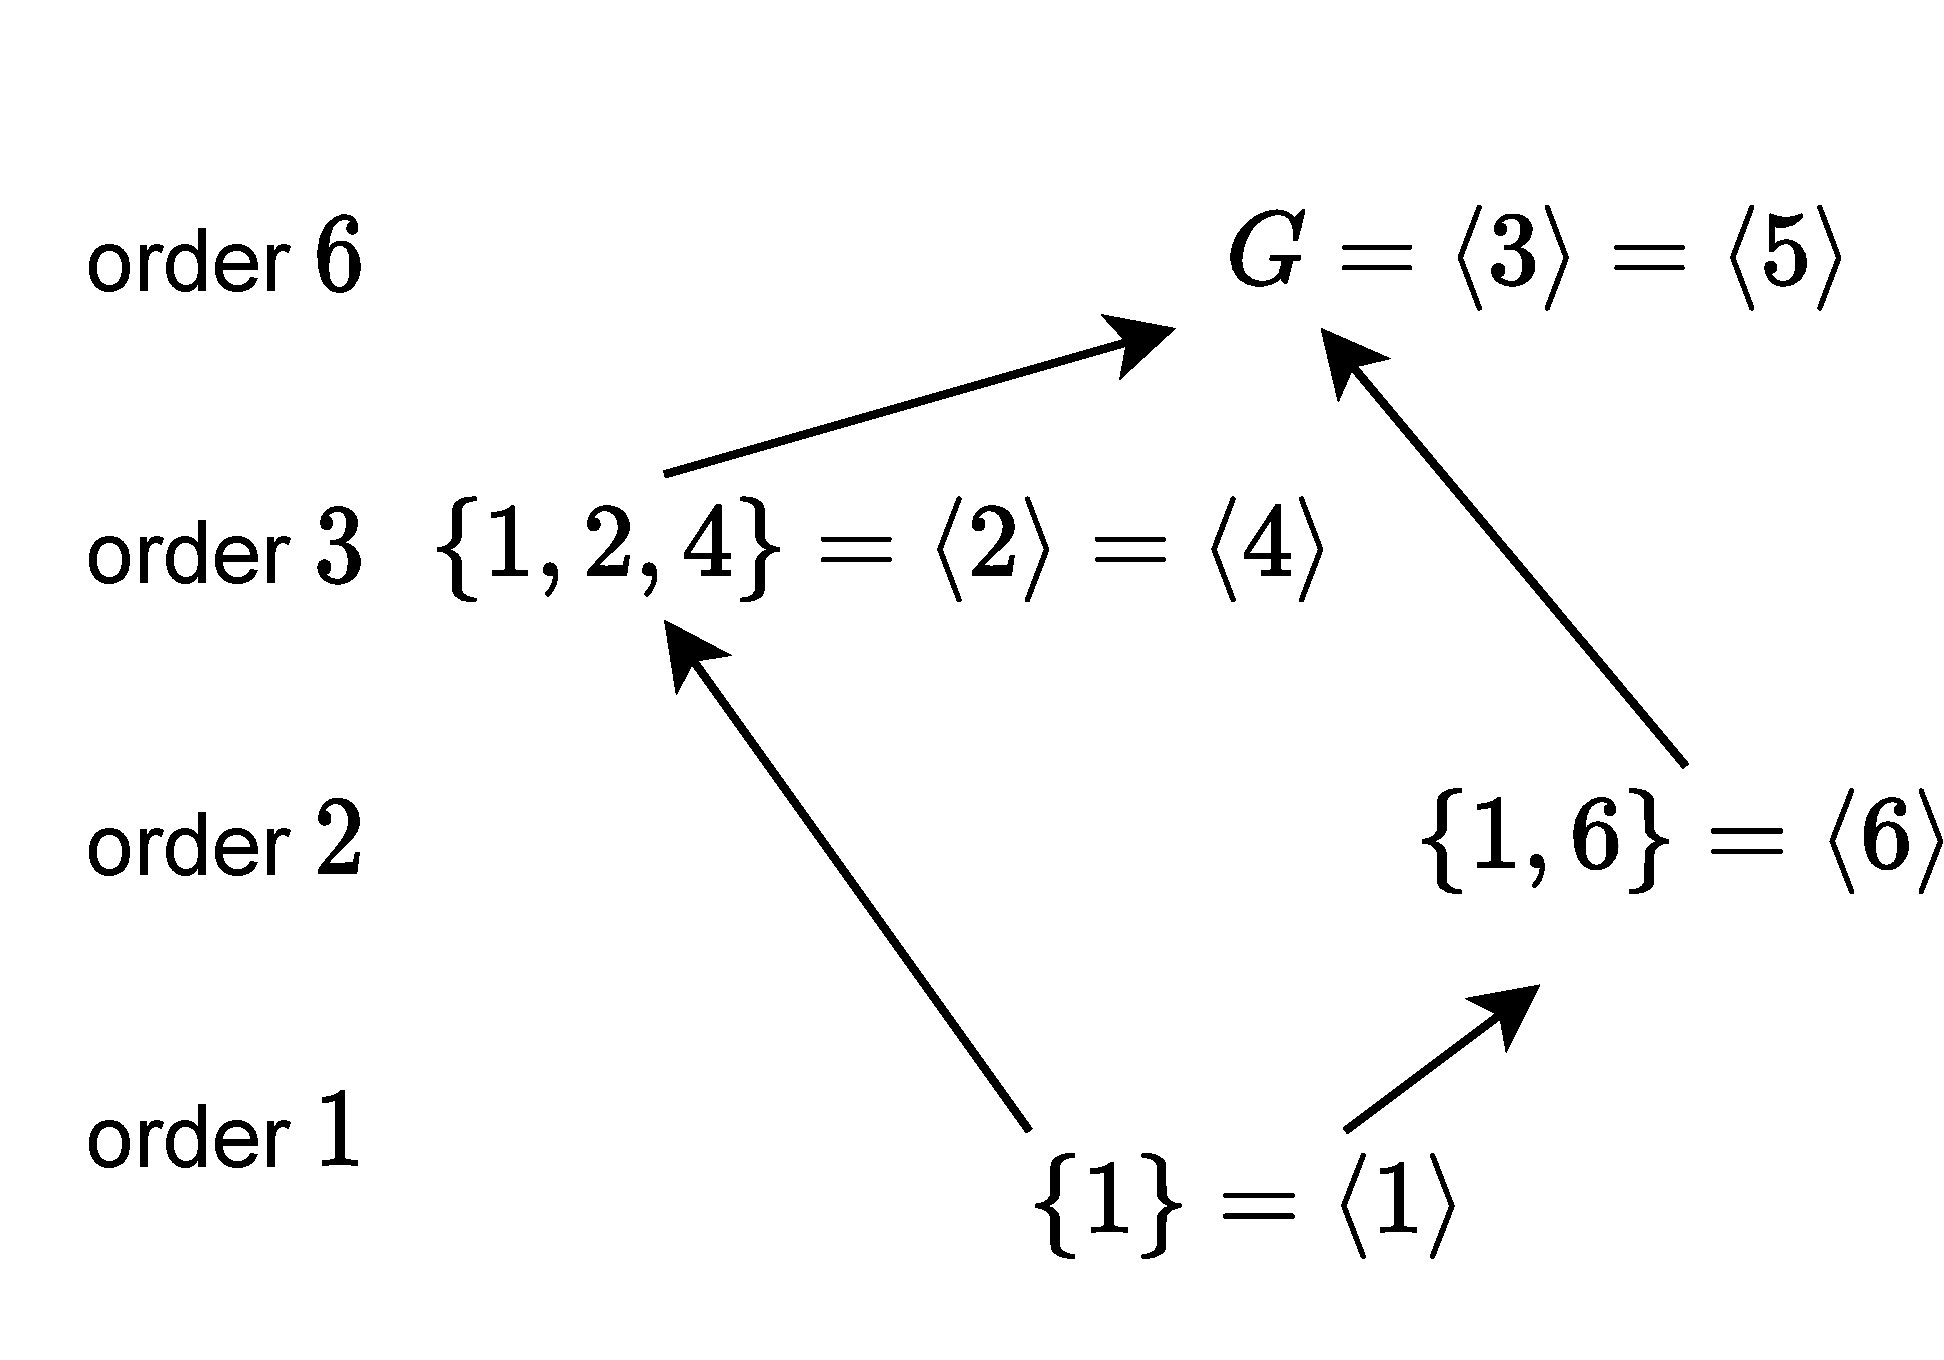
\includegraphics[width=0.5\textwidth]{Figures/Subgroup Lattice example.pdf}
    \caption{Subgroup Lattice for $G=\{1,2,3,4,5,6\}$ under multiplication $\mod 7$. Objects in this lattice are the subgroups of $G$, Arrows in this diagram correspond to the \textit{partial order} of set inclusion, where an arrow exists from $A\rightarrow B \iff A\subset B$}
    \label{fig:Subgroup_lattice}
\end{figure}
\newpage
\begin{proposition}[a.k.a Prop $\clubsuit$ (or \#27 from pg. 47 in Herstein)]
Every subgroup of a cyclic group is cyclic.\\
\textit{Proof:} Assume $G$ is cyclic with generator $a$, $a\in G$.
\begin{align}
    G=\langle a\rangle= \{a^n|n\in \Z\} \nonumber
\end{align}
\begin{enumerate}
    \item The trivial subgroup, $e$, is cyclic.
    \item Suppose that $H<G$ is a non-trivial subgroup of $G$  ($H\neq \{e\}$), then $\exists x\in H, x\neq e$ and since $H<G \implies x^{-1}\in H$.
    \begin{align}
        x\in G \implies \exists \ k \in \Z \ni x&=a^k \ \ \text{ and so,} \nonumber \\
        x^{-1}&=(a^k)^{-1}=a^{-k} \nonumber
    \end{align}
    Since either $k$ or $-k$ is positive, $H$ contains at least one positive power of $a$.\\
    Consider the smallest positive integer $n$ such that $a^n\in H$.\\
    \textit{Claim:} $H=\langle a^n \rangle $.\\
    \textit{Proof:} We must show $H\subset \langle a^n \rangle$ and $ \langle a^n \rangle \subset H$ we begin with the latter of the containments.\\
    $\langle a^n \rangle \subset H:$ Since $a^n\in H$, and $H$ is closed and contains inverses of all its elements, $(a^n)^j\in H \ \forall \ j\in \Z$. $\therefore \langle a^n \rangle \subset H$.\steezybreak\\
    $ H\subset\langle a^n \rangle :$ Take $h\in H$. $h\in G \implies \exists m\in\Z \ni h=a^m$. Next, we will use the euclidean algorithm to "divide" (we use quotes because $r$ may not equal $0$, "divide" in the grade school sense) $m$ by $n$.
    \begin{align}
        &\text{Eucl. Alg. } \implies \ \exists \ q,r\in \Z \ni \ m=qn+r, \ \ \text{ where } 0\leq r < n \nonumber \\
        &\text{then  }h=a^m=a^{qn+r}=(a^n)^q a^r \ \ \ \ (\text{Idea: show }r=0)\nonumber
    \end{align}
    Note that $(a^n)^q \in H \text{ by closure since } a^n \in H \implies [(a^n)^q]^{-1}\in H$. Therefore we can see $a^r$ is a member by closure
    \begin{align}
        a^r=[(a^n)^q]^{-1}\cdot h, \ \ \therefore a^r\in H \nonumber
    \end{align}
    Now we note again that $0\leq r < n$, $n$ is the \textit{smallest} positive integer $\ni a^n\in H \implies r$ can't be positive otherwise the definition of $n$ is violated. $\therefore r=0$.
    \begin{align}
        &\therefore \ h= (a^n)^q\cdot a^0 = a^{nq}\in \langle a^n \rangle \nonumber \\
        &\therefore H\subset \langle a^n \rangle \nonumber
    \end{align}
\end{enumerate}
\indent $\ \ \ \ \ \ \ \ \ \ \therefore H=\langle a^n \rangle.  \ \ \ \ \ \ \ \ \blacksquare$
\end{proposition}

\begin{definition}[Congruence mod $H$]
$H<G$, $G$ is a group. For $a,b\in G$, a is congruent to $b\mod H$, denoted
\begin{align}
    a\equiv b \mod H \iff ab^{-1}\in H \nonumber
    \end{align}
\end{definition}

\begin{example}
The definition above is the generalization of "congruence mod $n$" in $\Z$. Recall $n\Z \subset \Z$.
\begin{align}
    a\equiv b\mod (n\Z) &\iff ab^{-1}\in n\Z \ \ \ \ \ \text{(abstract notation)}\nonumber \\
     &\iff a-b \in n\Z \ \ \ \ \ \text{(specific to example)}\nonumber \\
     &\iff a-b \text{ is and integer multiple of }n \nonumber \\
     &\iff n|a-b \nonumber \\
     &\iff a\equiv b\mod n \nonumber 
\end{align}
\end{example}
\begin{lemma}
Congruence $\mod H$ is an equivalence relation on $G$.\\
\textit{Proof:}\\
\begin{enumerate}
    \item \textit{Reflexivity:} $\forall a \in G, aa^{-1}=e\in H$ so $a\equiv a \mod H$.
    \item \textit{Symmetry:} if $a\equiv b \mod H \implies ab^{-1}\in H$, $H$ is a subgroup so it must contain $(ab^{-1})^{-1}$.
    \begin{align}
        (ab^{-1})^{-1}=(b^{-1})^{-1}a^{-1}=ba^{-1} \ \ \ \text{ Lemma 2.3.1 } \nonumber \\
        \therefore ba^{-1}\in H \nonumber
    \end{align}
    so symmetry holds.
    \item \textit{Transitivity:} Assume $a\equiv b \mod H$ and $b\equiv c \mod H$ for $a,b,c \in G$. Then,
    \begin{align}
        ab^{-1}\in H \nonumber \\
        bc^{-1}\in H \nonumber \\
        ab^{-1}\cdot bc^{-1}\in H \ \ \ \ \text{ by closure}\nonumber \\
        \implies aec^{-1}\in H \implies ac^{-1}\in H \nonumber
    \end{align}
    therefore $a\equiv c \mod H$, $\equiv \mod H$ is transitive. $\ \ \ \ \blacksquare$
\end{enumerate}
\textit{Notation:} As in the special case where $G=\Z$, $[a]$ denotes the equivalence class (congruence class) of $a$:
\begin{align}
    [a]&=\{x\in G \ | \ a\equiv x\mod H\} \nonumber \\
    &=\{x\in G \ | \ a x^{-1} \in H\} \nonumber
\end{align}
\end{lemma}
\begin{definition}[Cosets]
$H<G$, $a\in G$. Define $Ha=\{ha|h\in H\}$, $Ha$ is called a right coset of $H$ in $G$.\\
(similarly, $aH=\{ah|h\in H\}$ is a left coset.)
\end{definition}
\begin{lemma}
$\forall a\in G, Ha=[a]$.\\
\textit{Proof:}\steezybreak\\
\textit{$Ha\subset [a]$:} \\ 
Take $ha\in Ha$. We need to get $ha\in [a]$.
\begin{align}
    ha\in[a] &\iff a\equiv ha \mod H \nonumber\\
    &\iff a (ha)^{-1} \in H \nonumber
\end{align}
Well let's check what $a(ha)^{-1}$ is.
\begin{align}
    a(ha)^{-1}&= a(a^{-1}h^{-1}) \ \ \ \ \text{By Lemma 2.3.1} \nonumber  \\
              &= (aa^{-1})h^{-1} \nonumber \\
              &= eh^{-1} \nonumber \\
              &= h^{-1} \nonumber 
\end{align}
Since $h\in H$, $h^{-1}\in H$, therefore $ha\in [a]$, and so $H\subset [a]$.\steezybreak\\
\textit{$[a]\subset Ha$:} \\
Take $x\in [a]$. Then $a\equiv x \mod H$ so $ax^{-1}\in H$. $H<G$ so $(ax^{-1})^{-1}\in H \underset{L 2.3.1}{\implies} xa^{-1}\in H$. \\
So $x=x\cdot e=x(a^{-1}a)=(xa^{-1})a\in Ha$. Therefore $H\subset [a]$.\\
$\therefore Ha=[a]$. $\ \ \ \ \ \ \ \blacksquare$
\end{lemma}
\setcounter{dummy_lemma}{3}
\begin{corollary}
If $Ha$ and $Hb$ are right cosets of $H$ in $G$, then either $Ha=Hb$ or $Ha\cap Hb=\emptyset$.\\
\textit{Proof:} This fact follows directly from Lemma 2.4.4 (above) and Thm 1.1.1. Under any equivalence relation, classes are either identical or disjoint. $\blacksquare$
\end{corollary}
Having seen this corollary, we can draw a picture representing $G$ and the various cosets of $G$'s subgroup $H$ like in Figure \ref{fig:cosets_fig}.
\begin{figure}[h!]
    \centering
    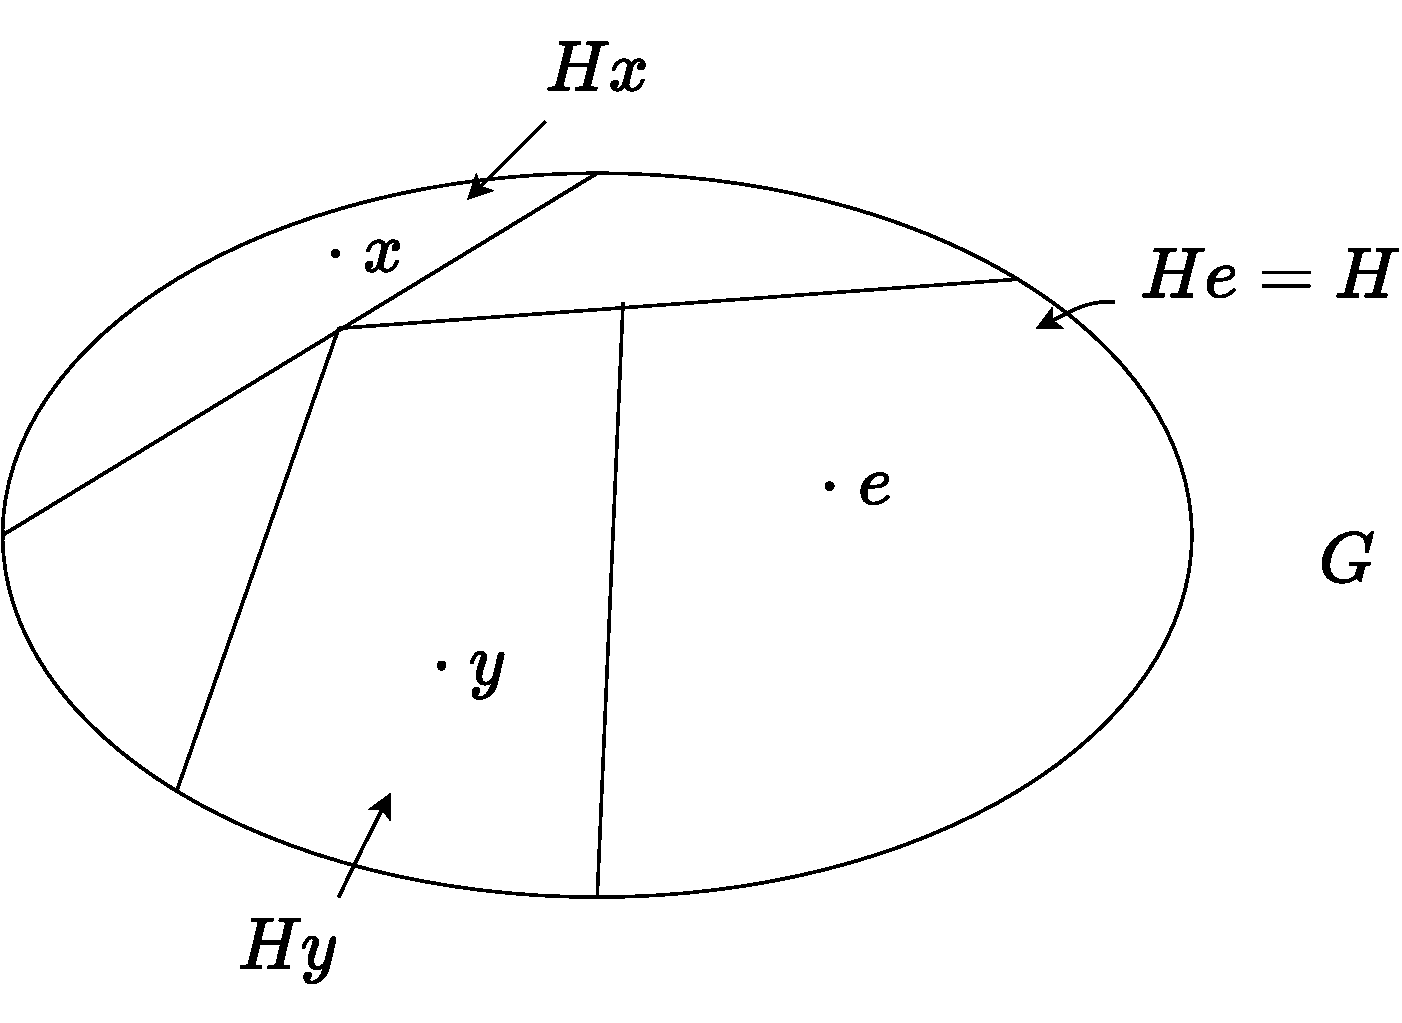
\includegraphics[width=0.6\textwidth]{Figures/Cosets_pic.pdf}
    \caption{Cosets of $H$ in $G$}
    \label{fig:cosets_fig}
\end{figure}
\begin{lemma}
If $Ha$ and $Hb$ are right cosets of $H$ in $G$, there is a bijection (1-1 correspondence) between them.\\
\textit{Proof:}\\
Define $\sigma: Ha\rightarrow Hb$ by
\begin{align}
    \sigma(ha)=hb \nonumber
\end{align}
\textit{$\sigma$ is surjective:} Take $y\in Hb$, then $\exists \ h\in H\ni y=hb$, so $\sigma(ha)=hb=y$. Since $ha$ serves as a preimage for $y$, $\sigma$ is surjective.\\
\textit{$\sigma$ is injective:} Take $x,y \in Ha $, $x\neq y$.
\begin{align}
    x,y &\in Ha \implies \exists \ \ h_1,\ h_2\in H\ni \ h_1a=x, \ \ h_2a=y \nonumber \\
    \sigma(x)&=\sigma(h_1 a)=h_1 b \nonumber \\
    \sigma(y)&=\sigma(h_2 a)=h_2 b \nonumber
\end{align}
Now, if $h_1b=h_2b$, then $b^{-1}\in G \implies h_1=h_2$ but this then implies that $h_1a=h_2a$, but this contradicts $x\neq y, \ \Rightarrow \Leftarrow$! So it must be true that $\sigma(x)\neq \sigma(y)$.\\
$\therefore \ \sigma$ injective. $\blacksquare$ 
\end{lemma}
\setcounter{dummy_lemma}{4}
\begin{corollary}
If $H$ is finite, then all the right cosets of $G$ have the same number of elements, namely $o(H)$.\\
\textit{Proof:} $H$ finite $\implies$ $Ha$ finite $\forall a \in G$, and the bijection from Lemma 2.4.5 guarantees uniform size. Since $H$ is one of the cosets ($He$) the size of each coset is the size of $H$. $\ \ \ \ \ \blacksquare$
\end{corollary} 

\subsection{Lagrange's Theorem (1770)} 
Joseph-Louis Lagrange was an Italian-born mathematician who was naturalized as a French citizen during adulthood. He lived from 1736 until 1813. Lagrange's work in number theory and math analysis had great influence on a young \'Evariste Galois (born 1811). Two of Lagrange's doctoral students include Joseph Fourier and Sim\'eon Poisson.
\setcounter{dummy}{0}
\begin{theorem}[Lagrange's Theorem] \hspace{0.1in}\steezybreak\\
If $G$ is a finite order group and $H<G$, then $o(H)|o(G)$.\steezybreak\\
\textit{Proof:} Suppose $H=\{h_1,...,h_r\}$ where $h_1=e$, so $o(H)=r$. \\
If $H=G$, then $o(G)=r$ so $o(H)|o(G)$.\\
Now let's consider $H\subset G$ with $H\neq G$. Then $\exists \ a\in G\ni a\not \in H$. So far we can find 2 disjoint cosets:
\begin{align}
    H=He&=\{h_1,...,h_r\}  \ \ \ \ \ &\text{note }h_1&=e\nonumber \\
    Ha&=\{h_1a,...,h_ra\} \ \ \ &\text{note }h_1a&=a\nonumber
\end{align}
If this accounts for all of the elements in $G$ then $o(G)=2o(H)$, so $o(H)|o(G)$. Otherwise, $\exists b \in G$, $b\not \in H\cup Ha$, we can use $b$ to build another coset:
\begin{align}
    Hb=\{h_1b,...,h_rb\}\nonumber
\end{align}
disjoint from the previous ones. We can continue in this way, producing cosets different from the previous ones, until $G$ is exhausted ($G$ finite). Eventually we will end up with $k$ (an integer) cosets each with $r$ elements. Then $o(G)=k o(H)$ since $k\in \Z$, $o(H)|o(G)$. $\blacksquare$
\end{theorem}
\begin{definition}[Index of a Subgroup]
for $H<G$, the \textit{index of} $H$ \textit{in} $G$, denoted:
\begin{align}
    i_G(H) &= \text{\# of right cosets of }H \text{ in } G \nonumber \\
    &= \frac{o(G)}{o(H)} \nonumber
\end{align}
is the number of distinct right cosets of $H$ in $G$ ("$k$" in the proof of Lagrange's Thm.)
\end{definition}
We will now present five important corollaries of Lagrange's theorem. Corollary 5 will be proven first as it is parallel to the other 4 corollaries (Cor 5. follows directly from Lagrange and does not require, nor suffice for, Cors 1.- 4.) and then we will prove a chain of corollaries as we have depicted in Figure \ref{fig:Lagrange_corrs}
\begin{figure}[ht!]
    \centering
    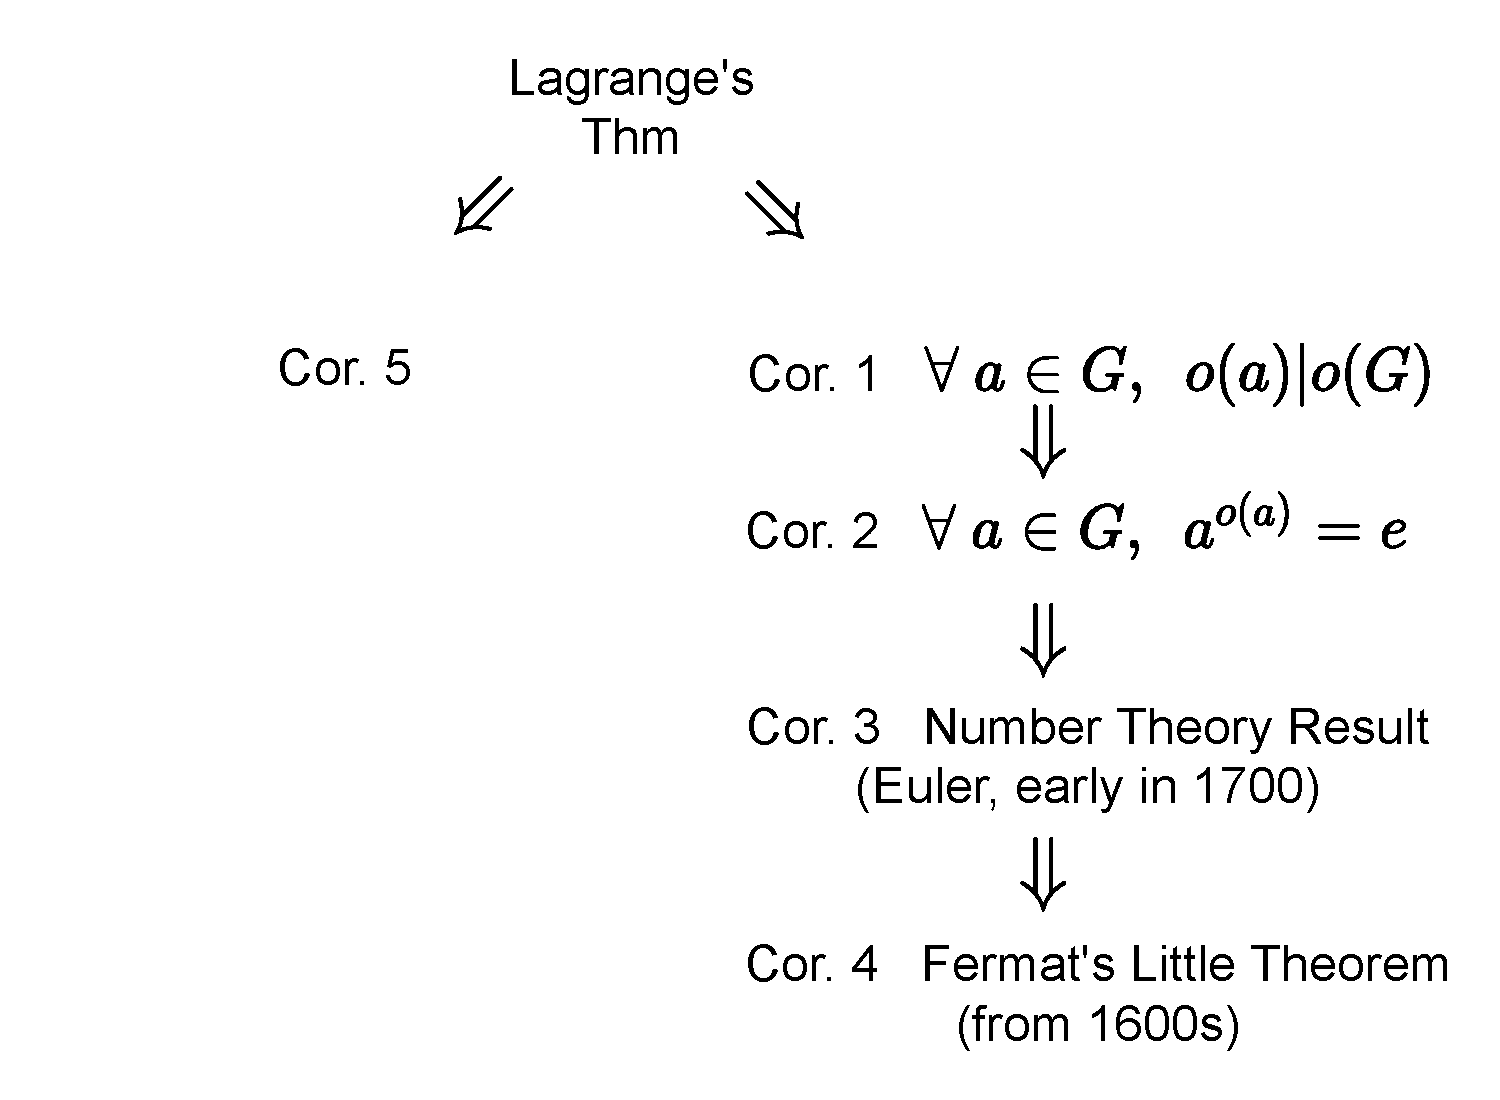
\includegraphics[width=0.6\textwidth]{Figures/Lagrange_corrollaries.pdf}
    \vspace{-0.1in}\caption{Five Corollaries of Lagrange's Theorem}
    \label{fig:Lagrange_corrs}
\end{figure}
\newpage
\setcounter{dummy_lemma}{0}
\begin{corollary}[Lagrange Cor. 5] 
If $G$ is finite, and $o(G)=p$ is prime, then $G$ is cyclic and has no non-trivial subgroups. \\
\textit{Proof:} Say $H<G$, Lagrange says $o(H)|o(G)$, so $o(H)$ can be $1$ or $p$.
\begin{align}
    \text{if }o(H)&=1, \text{ then } H=\{e\}, \text{ trivial.} \ \nonumber\\
    \text{if }o(H)&=p, \text{ then } H=G, \text{ trivial.} \ \nonumber
\end{align}
$o(G)$ prime means $\exists \ a\in G\ni a\neq e$. Consider the subgroup generated by $a$.
\begin{align}
    \langle a \rangle= \{a^n|n\in \Z\}\nonumber
\end{align}
Now, $\langle a \rangle < G \ \implies \langle a \rangle= G$ or $\langle a \rangle =\{e \}$, however since $a$ was non-trivial the second of these possibilities cannot occur.\\
$\therefore \langle a \rangle = G$. $\blacksquare$
\end{corollary}
One should note that when $o(G)$ prime, the proof provided above implies that ANY non-identity $a\in G$ can generate $G$ (In the proof we say we know AT LEAST one must exist because $p$ prime implies $p>1$ but this generating property holds for any $a\in G\ni$  $a\neq e$.)

\setcounter{dummy_lemma}{0}
\begin{corollary}[Lagrange Cor. 1]
$G$ a finite group, then $a\in G \implies o(a)|o(G)$.\\
\textit{Proof:} Say $o(a)=m$ and consider $H=\langle a \rangle =\{e,a^1,a^2,...,a^{m-1}\}$, note $e=a^0=a^m$.\steezybreak\\
Are these all different? Suppose $H$ has a repeat:
\begin{align}
    a^i=a^j \ &\text{ for some } 0\leq i < j \leq m-1 \nonumber \\
    &\implies a^ia^{-i}=a^{j-i} \nonumber \\
    &\iff e=a^{j-i}, \ \text{and } 0<j-i\leq m-1-i < m \nonumber
\end{align}
This is a contradiction of the definition of $o(a)$ (\textit{smallest} positive integer, $m$, power of $a$ such that $a^m=e$) $\Rightarrow \Leftarrow$. So $H$ has $m$ elements ($o(H)=m$).\\
Lagrange $\implies$ $o(H)|o(G) \ \implies o(a)|o(G). \ \  \blacksquare$
\end{corollary}

\setcounter{dummy_lemma}{0}
\begin{corollary}[Lagrange Cor. 2]
$G$ a finite group, with $a\in G$, then it must be true that $a^{o(G)}=e$.\\
\textit{Proof:} Cor 1. $\implies$ $o(a)|o(G) \ \implies \exists \ n\in \Z \ni o(G)=n(o(a))$, now calculate $a^{o(G)}$...
\begin{align}
    a^{o(G)}=a^{n(o(a))}=[a^{o(a)}]^n=[e]^n=e^n=e. \ \ \blacksquare \nonumber
\end{align}
\end{corollary}
Before we present and prove Corollary 3, we need one more definition and we will look at an example of it and a family of groups closely related to this newly defined function.
\begin{definition}[Euler Totient Function (Euler $\phi$-function)]
The Euler $\phi$-function (a.k.a The Euler Totient Function):\\
\begin{align}
    &\phi : \Z^+\rightarrow \Z^+ \ \ \text{ is a mapping from positive integers to positive integers defined as follows:}\nonumber \\
    &\phi(1)=1 \nonumber \\
    &\phi(n)=\text{the number of positive integers }<n\text{ and relatively prime to }n \nonumber
\end{align}
\end{definition}

\begin{example}
What is $\phi(10)$?, to find out, we look at the numbers less than 10 and greater than 0, and throw out any numbers who share factors with 10.
\begin{align}
1,2,3,4,5,6,7,8,9 \nonumber \\
1,\not 2, 3,\not 4, \not 5, \not 6,7,\not 8, 9 \nonumber \\
\underset{1}{1},\not 2, \underset{2}{3},\not 4, \not 5, \not 6,\underset{3}{7},\not 8, \underset{4}{9} \nonumber \\
\therefore \phi(10)=4. \nonumber \\
\text{Also note, for any prime number }p, \ \ \phi(p)=p-1 \nonumber
\end{align}
\end{example}

\begin{example}
For $n\in \Z^+$, define $G_n=\{m\in \Z^+ | m<n \text{ and } GCD(m,n)=1\}$. $G_n$ is a group under multiplication mod $n$. This family of groups is referred to as \textit{"The multiplicative group of integers modulo $n$"}, e.g. 
\begin{align}
    G_{10}= \{1,3,7,9\} \ \text{ under mult. mod }10 \nonumber \\
    G_{7}= \{1,2,3,4,5,6\} \ \text{ under mult. mod }7 \nonumber 
\end{align}
For this family of groups, we have that $o(G_n)=\phi(n)$. Ok we've introduced enough to talk about Cor. 3.
\end{example}

\setcounter{dummy_lemma}{0}
\begin{corollary}[Lagrange Cor. 3 (Euler)]
If $n\in \Z^+$ and $a\in \Z$ with $GCD(a,n)=1$, then $a^{\phi(n)}\equiv 1 \mod n$. \steezybreak\\
\textit{Proof:} We will consider two cases $n=1$ and $n>1$ and show the fact is true under either scenario. \steezybreak\\
If $n=1$, then $\phi(1)=1$ and $\forall a \in \Z$, $GCD(a,1)=1$, also $a\equiv 1 \mod 1$ because $1|(a-1)$.\steezybreak\\
If $n>1$, take any $a\in \Z \ni GCD(a,n)=1$. Euclidean Alg. $\implies \exists \ q,r \in \Z \ni a=qn+r$. Where $0\leq r < n$.\steezybreak\\
\textit{Claim:} $r\in G_n$ (must show $r\neq 0$, $GCD(r,n)=1$). \\
\textit{Proof of Claim: }If $r=0$, then $a=qn$, so $n|a$, and $GCD(a,n)=n\neq 1$ $\Rightarrow\Leftarrow$. So $r$ is a positive integer $<  n$. \steezybreak\\
Say $GCD(r,n)=d$, then $d|r$ and $d|n$, and by observation \#4, $d|a$, a linear combination of $r$ and $n$. Since $d|a$ and $d|n$, $d|GCD(a,n)$. But $GCD(a,n)=1$ by assumption so by observation \#1 about divisions, $\implies d= \pm 1 \implies d= 1$, so $r$ and $n$ are relatively prime $\blacksquare$ (end of proof of supporting claim, Cor. 3 proof continues).\steezybreak\\
Apply Cor \# 2: $G_n$ finite group, $r\in G_n$. $o(G_n)=\phi(n)$, so $r^{\phi(n)}=1$ ($1$ is $e$ in $G_n$).\\
In the language of $\Z$
\begin{align}
    &r^{\phi(n)}\equiv 1 \mod n\nonumber \\
    \text{Now, } a=qn+r &\implies a\equiv r \mod n \nonumber \\
    &\implies a^{\phi(n)} \equiv r^{\phi(n)}\mod n \nonumber \\
    &\therefore \text{ by transitivity of }\equiv \mod n, \ a^{\phi(n)}\equiv 1 \mod n \ \ \ \blacksquare \nonumber 
\end{align}
\end{corollary}

\begin{example}
Reduce $2^{523}\mod 11$.
\begin{align}
    a&=2 \nonumber \\
    n&=11 \ \ \textit{prime} \nonumber \\
    \phi(n)&= 10 \nonumber \\
    \text{Euler Cor. }&\implies 2^{10}\equiv 1 \mod 11 \nonumber \\
    &\implies (2^{10})^{52}\equiv 1^{52}\mod 11 \nonumber \\
    &\implies 2^{520}\equiv 1 \mod 11 \nonumber \\
    2^3&\equiv 2^3\mod 11 \ \ \ (\equiv \mod n \text{ is reflexive})\nonumber \\
    2^{523}&\equiv 1\cdot 2^{3}\mod 11\nonumber \\
    \therefore 2^{523}&\equiv 8 \mod 11 . \nonumber
\end{align}
\end{example}
%\newpage
\setcounter{dummy_lemma}{0}
\begin{corollary}[Lagrange Cor. 4 (Fermat's "Little Theorem")]
$p$ prime and $a\in \Z$, then $a^p\equiv a \mod p$. \\
\textit{Proof:} $p$ prime $\implies \phi(p)=p-1$. Take any $a\in \Z$, then $GCD(a,p)=1$ or $p$. \\
If $GCD(a,p)=1$, then $a$ is relatively prime to $p$
\begin{align}
    \implies &a^{p-1}\equiv 1\mod p \ \ \text{ Cor. 3}\nonumber \\
    &a\equiv a \mod p \ \ \text{ reflexivity } \nonumber \\
    \text{Lemma 1.3.3 (3) }\implies &a^p\equiv a\mod p \nonumber 
\end{align}
If $GCD(a,p)=p$, then $p|a$, so 
\begin{align}
    &a\equiv 0 \mod p \ \ \ (\text{ or } 0\equiv a \mod p \text{ by symmetry})\nonumber \\
    &\implies a^p\equiv \underset{=0}{0^p}\mod p \nonumber \\
    &\text{By transitivity, }a^p\equiv a \mod p. \ \ \ \blacksquare \nonumber
\end{align}
\end{corollary}

\begin{example}
\textit{Problem:} find a polynomial of degree $3$ with integer coefficients and leading coefficient $1$ that sends every integer to a multiple of 3.
\begin{align}
    f(x)&=x^3+bx^2+cx+d, \ \ \ \ b,c,d \ \in \Z \nonumber \\
    \forall a \in \Z \text{ we want } &f(a)\in 3\Z \nonumber \\
    f(a)\in 3\Z \iff f(a)&\equiv 0 \mod 3. \nonumber \\
    \text{Fermat } \implies a^3&\equiv a \mod 3  \nonumber \\
    \text{ (Add) }\ \ \ \ \ -a&\equiv -a\mod 3 \ \ \ \text{(reflexivity)}  \nonumber \\
    a^3-a&\equiv 0 \mod 3 \nonumber \\
    \therefore \text{ take } f(x)= x^3 - x. \nonumber 
\end{align}
\end{example}
\steezybreak
\begin{tcolorbox}
\begin{center}
    $\star\star\star$ \textbf{Read up to this point to Complete Homework 4} $\star\star\star$
\end{center}
\end{tcolorbox}
\newpage
\section{A Counting Principle}
The next question that we will explore is the following: Given $H,K < G$, can we make a subgroup from $H$ and $K$ which contains both...\steezybreak\\

\noindent What about $H\cup K$? \\ 
Recall example $G_7=\{1,2,3,4,5,6\}$ under multiply $\mod 7$. We found 
\begin{align}
    H&=\langle 2 \rangle = \{2,4,1\} \nonumber \\
    K&=\langle 6 \rangle = \{1,6 \} \nonumber \\
    H\cup K &= \{1,2,4,6\} \not < G, \text{ because } 4 \not | \ 6 (\text{ Lagrange Thm Violated}) \nonumber
\end{align}

\begin{definition}[Set Product]
Given $H,K < G$. The \textit{Set Product} of $H$ and $K$, denoted $HK$, is defined as follows:\\
\begin{align}
HK = \{hk \ | \ h\in H,k\in K\} \nonumber
\end{align}
\end{definition}

\begin{lemma}
$H,K < G$, then $HK < G$ iff $HK=KH$. \steezybreak\\
\textit{Proof:} \\
$\Leftarrow :$ \\
Assume $HK=KH$, we will use Lemma 2.4.1, which applies since $HK\neq \emptyset; \ \ e\cdot e = e\in HK$.
\begin{enumerate}
    \item Show $HK$ is closed. Take $x,y\in HK$,
    \begin{align}
        x\in HK &\implies \exists \ h \in H, k\in K \ni x=hk \nonumber \\
        y\in HK &\implies \exists \ h' \in H, k'\in K \ni y=h'k' \nonumber \\
        xy&=(hk)(h'k')=h(kh')k' \nonumber \\
        \text{Now, } kh'\in KH&=HK\implies \ \exists \ \hat{h}\in H, \hat{k}\in K \ni kh'=\hat{h}\hat{k} \nonumber \\
        \text{So } xy&=h(\hat{h}\hat{k})k'= \underset{\in H}{(h\hat{h})}\underset{\in K}{(\hat{k} k')} \in HK \nonumber
    \end{align}
    \item Inverses. Take $x$ as above ($x \in HK$ so $\exists h \in H, k\in K \ni x=hk$) \\
    \begin{align}
        x^{-1}=(hk)^{-1}=k^{-1}h^{-1}\in KH = HK \nonumber
    \end{align}
\end{enumerate}
$\Rightarrow :$ \\
Assume $HK<G$ show that $HK=KH$.
\begin{align}
    \text{Take }x &\in KH \text{ then }x^{-1}\in HK \nonumber\\
    &\therefore \ \exists \ \bar{h} \in H, \bar{k}\in K \ni x^{-1}=\bar{h}\bar{k} \nonumber \\
    &x=(x^{-1})^{-1}=(\bar{h}\bar{k})^{-1}=\bar{k}^{-1}\bar{h}^{-1}\in KH \nonumber \\
    &\therefore HK \subset KH. \nonumber
\end{align}
Now, let $x\in KH$ (we will show the other containment), $x\in KH$ implies the existence of two elements
\begin{align}
    &\exists \ k \in K, h \in H \ni x= kh \nonumber\\
    &x^{-1}= (kh)^{-1}=h^{-1}k^{-1}\in HK \nonumber \\
    &\therefore (x^{-1})^{-1} \in HK \ \text{( remember $HK$ is assumed a subgroup!) } \nonumber \\
    &\therefore x \in HK \nonumber \\
    &\therefore KH\subset HK, \text{ so } HK=KH. \ \ \ \ \ \ \ \ \ \blacksquare \nonumber
\end{align}
\end{lemma}
\setcounter{dummy_lemma}{0}
\begin{corollary}
If $H,K < G$ and $G$ is abelian, then $HK<G$.\\
\textit{Proof:}
$G$ abelian means $hk=kh$ $\forall \ h\in H, \ k\in K$. So we get $HK=KH$ for free and L 2.5.1 applies. $\blacksquare$
\end{corollary}

\begin{theorem}
$H, K$ finite subgroups of $G$. Then $o(HK)= \frac{o(H)o(K)}{o(H\cap K)}$ \steezybreak\\
(Note, this is true whether or not $HK$ is a subgroup! In the proof you will see we only rely on $H$ and $K$ \textit{themselves} being subgroups, we don't require that $HK$ is a subgroup) \steezybreak\\
\textit{Proof:} If we list elements of $HK$ including possible duplicates, there would be $o(H)\cdot o(K)$ products in the list. Take $g$ in the list, then 
\begin{align}
    \exists \ h\in H \text{ and } k\in K \ni g=hk.\nonumber
\end{align}
How many times does $g$ appear in the list? What other ways are there to write $g$ as $(\text{elt. of }H)(\text{elt. of} K)$... Suppose there were another way to write $g$ as $(\text{elt. of }H)(\text{elt. of} K)$:
\begin{align}
    g&=hk=\tilde{h}\tilde{k} \nonumber \\
    &\implies \tilde{h}=hk\tilde{k}^{-1}  \text{ and } \tilde{k}=\tilde{h}^{-1}hk \nonumber
\end{align}
Let's call $k\tilde{k}^{-1} =x \in K$. \steezybreak\\
\textit{Claim:} $\tilde{h}^{-1}h$ is $x^{-1}$.\\
\textit{Proof of Claim:}
\begin{align}
    x^{-1}&=(k\tilde{k}^{-1})^{-1}= \tilde{k}k^{-1}=\tilde{h}^{-1}hkk^{-1}=\tilde{h}^{-1}h\cdot e=\tilde{h}^{-1}h. \nonumber
\end{align}\steezybreak\\
$\therefore \ x^{-1} \in H < G \implies x \in H, \text{ thus } x\in H\cap K $ \\
So the only way to write $g$ differently than $hk$ is to write it $(h \star)(\star^{-1}k)$ where $\star \in H \cap K$ and $\star \neq e$. \\
Now, we note that for $x,y \in H\cap K$ if $x\neq y$ then $hx\neq hy$ by left cancellation. \\
Conclusion: Running through distinct elements of $H\cap K$ generates all of the ways $g$ can be expressed as (elt H)(elt K) so $g$ appears in the list $o(H\cap K)$ times. 
\begin{align}
    \underset{\text{No. distinct elements in $HK$}}{o(HK)}\cdot \underset{\text{No. times each appears}}{o(H\cap K)}= \underset{\text{No. elts in original list (including duplicates)}}{o(H)\cdot o(K)} \nonumber
\end{align}
Hence,
\begin{align}
    o(HK)=\frac{o(H)\cdot o(K)}{o(H\cap K)}. \ \ \ \ \ \ \ \ \blacksquare \nonumber
\end{align}
\end{theorem}
\newpage
\begin{corollary}
$G$ group with $o(G)=pq$, $p,q$ primes, $p>q$, then $G$ has no more than one subgroup of order $p$. \steezybreak\\
\textit{Proof:} Suppose $H,K<G$ have the same order (Aim: show $H=K$)
\begin{align}
    o(H)&=o(K)=P \ \ \ H,K \subset G \nonumber \\
    o(G)&\geq o(HK) = \frac{o(H)\cdot o(K)}{o(H\cap K)}= \frac{p\cdot p}{o(H\cap K)} > \frac{p\cdot q}{o(H\cap K)} = \frac{o(G)}{o(H\cap K)} \nonumber \\
    &\implies o(H\cap K)>1 \ \ \text{so }H\cap K\text{ is a non-trivial subgroup.} \nonumber
\end{align}
But $H\cap K < H \implies o(H\cap K)|o(H)$. Now, noting that $o(H)=p$ a prime, and since $o(H\cap K)\neq 1$ we are left to conclude that $o(H\cap K)=p$. This (the fact that $H\cap K$ has the same number of elements as $H$ and $K$), together with the following two obvious containments $H\cap K \subset H$ and $H\cap K \subset K$, implies that $H=H\cap K = K$.    \ \ \ \ \ $\blacksquare$
\end{corollary}

\steezybreak
\begin{tcolorbox}
\begin{center}
    $\star\star\star$ \textbf{\textit{~This Corr. marks the end of Test 1 Material for MTH 421 Course~}} $\star\star\star$ \\
    Do the Take Home Exam first, and then the In-Class Portion!
\end{center}
\end{tcolorbox}
\steezybreak
\section{Normal Subgroups and Quotient Groups}
In the proof of Lagrange's theorem, the reader probably recalls that we used this equivalence relation:
\begin{align}
    a\equiv b \mod H \iff ab^{-1}\in H \nonumber
\end{align}
under which $[x]\underset{L \ 2.4.4}{=}Hx$. \steezybreak\\
Let us now consider a slightly different relation:
\begin{align}
    a\equiv b \mod H \iff a^{-1}b\in H \nonumber
\end{align}
under this new relation, 
\begin{align}
    [x]=xH= \{xh|h\in H\} \nonumber
\end{align}
The classes are left cosets of $H<G$.\steezybreak\\
\textit{Question:} is the list of left cosets always the same as the list of right cosets? \steezybreak\\
Given $H<G$, is the list of right cosets of $H$ in $G$ the same as the list of left cosets of $H$ in $G$? Let's look at an example for some guidance.
\begin{example}
Consider again the group $S_3$.
\begin{align}
    G=\{I,\sigma,\tau,\sigma\tau,\tau\sigma,
    \sigma\tau\sigma \} \nonumber \\
    \sigma^2=I, \ \ \tau^2=I, \ \ \tau \sigma \tau = \sigma \tau \sigma. \nonumber
\end{align}
Let $H=\langle \sigma \rangle = \{I,\sigma \}$, now let's list the right cosets of $H$ in $S_3$:
\begin{align}
    i_{S_3}(H)&= \frac{o(S_3)}{o(H)}= \frac{6}{2}=3 \ \ \text{ So we expect 3 cosets each w/ 2 elts.} \nonumber \\ \nonumber \\
    HI &= H = \{\sigma, I\} \nonumber \\
    H\tau  &= \{\sigma\tau, \tau\} \nonumber \\
    H\tau\sigma  &= \{\sigma\tau\sigma, \tau\sigma\}=H\sigma\tau\sigma \nonumber \\
    H\sigma\tau  &= \{\sigma\tau, \tau\} = H\tau \nonumber 
\end{align}
So there were three unique ones as expected. Let's have a look at the left cosets:
\begin{align}
    IH  &= H= \{\sigma, I\}  \nonumber \\
    \tau H  &= \{\tau\sigma, \tau \}  \nonumber \\
    \sigma\tau H  &= \{\sigma\tau\sigma, \sigma\tau \}  \nonumber \\
    \tau\sigma H  &= \{\tau, \tau\sigma \} =\tau H \nonumber \\
    \sigma\tau\sigma H  &= \{\sigma\tau, \sigma\tau\sigma \} =\sigma\tau H \nonumber 
\end{align}
this example shows the answer is: not always.
\end{example}
\begin{definition}[Normal Subgroup]
A subgroup $N$ of $G$ is \textit{normal} in $G$ denoted $N \triangleleft G$ if $\forall g \in G$ and $\forall n \in N$ it is true that:
\begin{align}
gng^{-1}\in N \nonumber
\end{align}
(Taking the product $gng^{-1}$ is called "conjugating $n$ by $g$"; $gng^{-1}$ is the conjugate).\\
Alternately the definition can be written:
\begin{align}
    N \triangleleft G \iff gNg^{-1}\subset N \ \ \forall g \in G. \nonumber
\end{align}
\end{definition}


\begin{lemma}
Suppose $N<G$, then $N\triangleleft G \ \iff gNg^{-1} = N \ \forall \ g \in G$.\\
\textit{Proof:}\\
$\Leftarrow$: $gNg^{-1}= N \ \ \forall g \in G$ gives $gNg^{-1}\subset N \ \forall g \in G$ immediately so $N\triangleleft G$ by the equivalent definition. \\
$\Rightarrow$: Assume $N\triangleleft G$ we get $gNg^{-1}\subset N \ \forall g \in G$ by equivalent defn, all that remains is to show the other containment ($N \subset gNg^{-1}, \  \forall g \in G)$,\\
$\supseteq$: take $n\in N$, $g\in G$.
\begin{align}
    &n=e\cdot n\cdot e = g(\underset{\in N}{g^{-1}ng})g^{-1} \in gNg^{-1} \ \ \ \ \ \nonumber \\
    &\therefore N \subseteq gNg^{-1}. \ \ \ \ \ \ \ \ \ \ \ \ \ \ \ \ \ \ \blacksquare \nonumber 
\end{align}
(Remember $(elt)n(elt)^{-1}$, so $(g^{-1})n(g^{-1})^{-1} = g^{-1}ng$, this is how we can be sure that $g^{-1}ng \in N$ given the assumption, since $g^{-1}$ is just some other element in $G$ and the assumption says $(elt)n(elt)^{-1}$ in $N$ for ALL elements in $G$ !)
\end{lemma}

\begin{lemma}
Suppose $N< G$, then $N\triangleleft G \iff $ every left coset of $N$ in $G$ is a right coset of $N$ in $G$. \\
\textit{Proof:}\\
$\Rightarrow$: Assume $N\triangleleft G$.
\begin{align}
    \text{Lemma 2.6.1 }\implies gNg^{-1}= N \ \forall g \in G \nonumber \\
    \implies gN=Ng \ \ \forall g \in G. \nonumber
\end{align}
$\Leftarrow$: Take $g\in G$. $g$ sits in both $Ng$ and $gN$. Hypothesis says that $gN$ is some right coset, say $Na$.
\begin{align}
    g=ge\in g N = Na \nonumber \\
    \therefore g \in Na\cap Ng \nonumber
\end{align}
Right cosets are either disjoint or identical so we must have $Ng=Na$. So,
\begin{align}
    &gN=Ng \ \ \ \text{(Multiply each side on the right by $g^{-1}$)} \nonumber \\
    \implies &gNg^{-1}=N \nonumber \\
    &\therefore N \triangleleft G \text{ by L 2.6.1}. \ \ \ \blacksquare \nonumber 
\end{align}
\end{lemma}

\setcounter{dummy_lemma}{1}
\begin{corollary}[Corr. to L 2.6.2, a.k.a problem \# 2 from pg 53 of Herstein] 

If $H<G$ and $i_G(H)=2$, then $H\triangleleft G$. \\
\textit{Proof:}  $i_G(H)=2 \ \ \implies \ $ two right and two left cosets.\\
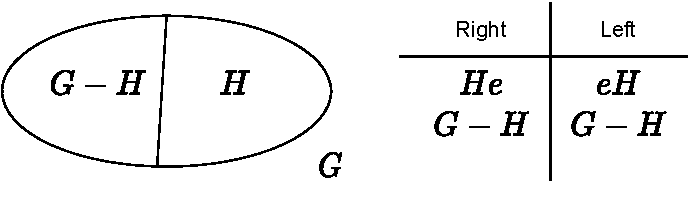
\includegraphics[width=0.65\textwidth]{Figures/as(1).pdf} \\($H=He$ is a right coset, and if there are only two right cosets then the remaining coset must be everything else in $G$, a similar argument can be made for $H's$ left cosets in $G$ )\\
So $H\triangleleft G$ by L 2.6.2. $\blacksquare$
\end{corollary}
Which subgroups have index 2? \ \ $i=2=\frac{o(G)}{o(H)}$ \steezybreak\\
\begin{center}
  $\implies$\ \ \ \ \boxed{o(H)=\frac{1}{2}o(G)}  
\end{center}\steezybreak
Note that according to the set product defn.
\begin{align}
    HK&=\{hk|h\in H, k\in K\} \nonumber 
    \end{align}
It is true for any subgroup $H<G$ that, 
\begin{align}
    HH&=H. \nonumber \\
    \textit{pf:} \ \ \ \ &\subseteq : \text{closure in } H \nonumber \\
    &\supseteq : h=\underset{\in H}{h}\cdot\underset{\in H}{ e} \in  HH \nonumber 
\end{align}
We use this fact in our proof of the lemma below.

\begin{lemma}
Suppose $N<G$. $N\triangleleft G \iff Na\cdot Nb = N{ab} \ \forall a,b \in G$ \steezybreak\\
\textit{Proof:} \steezybreak\\
$\Rightarrow :$  \ \ \ Assume $N\triangleleft G$\steezybreak\\
Take $a,b\in G$
\begin{align}
    NaNb=N(aN)b \underset{L \ 2.6.2}{=}N(Na)b=NNab = Nab .\nonumber
\end{align}
$\Leftarrow :$ \ \ \ Assume $Na\cdot Nb=Nab \ \forall a,b\in G.$\steezybreak\\
Take $a\in G$; we'll show $aN=Na$ (so $N\triangleleft G$ by L 2.6.2)\steezybreak\\
$\subseteq :$ ($aN\subseteq Na$ must be shown)
\begin{align}
    &NaNa^{-1}=Naa^{-1}=N \nonumber\\
    &\text{Right multiply by } a \nonumber\\
    &\implies NaN=Na \nonumber \\
    &aN=eaN\subseteq NaN=Na , \text{ so } aN\subseteq Na \nonumber
\end{align}
$\supseteq :$ ($Na\subseteq aN$ must be shown)\steezybreak\\
\begin{align}
    &Na^{-1}Na=Na^{-1}a=N \nonumber \\
    &\text{Right multiply by } a^{-1} \nonumber\\
    &\implies Na^{-1}N=Na^{-1}; a^{-1}N=ea^{-1}N\subseteq Na^{-1}N=Na^{-1} \nonumber \\
    &\text{So } a^{-1}N\subseteq Na^{-1} \nonumber \\
    &\implies a^{-1}Na\subset N \nonumber \\
    &\implies Na\subset aN \nonumber
\end{align}
$\therefore aN=Na$ and so $N\triangleleft G$ by L 2.6.2. $\blacksquare$
\end{lemma}
\subsubsection{Normal Subgroups Summary}
\begin{align}
    N\triangleleft G &\overset{defn.}{\iff} gng^{-1}\in N \ \ \forall \ n\in N \text{ and } \forall \ g \in G. \nonumber \\
    &\overset{}{\iff} gNg^{-1}\subset N \ \ \forall \ g \in G \nonumber \\
    &\overset{L2.6.1}{\iff} gNg^{-1} = N \ \ \forall \ g \in G \nonumber \\
    &\overset{L2.6.2}{\iff} gN = Ng \ \ \forall \ g \in G \nonumber \\
    &\overset{L2.6.3}{\iff} NaNb = Nab \ \ \forall \ a,b \in G \nonumber 
\end{align}
$N\triangleleft G$ means the set of cosets of $N$ in $G$ has a group structure.\steezybreak\\
$N\triangleleft G$ means:
\begin{enumerate}
    \item $N$ absorbs conjugates:
    \begin{align}
        gng^{-1}\in N \ \ \forall \ g \in G, \ \ \forall \ n \in N. \nonumber 
    \end{align}
    \item The left and right cosets of $N$ are equal
    \begin{align}
        gN=Ng \ \ \forall \ g \in G. \nonumber 
    \end{align}
    \item The cosets combine under binary operations:
    \begin{align}
        NaNb\overset{\star\star\star}{=}Nab \ \ \forall \ a,b \in G. \nonumber
    \end{align}
    \item With this ($\star\star\star$) operation, the cosets form a group (Thm 2.6.1)
\end{enumerate}
\begin{definition}[Quotient Group]
For group $G$ with normal subgroup $N\triangleleft G$, $G/N$ ($G \mod N$)
\begin{align}
    G/N\overset{def}{=}\{\text{(right) cosets of }N \text{ in } G\}\nonumber
\end{align}
\end{definition}
\newpage
\begin{theorem}[Quotient Groups] \hspace{0.01in}\\
if $N\triangleleft G$, then $G/N$ is a group under this operation:
\begin{align}
    Na \underset{\text{in }G/N}{\cdot} Nb = Na \underset{\text{in }G}{\cdot} b \nonumber
\end{align}
\textit{Proof:} We must show that $G/N$ under the defined operation follows the 4 group properties.
\begin{enumerate}[label=\roman*)]
    \item Closure:
    \begin{align}
        NaNb=Nab \nonumber
    \end{align}
    Since $Nab$ is a coset in $G/N$ we are done (closure is built into the defn of the operation)
    \item Associativity:
    \begin{align}
        [NaNb]Nc&=NabNc \nonumber\\
        &= N(ab)c \nonumber \\
        &= Na(bc)  \ \ \ \ (\text{since } G \text{ is assoc.})\nonumber \\
        &= Na(Nbc) \nonumber \\
        &= Na[NbNc] \nonumber
    \end{align}
    \item Identity:
    \begin{align}
        NaNe=Nae=Na\nonumber \\
        NeNa=Nea=Na\nonumber \\
        Ne=N \text{ is the } e \text{ in } G/N \nonumber
    \end{align}
    \item Inverses: $\text{Take }Na\in G/N.$
    \begin{align}
        a\in G &\implies a^{-1} \in G, \text{ so } Na^{-1}\in G/N \nonumber \\
        NaNa^{-1}&=Naa^{-1}=Ne=N \nonumber \\
        Na^{-1}Na&=Na^{-1}a=Ne=N \nonumber 
    \end{align}
    So $(Na)^{-1}=Na^{-1}$. \ \ \ \ \ $\blacksquare$
\end{enumerate}
    
$G/N$ is referred to as the \textit{quotient group} or \textit{factor group} of $G$ by $N$.
\end{theorem}
\begin{lemma}
if $N\triangleleft G$ finite, then
\begin{align}
    o(G/N)=\frac{o(G)}{o(N)}\nonumber
\end{align}
\textit{Proof:}
\begin{align}
    o(G/N)&= \# \text{ of (right) cosets of }N \text{ in }G \nonumber \\
    &= i_G(N)=\frac{o(G)}{o(N)}. \ \ \ \blacksquare \nonumber 
\end{align}
\end{lemma}

\begin{example}
$G=\Z$ under $+$
\begin{align}
    n\Z=\{\text{integer multiples of }n\}< \Z \nonumber
\end{align}
\textit{Claim:} $nZ\triangleleft \Z$, we'll show $n\Z$ absorbs conjugates ($\forall \ h\in H, \ \forall \ g\in G, ghg^{-1}\in H$).\\
Take $z\in \Z$ and $nm\in n\Z$.
\begin{align}
    \underset{g}{z}\ \ \ \ \underset{\cdot \text{ in } G}{+}\ \ \ \ \underset{h}{nm}\ \ \ \ +\ \ \ \ \underset{g^{-1}}{(-z)}=nm \in n\Z \ \ \ \ (\text{Remember that }\Z\text{ is abelian under }+) \nonumber
\end{align}
So $\Z/n\Z$ is a quotient group of $n\Z$ in $\Z$. What are it's elements?
\begin{align}
    G/N&= \{\text{(right) cosets of }N \text{ in }G\}\nonumber \\
    N\cdot 0 &= n\Z+0 = n\Z=[0] \text{ under }\equiv\mod n \nonumber \\
    N\cdot 1 &= n\Z+1 =[1] \text{ under }\equiv\mod n \nonumber \\
    N\cdot 2 &= n\Z+2 =[2] \nonumber\\
    \vdots \nonumber \\
    N\cdot (n-1)&= n\Z+n-1=[n-1] \nonumber \\
    N\cdot n&= n\Z+n=[0] \nonumber 
\end{align}
So $\Z/n\Z= \{[0],[1],[2],...,[n-1]\}$. So $\Z/n\Z$ and $\Z_n$ are the same group (rename the elements to get $\Z_n$).
\end{example}

\begin{example}
Passing from $G\rightarrow G/N$ lets you study properties of $G$ in a smaller group. For instance, oddness or evenness in $\Z$, use $\Z/2\Z$.\steezybreak\\
$\Z/2\Z=\{[0],[1]\}=\{2\Z+0,2\Z+1\}$ or $Z_2=\{0,1\}$ under addition $\equiv\mod 2$

    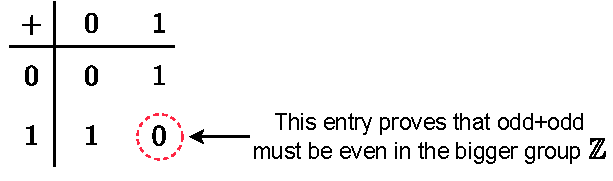
\includegraphics[width=0.65\textwidth]{Figures/Z2-cayley-example-later (1).pdf}

\end{example}

\begin{example}
$M\in GL_2(\R)= \{\text{inv }2\times 2's \text{ with }\R \text{ entries}\}$\steezybreak\\
\textit{Problem:} Show that $M=\begin{pmatrix}
r & 0 \\
0 & 1
\end{pmatrix}M'$ where $r\in \R-\{0\}$ and $det(M')=1$.\steezybreak\\
We'll use $SL_2(\R)=\{\det 1 \text{ matrices}\}\subset GL_2(\R)$.\steezybreak\\
\textit{Claim:} $SL_2(\R)\triangleleft GL_2(\R)$, we've already shown $SL_2(\R)<GL_2(R)$ so we only need to show that $SL_2(\R)$ absorbs conjugates.
\begin{align}
    \text{take }A, \text{ a matrix in } GL_2(\R) \text{ and } B \in SL_2(\R)\nonumber\\
    \det(ABA^{-1})=\det(A)\det(B)\det(A^{-1})=\det(A)(1)(\frac{1}{\det(A)}= (1)(1)=1 \nonumber \\
    \text{So } ABA^{-1}\in SL_2(\R) \nonumber \\
    \therefore SL_2(\R) \triangleleft GL_2(R) \nonumber 
\end{align}
So $GL_2(\R)/SL_2(\R)$ is a group.\steezybreak\\
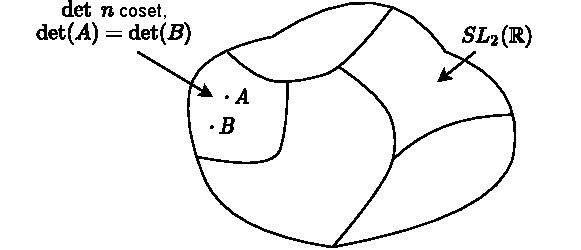
\includegraphics[width=0.5\textwidth]{Figures/aside_sl2(R).pdf}\steezybreak\\
Recall: The cosets are the equivalence classes under "$\equiv \mod H$".
\begin{align}
    A\equiv B \mod SL_2(\R) &\iff AB^{-1}\in SL_2(\R) \nonumber \\
    &\implies \det(AB^{-1})=1 \nonumber \\
    &\implies \det(A)\frac{1}{\det(B)}=1 \nonumber\\
    &\implies \det(A)=\det(B). \ \ \ \ \ \ \ \ \ \text{ (See figure.)}\nonumber 
\end{align}
For any choice of $n\in \R-\{0\}$, the $\det -n$ coset has a natural representative $\begin{pmatrix}
n & 0 \\
0 & 1
\end{pmatrix}$ so we have the $\det-n$ coset
\begin{align}
    \begin{pmatrix}
n & 0 \\
0 & 1
\end{pmatrix}SL_2(\R)\nonumber
\end{align}
Now, take $M\in GL_2(\R)$ and say $\det(M)=r$ ($r\neq 0$ because $M\in GL_2(\R)$), $M$ belongs to exactly one coset:
\begin{align}
    &\det-r \text{ class}:\nonumber\\
    &M\in \begin{pmatrix}
r & 0 \\
0 & 1
\end{pmatrix}SL_2(\R) \implies \exists \ M' \in SL_2(\R) \ni M= \begin{pmatrix}
n & 0 \\
0 & 1
\end{pmatrix}M'\nonumber
\end{align}
(Note $\det(M')=1$ since it is a member of  $SL_2(\R)$.)
\end{example}

\section{Homomorphisms}
\begin{definition}[Homomorphism]
$G,\bar{G}$ groups. A mapping $\phi: G\rightarrow \bar{G}$ is a \textit{homomorphism} if 
\begin{align}
    \phi(a \underset{\cdot \text{ in } G}{\cdot} b)=\phi(a)\underset{\cdot \text{ in } \bar{G}}{\cdot} \phi(b) \ \ \forall \ a,b\in G \nonumber
\end{align}
\end{definition}
Informally, we say $\phi: G \rightarrow \bar{G} $ is a homomorphism if it \textit{splits over products}.
\begin{figure}[h!]
    \centering
    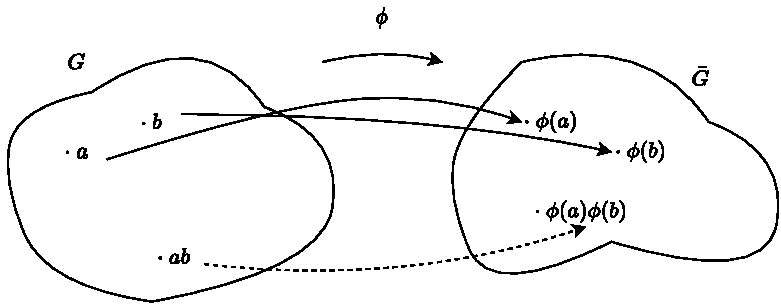
\includegraphics[width=0.85\textwidth]{Figures/homomorphisms_1.pdf}
    \caption{Visualizing A Homomorphism between Groups}
    \label{fig:morphism1fig}
\end{figure}

\begin{figure}[ht!]
    \centering
    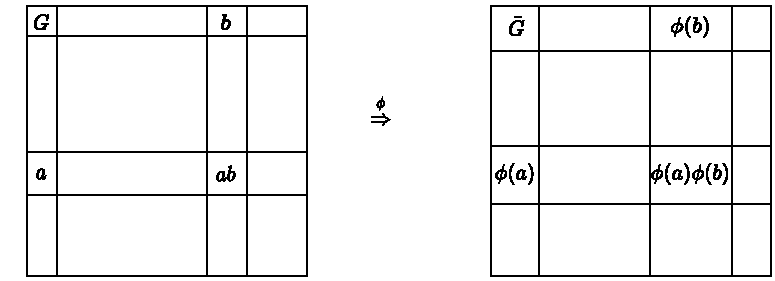
\includegraphics[width=0.85\textwidth]{Figures/homomorphisms_2 (1).pdf}
    \caption{Visualizing A Homomorphism between Groups}
    \label{fig:morphism2fig}
\end{figure}

\begin{figure}[h!]
    \centering
    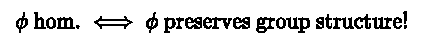
\includegraphics[width=0.55\textwidth]{Figures/homomorphisms_3 (1).pdf}
    \label{fig:morphism3fig}
\end{figure}
\newpage
\subsubsection{Some Examples of Homomorphisms}
\begin{example}
Trivial homomorphism:
\begin{align}
    &\phi: G\rightarrow \bar{G} \nonumber \\
    &\phi(x)=\ \underset{\in \bar{G}}{e} \ , \ \forall \ x\in G. \nonumber
\end{align}
Take $x,y\in G$
\begin{align}
    \phi(x)&=e \ \ (\text{by defn.}) \nonumber\\
    \phi(y)&=e \ \nonumber \\
    \phi(\ \underset{\in G}{xy}\ )&=e=e\cdot e =\phi(x)\cdot \phi(y). \nonumber\\
    &\therefore \phi \text{ is a homomorphism since it \textit{splits} over products.} \nonumber 
\end{align}
For the readers interested in category theory: In the category of groups (or of modules), a \textit{zero morphism} is a homomorphism $f : G \rightarrow \bar{G}$ that maps all of $G$ to the identity element of $\bar{G}$ (exactly the trivial homomorphism!). The zero object in the category of groups is the trivial group $1 = \{1\}$, which is unique up to isomorphism.
\end{example}
\begin{example}
Identity Homomorphism.
\begin{align}
    &\phi: G\rightarrow G \nonumber \\
    &\phi(x)=x, \ \forall \ x\in G \nonumber 
\end{align}
We can easily see this mapping splits over products, let $x,y\in G$:
\begin{align}
    \phi(x)&=x \nonumber \\
    \phi(y)&=y \nonumber \\
    \phi(xy)&=xy=\phi(x)\cdot \phi(y) \nonumber 
\end{align}
\end{example}

\begin{example}
Inclusion homomorphism: $H<G$, 
\begin{align}
    &\phi : H\rightarrow G \nonumber \\
    &\phi(h)= h \nonumber \ \forall h \in H \\
    \phi(h)&=h\in G, \ \ \phi(z)=z\in G \nonumber \\
    \phi(hz)&=hz\in G = \phi(h)\cdot \phi(z) \nonumber
\end{align}
"Inclusion" is a shift in perspective.
\end{example}

\begin{example}
Conjugation by $g\in G$.
\begin{align}
    \text{fix } &g \in G. \nonumber \\
    &\phi_g: G\rightarrow G \nonumber \\
    &\phi_g(x)=gxg^{-1} \ \forall \ x \in G \nonumber \\
    \phi_g(xy)=gxyg^{-1}&=gxeyg^{-1}=gx(g^{-1}g)yg^{-1} \nonumber \\
    &=(gxg^{-1})(gyg^{-1}) \nonumber \\
    &=\phi_g(x)\cdot \phi_g(y). \nonumber \\
    \therefore \phi_g \text{ is a homomorphism on }G. \nonumber 
\end{align}
\end{example}

\begin{example}
Determinant
\begin{align}
    G&=GL_2(\R) \ \text{ under matrix multiplication} \nonumber \\
    \bar{G}&=\R-\{0\} \ \text{ under multiplication } \nonumber \\
    &\phi:G\rightarrow \bar{G} \nonumber\\
    \text{ defined by } &\phi(M)=\det(M) \nonumber\\
    \phi(MN)=\det(MN)&=\det(M)\det(N)=\phi(M)\phi(N) \nonumber 
\end{align}
\end{example}

\begin{example}
Evaluation map.
\begin{align}
    &G= \{\text{real-valued mappings: } \R \rightarrow \R \} \text{ under }+ \nonumber \\
    \text{Let }&f,g,h:\R \rightarrow \R \nonumber \\
    &(f+g)+h=f+(g+h) \ \ \ \ \ e\text{ is }f(x)=0 \ \ \ \ \ [f(x)]^{-1}=-f(x) \nonumber \\
    &\text{Now let } \bar{G} = \R \text{ under }+ \nonumber \\
    &\text{fix }r\in \R \nonumber \\
    &\text{Define } \phi_r:G\rightarrow \bar{G} \text{ by } \phi_r(f(x))=f(r) \nonumber \\
    &\text{ Take } f(x),g(x)\in G \nonumber \\
    &\phi_r[f(x)\cdot g(x)]=(f+g)(r)=\underset{\in \R}{f(r)+g(r)} = \phi_r(f(x))+\phi_r(g(x)) \nonumber
\end{align}
\end{example}

\textit{More examples of Homomorphisms can be found in Herstein's Topics in Algebra 2 ed.  pgs. 55-56}\steezybreak\\

\begin{lemma}
$N\triangleleft G$,
\begin{align}
    \text{Define } &\phi: G\rightarrow G/N  \ \ \ \ (\text{Remember: }G/N \text{ is the set of cosets of } N \text{ in }G ) \nonumber \\
    \text{by } &\phi(g)=Ng \ \ \forall g \in G \nonumber
\end{align}
Then $\phi$ is a surjective homomorphism, called the "canonical" or "natural" map. \\
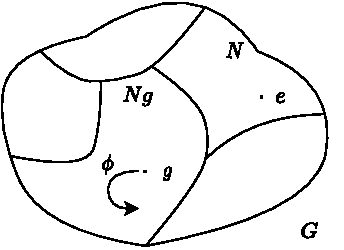
\includegraphics[width=0.45\textwidth]{Figures/natural_map.pdf}This map takes $g\in G$ to the coset in which it sits. \\

\noindent\textit{Proof:}
\begin{align}
    &\text{Let }g,g'\in G \nonumber \\
    &\phi(g\cdot g')= N(g\cdot g')\underset{\cdot \text{ in }G/N}{=} NgNg' = \phi(g)\cdot \phi(g'). \nonumber \\
    &\therefore \ \phi \text{ is a homomorphism.} \nonumber
\end{align}
$\phi$ is surjective: \\
\begin{align}
    \text{Let }Nx \in G/N \ \ \ (\text{i.e. } Nx \text{ is a random coset}) \nonumber \\
    \phi(x)=Nx \nonumber
\end{align}
so $x$ serves as a pre-image for $Nx$. $\blacksquare$
\end{lemma}


\begin{lemma}
Given $\phi: G\rightarrow \bar{G}$ a homomorphism,
\begin{enumerate}[label=\roman*)]
    \item $\phi(e)=\bar{e}$
    \item $\phi(g^{-1})=[\phi(g)]^{-1}$
\end{enumerate}
\textit{Proof:}
\begin{enumerate}[label=\roman*)]
    \item \begin{align}
        &\phi(e)\cdot \bar{e}=\phi(e)=\phi(e\cdot e)=\phi(e)\cdot\phi(e) \nonumber \\
        \implies & \not {\phi(e)}\cdot \bar{e}=\not{\phi(e)}\cdot\phi(e) \ \ \ \ \text{by left cancellation of $\phi(e)$ in }\bar{G} \nonumber \\
        \implies &\bar{e}=\phi(e) \nonumber
    \end{align} 
    \item Inverses. Take $g\in G$, $\phi(g)$ has a unique inverse in $\bar{G}$. We will show $\phi(g^{-1})$ satisfies inverse property
    \begin{align}
        &\phi(g^{-1})\cdot \phi(g)= \phi(g^{-1}\cdot g)=\phi(e)=\bar{e} \nonumber \\
        &\phi(g)\cdot\phi(g^{-1})=\phi(g\cdot g^{-1})=\phi(e)=\bar{e} \nonumber
    \end{align}
    So $\phi(g^{-1})=[\phi(g)]^{-1}$\\
    Since $\phi(g^{-1})$ does the job of an inverse and inverses must be unique, $\phi(g^{-1})$ is the unique inverse of $\phi(g)$. $\blacksquare$ 
\end{enumerate}
\end{lemma}
\newpage
\begin{definition}[Kernel]
Let $\phi:G\rightarrow \bar{G}$ be a homomorphism. The \textit{kernel} of $\phi$ is the set of elements in $G$ that $\phi$ sends to the identity element in $\bar{G}$
\begin{align}
    K= \{g\in G | \phi(g)=\bar{e}\}. \nonumber
\end{align}
Note, $K\neq \{\}$ because $e\in K$ by L 2.7.2 (i). $K$ is also commonly denoted ``$\text{ker}\ \phi$" or ``$\text{ker}(\phi)$" to avoid ambiguity when there are multiple homomorphisms being discussed.\\
\begin{center}
    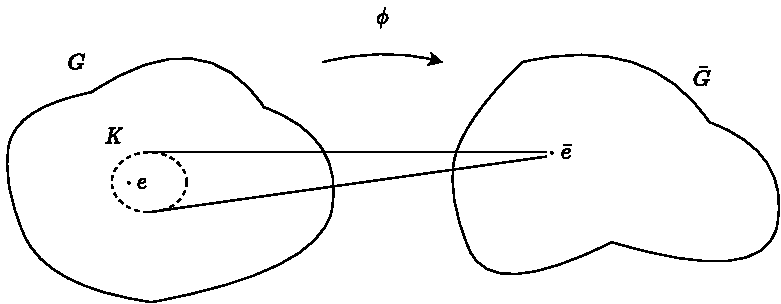
\includegraphics[width=0.65\textwidth]{Figures/kernel_hom.pdf}
\end{center}
\end{definition}

\begin{lemma}
$\phi:G\rightarrow \bar{G}$ hom. with kernel $K$. Then $K\triangleleft G$. \steezybreak\\

\noindent \textit{Proof:} We know $e\in K$ so $K$ is non-empty and L 2.4.1 applies (we begin by showing $K<G$ then to show 'normal' part we will show $K$ absorbs conjugates).
\begin{enumerate}[label=\roman*)]
    \item Closure. Let $a,b\in K$
    \begin{align}
        &\phi(ab)\underset{\phi \text{ hom.}}{=}\phi(a)\phi(b)\underset{a,b\in K}{=} \bar{e}\bar{e}=\bar{e} \nonumber \\
        &\therefore ab\in K. \nonumber 
    \end{align}
    \item Inverses. Let $a\in K$  (remember $a\in G \implies a^{-1}\in G$)
    \begin{align}
        &\phi(a^{-1})=[\phi(a)]^{-1}=[\bar{e}]^{-1}=\bar{e}\nonumber \\
        &\therefore a^{-1}\in K. \nonumber 
    \end{align}
\end{enumerate}
By Lemma 2.4.1 $K<G$. \\
Now to show that $K$ is normal we will show it absorbs conjugates. Take $x\in K$ and $g\in G$.
\begin{align}
    \phi(gxg^{-1})&= \phi(g)\phi(x)\phi(g^{-1}) = \phi(g)\bar{e}\phi(g^{-1})\nonumber \\
    &= \phi(g)\phi(g^{-1})=\phi(g\cdot g^{-1})= \phi(e)=\bar{e}. \nonumber
\end{align}
Since $gxg^{-1}\in K$, $K\triangleleft G$. $\ \ \blacksquare$
%\textit{This proof is incomplete, will finish later today}
\end{lemma}

\begin{proposition}
$\phi:G\rightarrow \bar{G}$ hom. with kernel $K$.
\begin{align}
    \phi \text{ is injective } \iff K= \{e\}\nonumber
\end{align}
\textit{Proof:}\\
$\Rightarrow \ :$ Assume $\phi$ injective.\\
\begin{align}
    \text{Take }k\in K \nonumber \\
    \phi(k)=\bar{e}=\phi(e) \nonumber \\
    \text{If }k\neq e , \phi \text{ inj. } \implies \phi(k)\neq \phi(e)\ ...\ \Rightarrow \Leftarrow \nonumber \\
    \therefore k \text{ must be }e; \ K=\{e\} \nonumber
\end{align}
$\Leftarrow \ :$ Assume $K=\{e\}$.\\
Injective means distinct elements stay distinct. We will use contraposition to show $\phi$ is injective. \steezybreak\\ %(i.e. rather than show $A\implies B$ is true we will show the equivalent contraposition $\lnot B \implies \lnot A$ is true). \\
(i.e. we want to show $a\neq b \implies \phi(a)\neq \phi(b)$ so we will equivalently show $\phi(a)=\phi(b) \implies a= b$ which is the contraposition of the desired implication.)\steezybreak\\
By contrapositive: if 2 images are not distinct, then their pre-images are not distinct. Consider:
\begin{align}
    \phi(g_1)=\phi(g_2)\nonumber
\end{align}
Now left multiplying by $[\phi(g_1)]^{-1}$
\begin{align}
    \bar{e}&=[\phi(g_1)]^{-1}\phi(g_2)\nonumber \\
    &= \phi(g_1^{-1}g_2) \nonumber \\
    &\therefore g_1^{-1}g_2\in K \nonumber
\end{align}
now since $K=\{e\}\ \ \implies g_1^{-1}g_2=e \implies g_1=g_2$\\
$\therefore \ \phi$ is injective. $\ \ \blacksquare$
%\textit{This proof is incomplete, will finish later today}
\end{proposition}

Let's have a look at calculating Kernels of homomorphisms.
\begin{example}
Fix $g\in G$ and define $\phi_g: G\rightarrow G$ by $\phi_g(x)=gxg^{-1}\ \forall \  x \in G$. \\
Now, take $k\in K$.
\begin{align}
    \phi_g(k)=e=gkg^{-1} \nonumber
\end{align}
solve for $k$
\begin{align}
    g&=gk\nonumber \\
    g^{-1}g&=k\nonumber \\
    e&=k\nonumber 
\end{align}
$\therefore K = \{e\}$, so $\phi_g$ is injective by the proposition above.
\end{example}

\begin{example}
$\phi:\overset{\text{mat. mult.}}{GL_n(\R)}\rightarrow \overset{\text{mult.}}{\R-\{0\}}$ \\
$\phi(M)=\det(M)$. \\
Suppose $M\in \ker(\phi)$, then
\begin{align}
    \phi(M)=\det(M)=1 \nonumber
\end{align}
So $M\in \ker(\phi) \iff \det(M)=1$ which means
\begin{align}
    \ker(\phi)&=\{n\times n \text{ matrices with entries in }\R \text{ having determinant }1\}\nonumber \\
    &=SL_n(\R) \neq \{I_n\} \nonumber
\end{align}
$\therefore \phi$ is \textit{not} injective.
\end{example}

\begin{example}
Fix $r\in \R$. \\
Consider $\phi_r: \{\text{real valued functions }\}\rightarrow \R$ defined by
\begin{align}
    \phi_r(f)=f(r)\nonumber
\end{align}
If $f\in \ker(\phi_r)$ then $\phi_r(f)=0$ since $0$ is the "$e$" in $\R$ under $+$. \\
So $\ker(\phi_r) = \{\text{set of functions with root at } r\} \neq \{f(x)=0\}$ so $\phi_r$ is \textit{not} injective.
\end{example}

\begin{example}
Assume $N\triangleleft G$ and consider again the $\phi$ from Lemma 2.7.1 going from $G$ to the group of cosets of $N$ in $G$, $G/N$:
\begin{align}
    \phi: G\rightarrow G/N \nonumber \\
    \phi(g)= Ng \nonumber
\end{align}
What is $\ker(\phi)$ in this case? If $g\in \ker(\phi)$ then
\begin{align}
    \phi(g)=e= N \ \ \ \text{(Remember, $N$ is the $e$ in $G/N$)}\nonumber \\
    Ng=\phi(g)=N \nonumber
\end{align}
$g$'s coset is $N$. So every element of $N$ is in $\ker(\phi)$.\\
$\therefore \ \ker(\phi)=N$. 
\end{example}

\begin{definition}[Image of Group under a Homomorphism]
$\phi: G\rightarrow \bar{G}$ group hom., then 
\begin{align}
    \phi(G)= \{\phi(g)\ | \ \forall g\in G\}\nonumber
\end{align}
is the \textit{image of }$G$ \textit{under} $\phi$.\steezybreak\\
Note that $\phi(G)=\bar{G}\iff \phi \text{ is surjective (onto)}$. Prove this as an exercise.
\end{definition}
\begin{proposition}
$\phi:G\rightarrow \bar{G}$ group hom.\steezybreak\\
Then $\phi(G)< \bar{G}$\steezybreak\\
\textit{Proof:} $\phi(G)$ is non-empty since $\phi(e)=\bar{e}\in \phi(G)$ so L 2.4.1 applies
\begin{enumerate}[label=\roman*)]
    \item Closure: take $y,y'\in \phi(G)$, then
    \begin{align}
        \text{there exists } &x,x'\in G \ni \phi(x)=y \text{ and } \phi(x')=y' \nonumber \\
        &xx'\in G \text{   , since } G \text{ is a group.} \nonumber \\
        &\phi(xx')=\phi(x)\phi(x')=yy' \nonumber \\
        \therefore \ &yy'\in \phi(G) \nonumber
    \end{align}
    \item Inverses: Take $y\in \phi(G), \ \implies \exists \ x\in G \ni \phi(x)=y$\\
    \begin{align}
        &y^{-1}=[\phi(x)]^{-1}=\phi(x^{-1})\nonumber\\
        &x^{-1}\in G \text{   , since } G \text{ is a group,} \nonumber \\
        \therefore \ &y^{-1}\in \phi(G). \ \ \ \ \ \ \blacksquare \nonumber
    \end{align}
\end{enumerate}
\end{proposition}

\begin{tcolorbox}
    $\star$ \textbf{Important Note:} A homomorphism $\phi: G\rightarrow \bar{G}$ that is not surjective can be redefined so that it is surjective like this:\\
    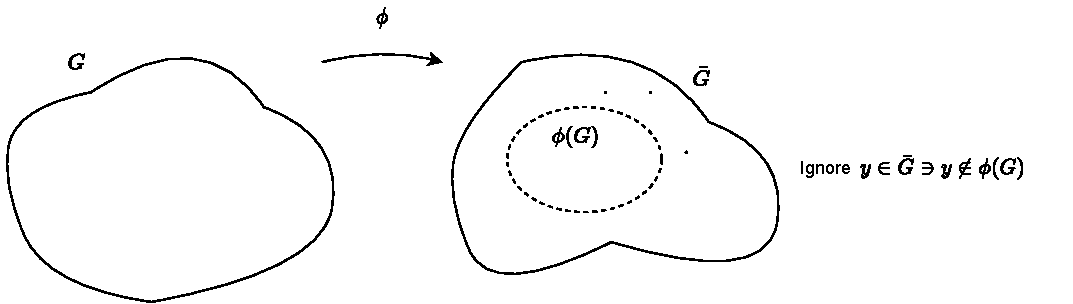
\includegraphics[width=\textwidth]{Figures/make_surj1.pdf}\\
    i.e. discard non participants in the map. We can toss these out with no effect on the map.\\
    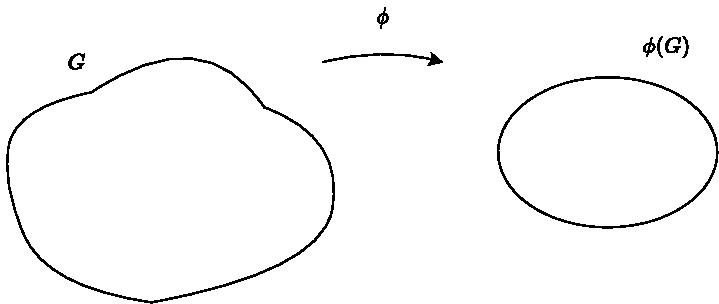
\includegraphics[width=0.7\textwidth]{Figures/make_surj3.pdf}\\
    Instead of $\phi:G\rightarrow \bar{G}$; redefine as $\phi: G\rightarrow \phi(G)$ so now $\phi$ is surjective.
\end{tcolorbox}

\begin{definition}[Isomorphism]
An \textit{isomorphism} between groups is a bijective homomorphism. \steezybreak\\
$G$ and $G^*$ are isomorphic groups, denoted $G\approx G^*$ (or often $G\simeq G^*$, though we prefer the former convention) if $\exists$ an isomorphism from $G$ to $G^*$.
\begin{align}
    G\approx G^* \iff \exists \ \sigma: G\rightarrow G^* \ni 
    \begin{cases}
      \sigma \text{ is a homomorphism}\\
      \sigma \text{ is injective}\\
      \sigma \text{ is surjective}
    \end{cases} \nonumber 
\end{align}
\end{definition}
some day I will type up handout 3 but for now look at it while you read along, the $\tilde{G}$ is a subgroup of $G_{17}$. Let's have a look at $\Z_8$
\begin{align}
    \Z_8=\langle 1 \rangle =\langle 3 \rangle = \{3^n\ | \ n\in \Z \} \ (\text{Remember, }\Z_8\text{'s group operation is } + \text{ mod }8).\nonumber\\
    \tilde{G}=\langle 2 \rangle = \{2,4,8,16,15,...,1\}=\langle 8 \rangle = \{8^n\ | \ n\in \Z\} \ (\text{Remember, }G_{17}\text{'s group operation is } \times \text{ mod }17).\nonumber
\end{align}
\newpage
\begin{multicols}{2} % two columns
        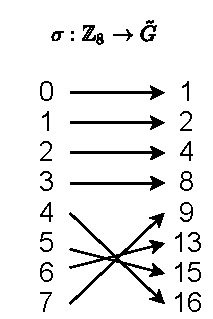
\includegraphics[width=0.35\textwidth]{Figures/iso_example_Z8_G17.pdf} 
        
        To show that $\Z_8 \approx G_{17}$ we will construct a mapping $\sigma$ from $\Z_8$ to $G_{17}$ that is a homomorphism and is a bijection. To show the first property we show that $\sigma$ splits over products for generators of each of the groups which is sufficient to show it splits for all products. 
        \begin{enumerate}
            \item $\sigma(3^n)=8^n$\\
            $\sigma(3^m 3^n)= \sigma(3^{m+n})=8^{m+n}=8^m8^n=\sigma(3^m)\sigma(3^n), \ \ \therefore \sigma $ hom.
            \item From the figure the homomorphism we have defined is obviously a 1-1 correspondence so $\sigma$ is a bijection. %(if this isn't obvious to you, convince yourself with the diagram that every unique element in $\tilde{G}$ has preimage in $\Z_8$ (surjective) and that each of those images are unique meaning if $z\neq y$ then $\phi(z)\neq \phi(y)$ (injective)).
        \end{enumerate}
        $1 \ \& \ 2$ together $\implies $ $\sigma$ is an isomorphism.
\end{multicols}

\noindent$\boxed{\textbf{Important Fact:}}$ Any two cyclic groups of the same order are isomorphic.\\
This is true via the map $\phi: \langle a\rangle \rightarrow \langle b \rangle $ (Where $a$ is the generator of one group and $b$ the generator of another) defined by $\phi(a^n)=b^n$, note that the Law of Exponents for groups implies that $\phi$ is a homomorphism. It can be easily checked that $\phi$ is a bijection. \steezybreak\\

\begin{corollary}
If $G$ is cyclic of order $n$, then $G$ is isomorphic to $\Z_n$.\\
\begin{align}
    G\approx \Z_n . \ \ \leftarrow (\text{ Note that }\Z_n \text{ is cyclic generated by } 1.)\nonumber
\end{align}
\end{corollary}

\begin{proposition}
$\approx$ is an equivalence relation on the set of all groups (finite).\\
\textit{Proof:} We need to show that $\approx$ is reflexive, symmetric, and transitive.
\begin{enumerate}
    \item Reflexive: $G\approx G$ via the identity map
    \item Symmetric: Assume $G\approx G^*$. This means $\exists$ bijective homomorphism $\sigma: G\rightarrow G^*$. By Lemma 1.2.3 $\sigma$ is bijective $\iff$ $\sigma$ has an inverse mapping $\sigma^{-1}$. So $\exists$ $\sigma^{-1}: G^*\rightarrow G$ which satisfies
    \begin{align}
        \sigma^{-1}\circ \sigma &= I_G \nonumber \\
        \sigma\circ \sigma^{-1}&=I_{G^*}\nonumber
    \end{align}
    Note that $(\sigma^{-1})^{-1}=\sigma $, so $\sigma^{-1}$ has an inverse mapping (namely $\sigma$) so $\sigma^{-1}$ is a bijection.\\
    \textit{Claim:} $\sigma^{-1}$ is a homomorphism: take $x^*,y^*\in G^*$
    \begin{align}
        \sigma \text{ surj. } \implies \ \exists x\in G \ni \sigma(x)=x^* \ \text{ and} \nonumber \\
        \sigma^{-1}(x^*)=\sigma^{-1}(\sigma(x))=I_G(x)=x \nonumber
    \end{align}
    Similarly,
    \begin{align}
        \sigma \text{ surj. }&\implies \ \exists y\in G \ni \sigma(y)=y^* \nonumber \\
        \sigma^{-1}(x^*y^*)&=\sigma^{-1}(\sigma(x)\sigma(y))\underset{\sigma \text{ hom.}}{=}\sigma^{-1}(\sigma(xy))=xy=\sigma^{-1}(x)\sigma^{-1}(y) \nonumber \\
        &\therefore \sigma^{-1} \text{ is a bijective hom.} \nonumber \\
        &\therefore G^*\approx G, \approx \text{ is symmetric}. \nonumber
    \end{align}
    \item Transitive: Assume $G\approx G^*$ and $G^*\approx \bar{G}$
    \begin{align}
        G\approx G^* &\implies \ \exists \ \sigma: G\rightarrow G^* \ \text{ Bijective hom.} \nonumber \\
        G^*\approx \bar{G} &\implies \ \exists \ \tau: G^* \rightarrow \bar{G} \ \text{ also Bijective hom.}\nonumber
    \end{align}
    Then $\tau \circ \sigma: G\rightarrow \bar{G} $ is a bijection by L.1.2.2 (composition of mappings). We claim that, moreover, $\tau \circ \sigma$ is a homomorphism:\\
    Take $x,y\in G$
    \begin{align}
        (\tau \circ \sigma) (xy)&=\tau(\sigma(xy))\underset{\sigma \text{ hom.}}{=}\tau(\sigma(x)\underset{\cdot \text{ in } G^*}{\cdot}\sigma(y)) = \tau(\sigma(x))\underset{\cdot \text{ in } \bar{G}}{\cdot} \tau(\sigma(y))\nonumber \\
        &=(\tau \circ \sigma)(x)\cdot (\tau\circ \sigma)(y) \nonumber \\
        &\therefore \tau\circ \sigma \text{ is a homomorphism.} \nonumber\\
        &\therefore \tau\circ \sigma \text{ is a bijective hom. }\implies \text{ Isomorphism} \nonumber \\
        &\therefore G\approx \bar{G}, \text{ so } \approx \text{ is transitive.} \ \ \blacksquare \nonumber
    \end{align}
\end{enumerate}
\end{proposition}

\begin{figure}
    \centering
    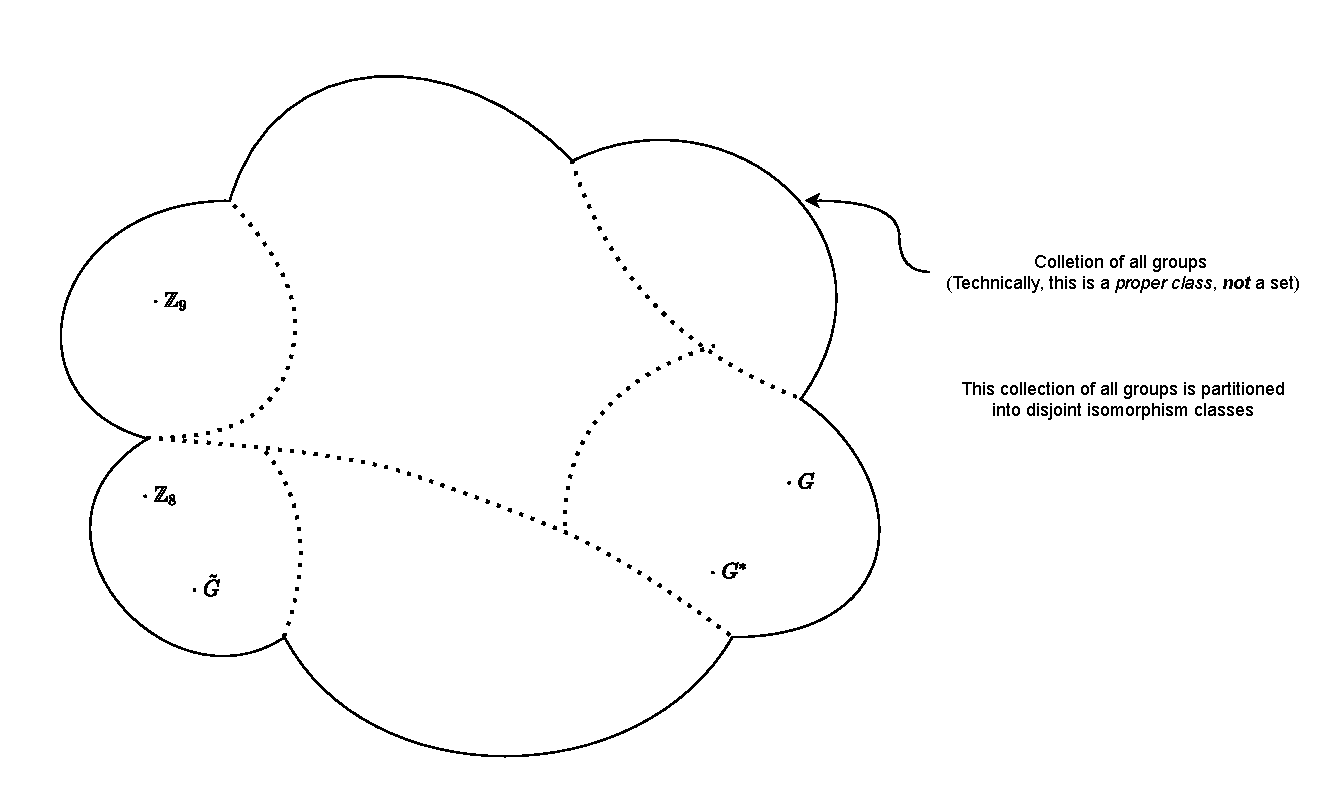
\includegraphics[width=\textwidth]{Figures/ClassofGroups_part (1).pdf}
    \caption{Collection of All Groups is a Proper Class, Isomorphism partitions this class into disjoint isomorphism classes}
    
    \label{fig:my_label}
\end{figure}
\subsection*{Some Ways that Groups fail to be Isomorphic}
\begin{enumerate}
    \item Different Orders
    \item One is cyclic, other is not.
    \item One is abelian, other is not.
    \item Different subgroup lattices
    \item Different order tables
    \item Different \# of Squares
\end{enumerate}
\begin{tcolorbox}
    \begin{center}
        $\star\star\star$ \textbf{Read up to this point to Complete Homework 5} $\star\star\star$
    \end{center}
    \end{tcolorbox}
\newpage
\setcounter{dummy}{0}
\begin{theorem}[The First Isomorphism Theorem] 
If $\phi$ is a surjective group homomorphism from $G$ to $\bar{G}$ with kernel $K$, then
\begin{align}
    G/K\approx \bar{G} \nonumber
\end{align}
\textit{Proof:}\\
$K\triangleleft G \implies G/K$ is a quotient group (consisting of cosets of $K$ in $G$, $KxKy=Kxy$). We learn about $\bar{G}$ by studying $G/K$. Recall the canonical map from Lemma 2.7.1,
\begin{align}
    \sigma : G \rightarrow G/K \nonumber \\
    \sigma(g)=Kg \nonumber
\end{align}
Now, to show $G/K$ and $\bar{G}$ are isomorphic we must demonstrate that there exists a bijective homomorphism between them. We want a $\tau$ like the one in the diagram below.\steezybreak\\

\noindent Here's the situation: \\
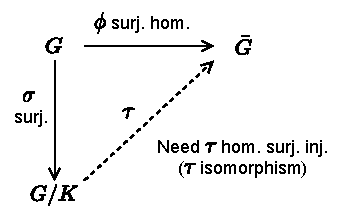
\includegraphics[width=0.5\textwidth]{Figures/1stiso_diag1.pdf} \\
Define $\tau: G/K \rightarrow \bar{G}$ as follows, $\tau(Kg)=\phi(g)$, is $\tau$ well-defined? (i.e. is $\tau$ a mapping?)\steezybreak\\
Potential problem: $Kg$ can have more than one preimage under $\sigma$.\\
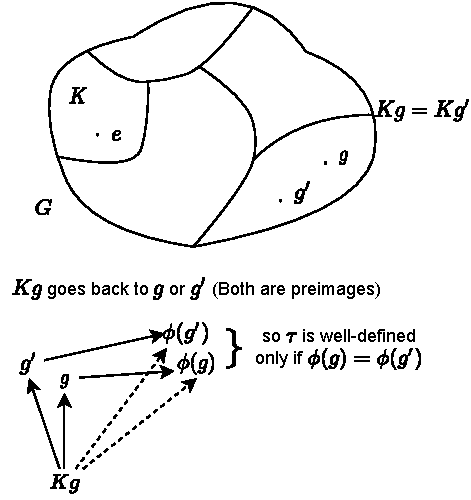
\includegraphics[width=0.5\textwidth]{Figures/1stIso_diag2.pdf}\\
\begin{align}
    \text{Assume }&Kg=Kg' \nonumber \\
    &g'\in Kg'=Kg \nonumber \\
    &\therefore \exists \ k\in K \ni g'=kg \nonumber \\
    \phi(g')&=\phi(kg)=\phi(k)\phi(g)=\bar{e}\phi(g)=\phi(g). \nonumber
\end{align}
Kernel is necessary coset. \\
$\therefore$\\
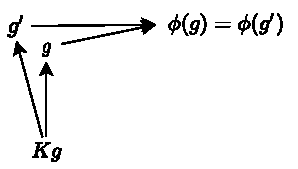
\includegraphics[width=0.45\textwidth]{Figures/1stIso_diag3.pdf} \\
$\therefore \ \tau$ is well-defined. \\
Now it remains to show that $\tau$ is a homomorphism and is bijective. 
 
\textbf{$\tau$ homomorphism:}\\
\begin{align}
    &\tau : G/K \rightarrow \bar{G}, \text{ take } Kg,Kh\in G/K \nonumber \\
    &\tau(KgKh)=\tau(Kgh)=\phi(gh)=\phi(g)\phi(h)= \tau(Kg)\tau(Kh). \nonumber
\end{align} 
So $\tau$ is a homomorphism.\\
To show that $\tau$ is a bijection we will use Lemma 1.2.3 and show that $\tau$ has an inverse mapping. \\
\begin{align}
    &\text{Define }\mu : \bar{G}\rightarrow G/K \text{ by }\nonumber \\
    &\mu(\bar{g})=Kg \ \text{Where }g\text{ is a preimage for }\bar{g} \text{ under }\phi, \text{  (think of $\bar{g}$ as $\phi(g)$)} \nonumber
\end{align}
Is $\mu$ well-defined? We know at least one preimage exists because $\phi$ is surjective by assumption... what if $\bar{g}$ has more than one preimage?
\begin{align}
    \text{Assume } \bar{g}=\phi(g)=\phi(h) \nonumber
\end{align}
Is $Kg=Kh$?
\begin{align}
    \phi(g)&=\phi(h) \nonumber \\
    \implies \phi(g)[\phi(h)]^{-1}&=\bar{e} \nonumber \\
    \implies \phi(g)\phi(h^{-1})&=\bar{e} \nonumber \\
    \implies \phi(gh^{-1})&=\bar{e} \nonumber \\
    \therefore gh^{-1}\in K = \ker\phi \nonumber
\end{align}
Now $gh^{-1} \in K$ implies both $g\in Kg$ (since $e\in K$) and $g\in Kh$ (since $gh^{-1} \in K$ and $gh^{-1}h\in Kh$), therefore $Kg=Kh$ (They must be identical since they are not disjoint, since cosets are equivalence classes)\\
$\therefore \ \mu$ is well-defined 
\begin{align}
    (\tau \circ \mu)(\bar{g})=\tau(\mu(\bar{g}))=\tau(Kg)=\phi(g)=\bar{g} \nonumber \\
    \therefore \ (\tau\circ\mu)= I_{\bar{G}} \nonumber \\
    (\mu \circ \tau)(Kg)=\mu(\tau(Kg))=\mu(\phi(g))=Kg \nonumber \\
    \therefore (\mu\circ\tau)=I_{G/K} \nonumber
\end{align}
So $\tau$ has an inverse $\mu$ making $\tau$ a bijective homomorphism (Isomorphism).
\begin{align}
    \therefore G/K \approx \bar{G} \ \text{ via } \tau \ \ \ \ \ \ \blacksquare \nonumber
\end{align}
%This proof is incomplete, will finish soon, though you should be able to see where this is headed :) we will use the canonical map from L 2.7.1 and use this map to define another map which is a bijective homomorphisms from $G/K$ to $\bar{G}$ ( we first have to construct it an show its well-defined (is a mapping))
\end{theorem}

\subsection*{$H<G$, Some Easy ways to tell if $H\triangleleft G$}
Recall
\begin{align}
    H\triangleleft G &\iff ghg^{-1}\in H \ \forall \ g\in G, \forall \ h\in H \nonumber \\
                     &\iff gH=Hg \ \forall \ g\in G \nonumber \\
                     &\underset{L 2.6.2}{\iff} gHg^{-1}=H \ \forall \ g\in G. \nonumber
\end{align}
\begin{enumerate}
    \item (Trivials) $G\triangleleft G$ because $g\hat{g}g^{-1}\in G$ by closure of $G$. $\{e\}\triangleleft G$ because $geg^{-1} \in \{e\} \ \forall \ g\in G$.
    \item Useful fact (after Lemma 2.6.2): $H<G$, $i_G(H)=2$, then $H\triangleleft G$ and $\frac{o(G)}{o(H)}=2\implies o(H)=\frac{1}{2}o(G)$
    \item \begin{enumerate}[label=\roman*)]
        \item $Z(G)\triangleleft G$ (Homework \#5)
        \item $H<Z(G) \implies H\triangleleft G$
        \begin{align}
            ghg^{-1}=gg^{-1}h=h\in H \nonumber
        \end{align}
        \item $G$ abelian $\implies $ every subgroup of $G$ is normal in $G$.\\
        \begin{align}
            Z(G)=G \ \ \text{(use (ii))}\nonumber
        \end{align}
    \end{enumerate}
    \item If $H$ is the only subgroup of its order $\subset G$, then $H\triangleleft G$.\\
    \textit{Proof:} Fix $g\in G$\\
    \textbf{Claim 1:} $gHg^{-1}< G$, first we note that $e\in H$ so $geg^{-1}\in gHg^{-1}$, therefore $gHg^{-1}$ is non-empty and so Lemma 2.4.1 applies.
    \begin{enumerate}
        \item Closure: $ghg^{-1},gh'g^{-1} \in gHg^{-1}$, \\
        \begin{align}
            (ghg^{-1})(gh'g^{-1})=g \underset{\in H}{(hh')}g^{-1} \in gHg^{-1}.\nonumber
        \end{align}
        \item Inverses: 
        \begin{align}
            (ghg^{-1})^{-1}=(g^{-1})^{-1}h^{-1}g^{-1}=g\underset{\in H}{h^{-1}}g^{-1} \in gHg^{-1} \ \ \ \ \blacksquare \ \ \ \ \text{(Claim 1 Proven)}\nonumber
        \end{align}
    \end{enumerate}
    \textbf{Claim 2:} $o(gHg^{-1})=o(H)$\steezybreak\\
    \begin{align}
        \text{Define } &\sigma:H\rightarrow gHg^{-1} \nonumber \\
        &\sigma(h)=ghg^{-1} \nonumber 
    \end{align}
    To show $\sigma$ is a bijection we'll show $\sigma^{-1}$ exists (L 1.2.3). 
    \begin{align}
        \text{Define } \mu:gHg^{-1} \rightarrow H \nonumber \\
        \mu(ghg^{-1})=g^{-1}(ghg^{-1})g =h \nonumber
    \end{align}
    operations make $\mu$ well-defined. Now we will show $\mu=\sigma^{-1}$.
    \begin{align}
        (\mu \circ \sigma)(h)=\mu(\sigma(h))=\mu(ghg^{-1})=h\nonumber \\
        \text{so }(\mu\circ \sigma)=I_H\nonumber \nonumber \\
        (\sigma\circ \mu)(ghg^{-1})=\sigma(\mu(ghg^{-1}))=\sigma(h)=ghg^{-1} \nonumber\\
        \text{so }(\sigma \circ \mu )=I_{gHg^{-1}}\nonumber
    \end{align}
    $\therefore \ \mu=\sigma^{-1}$ so $\sigma$ is a bijection.\\
    So there is a one-to-one correspondence between $gHg^{-1}$ and $H$ so $o(gHg^{-1})=o(H)$. But $H$ is the only subgroup of $o(H)$, $\therefore gHg^{-1}=H$.
    %\textit{This proof is incomplete, it will be finished very soon!!}
    \item For $H<G$ that don't fit the above criteria (shortcuts 1-4) we can always just check conjugates. Recall that $H\triangleleft G \iff ghg^{-1} \in H \ \forall \ h \in H$ and $\forall \ g \in G$, we now present shortcut \# 5. \steezybreak\\
    In checking conjugates, it suffices to check generators \textit{only}, because all elements are built from generators. For example: Let $G=\langle a,b \rangle$ $H= \langle x,y \rangle$. Then we must check: $axa^{-1}$, $bxb^{-1}$, $aya^{-1}$, $byb^{-1} \ \ \in H$? \steezybreak\\
    If each one of these is $\in H$, then $H\triangleleft G$ because all other conjugates reduce to products...\\
    for example $xy\in H$, $ab\in G$\\
    \begin{align}
        (ab)xy(ab)^{-1}&=abxyb^{-1}a^{-1} \nonumber \\
        &=a\underbrace{\underbrace{bxb^{-1}}_{\in H}\underbrace{byb^{-1}}_{\in H}}_{\in H }a^{-1} \ \ (\text{ so it's built from $x$ and $y$; say it's $x^2y$ for simplicity})\nonumber \\
        &= ax^2ya^{-1} \nonumber \\
        &= axxya^{-1} \nonumber \\
        &= \underbrace{axa^{-1}}_{\in H} \underbrace{axa^{-1}}_{\in H} \underbrace{aya^{-1}}_{\in H} \in H \nonumber
    \end{align}
    \item To show $H \not \triangleleft \ G$, give specific $g\in G$ and $h\in H$ for which $ghg^{-1}\not\in H$.
\end{enumerate}

\section{Dihedral Groups}
\textit{Exercise ( From Herstein P. 54 \# 17)}\\
\begin{definition}[Dihedral Group]
$n\in \Z, \ n \geq 3$. The \textit{Dihedral Group} denoted $D_n$ consists of rotations and reflections in the plane which send a regular $n-$gon centered at $(0,0)$ to itself. $D_n$ is also known as the \textit{symmetry group} of the $n$-gon.
\end{definition}
\begin{example}
\begin{align}
    D_3 & \ \ \ \ \text{ (symmetry group of triangle)}\nonumber \\
    &= \{ \text{rotations and reflections which send a regular tri-gon to itself} \} \nonumber
\end{align}
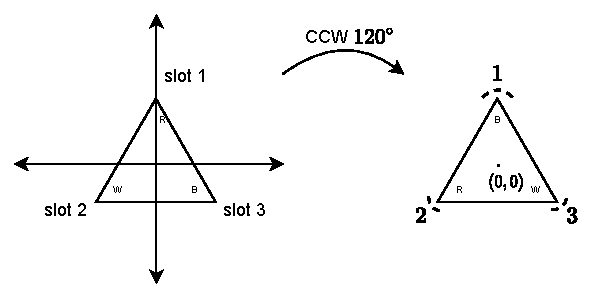
\includegraphics[width=0.75\textwidth]{Figures/Dihedral Group Example_1.pdf}

\hspace{-0.5in}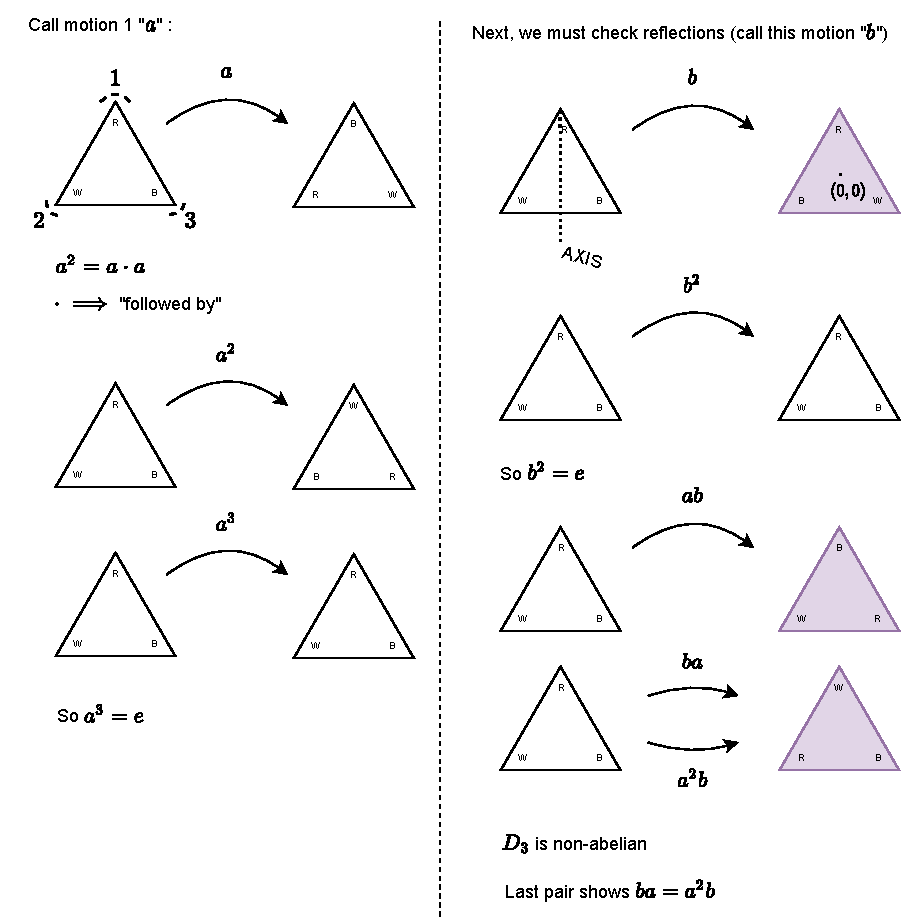
\includegraphics[width=1.1\textwidth]{Figures/Dihedral Group Example_2.pdf}\\
\begin{align}
    D_3&= \{e,a,a^2,b,ba,ab\} \nonumber \\
    &= \langle \underbrace{a}_{*},\underbrace{b}_{**} \rangle \nonumber \\
    &* - \text{ Rotation through }120^\circ \text{ CCW.} \nonumber \\
    &** - \text{ Flip through axis.} \nonumber
\end{align}
$D_3$ has the following set of minimal relations
\begin{align}
    a^3&=e \nonumber \\
    b^2&=e \nonumber \\
    ba&=a^2b \nonumber 
\end{align}
\end{example}

\subsection*{$D_n$ -- Main Facts}
\begin{enumerate}
    \item $D_n$ is generated by $\langle a,b \rangle$ where $a$ is a CCW rotation about origin of $\frac{360}{n}$ degrees, $b$ is reflection about a line through $(0,0)$ so that when you reflect it will carry $n-$gon to itself, (have $n$ choices for choosing axis for $b$)\\
    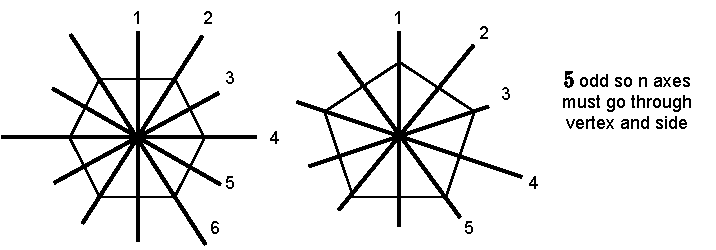
\includegraphics[width=0.65\textwidth]{Figures/AxisChoiceforB-Dihedral.pdf}
    \item $D_n$ is completely determined by its generators and the relations:
    \begin{align}
        a^n&=e\nonumber \\
        b^2&=e \nonumber \\
        ba&=a^{n-1}b \nonumber
    \end{align}
    \item $o(D_n)=2n$ the elements are:
    \begin{align}
        &a,a^2,a^3, ... , a^{n-1},e \nonumber \\
        &b,ab,a^2b, ... , a^{n-1}b \nonumber
    \end{align}\\
    These elements give a closed system...
    \item There is a non-abelian group of every even order $> 4$.
 
    \begin{tabular}{|c|c|c|c|c|c|} \hline
            Order: & 6&8&10&12&14   \\
             Group: &$D_3$ &$D_4$&$D_5$&$D_6$&$D_7$ \\ \hline 
    \end{tabular}
    
    Note $D_7$ corresponds to the symmetries of a "heptagon" $\smiley{}$. Also note that since $o(D_3)=6$ then by Lagrange, if $H < D_3 \ \implies o(H)$ can be $1,\underbrace{2,3}_{\text{primes}}$ or $6$. \steezybreak\\
    Lagrange Cor \#5: groups of prime order are cyclic. \\
    \begin{align}
        \{\underset{1}{e},\underset{3}{a},\underset{3}{a^2},\underset{2}{b},\underset{2}{ab},\underset{2}{a^2 b}\} \nonumber
    \end{align}
    $4$ non-trivial subgroups. \\
    \begin{tabular}{c|cccccc} 
            $D_3$ & $e$ & $a$ & $a^2$& $b$ & $ab$ & $a^2 b$   \\ \hline 
            $e$ & $e$ & $a$ & $a^2$& $b$ & $ab$ & $a^2 b$   \\  
            $a$ & $a$ & $a^2$ & $e$& $ab$ & $a^2 b$ & $b$   \\ 
            $a^2$ & $a^2$ & $e$ & $a$& $a^2 b$ & $b$ & $ab$   \\  
            $b$ & $b$ & $a^2 b$ & $ab$& $e$ & $a^2$ & $a$   \\  
            $ab$ & $ab$ & $b$ & $a^2b$& $a$ & $e$ & $a^2$   \\  
            $a^2 b$ & $a^2 b$ & $ab$ & $b$& $a^2$ & $a$ & $e$   \\  
    \end{tabular}
\end{enumerate}
\steezybreak
\begin{tcolorbox}
    \begin{center}
        $\star\star\star$ \textbf{Read up to this point to Complete Homework 6} $\star\star\star$
    \end{center}
    \end{tcolorbox}
\steezybreak
\section{Cayley's Theorem}
Arthur Cayley (1821-1895) -- set down modern definition of Groups. He was a total G-daddy dog. Used to be a lawyer, Cambridge picked him up to work in Mathematics.

\subsection*{Automorphic bijections as permutations}
Suppose $S$ is a set with $n$ elements. A bijection of $S$ to itself can be viewed as a permutation of the elements of $S$. Recall $S_3=\{\text{bijections on a set of $3$ elements.}\}$\steezybreak\\
Element $\sigma\tau$ in $S_3$ was this bijection:\\
\begin{center}
    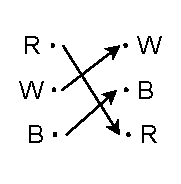
\includegraphics[width=0.3\textwidth]{Figures/Permutations_Cayley_1.pdf} 
\end{center}
So $\sigma \tau$ permutes $RWB \rightarrow WBR$\\
\begin{align}
    S_3= \{\underset{I}{RWB},\underset{\sigma}{RBW},\underset{\tau}{BWR},\underset{\sigma\tau}{WBR},\underset{\tau\sigma}{BRW},\underset{\sigma\tau\sigma}{WRB}\} \nonumber
\end{align}
In general, $S_n= \{\text{Permutations on $n$ elements}\}$ is a group under composition with $o(S_n)=n!$, as we noted before, $S_n$ can alternatively be called $A(S)$ (automorphisms), this name is usually reserved for cases where $S$ has infinite members/elements.
\newpage

\begin{theorem}[Cayley's Theorem] 
Every group $G$ is isomorphic to a subgroup of $A(G)$.
\begin{itemize}
    \item In other words: Every group has the structure of some permutation group.
    \item So permutation groups contain all possible group structure.
\end{itemize}
%(for finite $G$) (idk if that's true, any group can act on itself by left product and this is exactly how we define tau and then psi... I believe this proof holds for any G! (finite or infinite!) although the beginning of part 1's explanation is easier to think of in terms of finite G... but nothing stops you from imagining an infinite cayley table and the "b-row" intuition doesn't stop us from constructing a well-defined mapping \tau_g for each (even infinitely many ) g \in G!
\textit{Proof:} 
\begin{enumerate}
   \item Each row in the Cayley table for $G$ is a permutation of $G$'s elements and each permutation produces a bijection from $G\rightarrow G$.\\%$\blacksquare$ \steezybreak\\
\hrule
%Boy that was quick... how about an example to crystallize the argument above...\steezybreak\\
\textbf{Example:} $b$-row of Cayley table gives $y$ values for the map "L-multiply by $b$"
\begin{align}
    &\tau_b : G\rightarrow G \nonumber \\
    &\tau_b(x)=bx \ \forall \ x \in G \nonumber 
\end{align}
\hrule
Now,
\begin{align}
    \forall \ g\in G, \text{ define } &\tau_g: G\rightarrow G \nonumber \\
    \text{by }&\tau_g(x)=gx \ \forall \ x \in G. \nonumber
\end{align}
\textit{Claim:} $\tau_g$ has an inverse, namely $\tau_{g^{-1}}$\\
\textit{Proof:} $x\in G$
\begin{align}
    (\tau_{g^{-1}} \circ \tau_g)(x)&=\tau_{g^{-1}}(gx)=g^{-1}gx=ex=x \nonumber \\
    (\tau_g \circ \tau_{g^{-1}})(x)&=\tau_{g}(g^{-1}x)=gg^{-1}x=ex=x \nonumber \\
    \therefore (\tau_{g^{-1}} \circ \tau_g) &= I_G \text{ and } (\tau_g \circ \tau_{g^{-1}})= I_G \nonumber \\
    \therefore \tau_g &\text{ has and inverse.} \nonumber \\
    \therefore \tau_g &\text{ is a bijection by Lemma 1.2.3} \nonumber
\end{align}
So $\tau_g \in A(G)$
\item Define $\psi:G\rightarrow A(G)$ by $\psi(g)=\tau_g \ \forall \ g\in G$ \\
$\psi$ is a homomorphism: 
\begin{align}
    &g,g' \in G \nonumber \\
    &\begin{rcases}
    \psi(g\cdot g')=\tau_{gg'}  \\
    \psi(g)\cdot \psi(g')=\tau_{g}\underset{\text{in }A(G)}{\cdot} \tau_{g'} \ \ \ \ 
    \end{rcases}\text{Are these the same?} \nonumber
\end{align}
Take $x\in G$
\begin{align}
    \tau_{gg'}(x)&=gg'x \nonumber \\
    (\tau_g\circ \tau_{g'})(x)&= \tau_g(\tau_{g'}(x))=\tau_g(g'x)=gg'x \nonumber \\
    &\therefore \tau_g\circ\tau_{g'}=\tau_{gg'} \nonumber \\
    &\therefore \psi(gg')=\psi(g)\cdot \psi(g') \nonumber \\
    &\therefore \psi \text{ is a homomorphism.} \nonumber
\end{align}
$\psi$ Injective: Take $g\neq h $ in $G$
\begin{align}
    &\begin{rcases}
    \psi(g)=\tau_g 
    \psi(h)=\tau_h
    \end{rcases} \text{ must show }\tau_g\neq \tau_h \nonumber
\end{align}
Let's see where $e$ gets mapped under $\tau_g$ and $\tau_h$.
\begin{align}
    \tau_g(e)&=ge=g \nonumber \\
    \tau_h(e)&=he=h \nonumber \\
    &\therefore \tau_g(e)\neq \tau_h(e) \nonumber \\
    &\therefore \tau_g \neq \tau_h \nonumber
\end{align}
So $\psi$ is injective. \\
Lastly, we replace $A(G)$ with the image $\psi(G)$ to make $\psi$ surjective
\begin{align}
    &\psi: G\rightarrow \psi(G) \nonumber \\
    &\psi(g)=\tau_g \ \ \ \ \ \ \ \ \text{ (revised defn.)} \nonumber
\end{align}
$\therefore G \ \ \ \overset{\psi}{\approx} \underset{\text{a subgroup of }A(G)}{\psi(G)}. \ \ \ \ \blacksquare$
\end{enumerate}

\end{theorem}

\section{Permutation Groups}
To begin we would like to streamline the notation for permutations... Consider the following diagram\\
\begin{center}
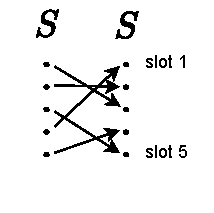
\includegraphics[width=0.25\textwidth]{Figures/Permutation_Notation_ex.pdf}
\end{center}
We will denote this map by $\begin{pmatrix} 1&2&3&4&5\\ 3&2&5&1&4
\end{pmatrix}$ This means 1 goes to 3, 2 goes to 2, 3 goes to 5 and so on.\\
Recall that $S_5$ has order $5!=60$ and now suppose in $S_5$ that 
\begin{align}
    \sigma = \begin{pmatrix}
    1&2&3&4&5\\1&2&4&3&5
    \end{pmatrix} \nonumber \\
    \tau = \begin{pmatrix}
    1&2&3&4&5 \\ 2&4&1&5&3
    \end{pmatrix} \nonumber
\end{align}
We can represent the "product" of these two maps via their composition:
\begin{align}
    \sigma \cdot \tau &= \begin{pmatrix}
    1&2&3&4&5 \\ 1&2&4&3&5
    \end{pmatrix}\begin{pmatrix}
    1&2&3&4&5 \\ 2&4&1&5&3
    \end{pmatrix}\nonumber \\
    &= \begin{pmatrix}
    1&2&3&4&5 \\
    2&4&5&1&3
    \end{pmatrix} \ \ \ \ \ \ \ \ \text{(Thread through maps)} \nonumber
\end{align}


A perceptive reader might notice that this composition is a little different from how we wrote composition before. Normally, we would consider $\sigma \cdot \tau$ to correspond to sigma after tau meaning we should thread through tau then through sigma, however we adopt a notational change that mirrors the original notation of Herstein for composing maps (that is $\sigma \cdot \tau$ should be read as sigma then tau in this section). We use this convention in this section because it makes it easier to read from left to right, threading through consecutive maps.

Now then, with $\sigma$ defined as above, what is the order of $\sigma$ in $S_5$?
\begin{align}
    \sigma^2&=\begin{pmatrix}
    1&2&3&4&5 \\ 1&2&4&3&5
    \end{pmatrix}\begin{pmatrix}
    1&2&3&4&5 \\ 1&2&4&3&5
    \end{pmatrix} = \begin{pmatrix}
    1&2&3&4&5 \\ 1&2&3&4&5
    \end{pmatrix} = e \in S_5 \nonumber \\
    &\therefore \ \ o(\sigma)=2 \nonumber
\end{align}
What is the inverse of $\tau$ defined above?
\begin{align}
    \tau^{-1}= \begin{pmatrix}
    1&2&3&4&5 \\ 3&1&5&2&4
    \end{pmatrix}\nonumber
\end{align}
It is simple to confirm that the above map corresponds to $\tau$'s unique inverse, and in general we can construct inverse map for a map $\tau$ by sending the second row of $\tau$ back to it's first row (notice how $\tau$ sends 1 to 2 and 2 to 4, ... so in order to undo tau we just send 2 to 1, 4 to 2, and so on.)

Let $S$ be a set with $n$ elements and take $\theta \in S_n$, we'll use powers of $\theta$ to define an equivalence relation on $S$. Define the relation $\equiv_{\theta}$ by:
\begin{align}
    a\equiv_{\theta} b \iff \exists i \in \Z \ni b= \theta^i(a) \nonumber
\end{align}

\begin{example}
Consider $S=\{1,2,3,4,5\}$ and
\begin{align}
    \theta = \begin{pmatrix}
    1&2&3&4&5 \\ 5&1&4&3&2
    \end{pmatrix} = (1,5,2)(3,4)\nonumber
\end{align}
Under $\theta$, which elements $b\in S$ are related to $2$?
\begin{align}
    2\equiv_{\theta} b \iff b=\theta^i(2) \ \text{for } i \in \Z \nonumber
\end{align}
Let's have a look at $\theta^i(2)$
\begin{align}
    \theta^0(2)&=2 \nonumber \\
    \theta^1(2)&=1 \nonumber \\
    \theta^2(2)&=5 \nonumber \\
    \theta^3(2)&=2 \nonumber \\
    \text{Negative Powers:} \nonumber \\
    \theta^{-1}(2)&=5 \nonumber \\
    \theta^{-2}(2)&=1 \nonumber \\
    \theta^{-3}(2)&=2 \nonumber
\end{align}
So $b\equiv_{\theta}\theta^i(2)= \{1,2,5\}$, $2, 1$, and $5$ are related to $2$ under $\equiv_{\theta}$
\end{example}
\textbf{Claim:} $\equiv_{\theta}$ is an equivalence relation on $S$. \\
\textit{Proof:}
\begin{enumerate}
    \item \textbf{Reflexive:} $\forall \ a \in S$, $a\equiv_{\theta} a $ because $\theta^0(a)=a$ (applying the theta map 0 times to element a is just element a)
    \item \textbf{Symmetric:} For $a,b \ \in S$ assume that $a\equiv_{\theta} b$, then $\exists \ i \in \Z \ni \ b=\theta^i(a)$, now since $\theta^i \in S_n$, its inverse $[\theta^i]^{-1}\in S_n$, $[\theta^i]^{-1}=\theta^{-i}$. So $\theta^{-i}(b)= \theta^{-i}[\theta^i(a)] = \theta^{-i}\cdot \theta^i(a)=\theta^0(a)=a$, since $a=\theta^{-i}(b)$ and $-i\in \Z$, $b\equiv_{\theta} a$.
    \item \textbf{Transitivity: }Let $a, b, c \ \in S$ and assume $a\equiv_{\theta} b$ and $b\equiv_{\theta} c$,
    \begin{align}
        a&\equiv_{\theta} b \implies \  \exists \ i \in \Z \ni b= \theta^i(a)\nonumber \\
        b&\equiv_{\theta} c \implies \  \exists \ j \in \Z \ni c= \theta^j(b)\nonumber \\
        c&= \theta^j(b)=\theta^j(\theta^i(a))=\theta^{i+j}(a) \nonumber \\
        &\therefore \ \exists \  n=i+j \in \Z \ni c=\theta^n(a) \nonumber \\
        &\therefore \ a \equiv_{\theta} c \nonumber \\
        &\therefore \ \equiv_{\theta} \text{ is transitive.} \ \ \blacksquare \nonumber
    \end{align}
\end{enumerate}
So $\equiv_{\theta}$ partitions $S$ into disjoint equivalence classes. For this relation, these equivalence classes are called ``orbits".

\begin{example}
$\theta= \begin{pmatrix}
1&2&3&4&5 \\ 5&1&4&3&2
\end{pmatrix}$ \\
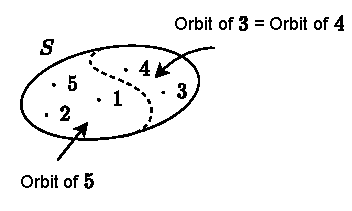
\includegraphics[width=0.6\textwidth]{Figures/Orbits_ex.pdf}\\
A \textit{cycle} is an orbit which is arranged to show the sequence in which  elements are picked up.
\begin{align}
    \text{Orbit of } 2 &= \{1,2,5\} \nonumber \\
    \text{Cycle of } 2 &= (\underset{\longleftarrow}{2^{\rightarrow},1^{\rightarrow},5}) \ \ \ 2 \text{ gets mapped to }1, 1 \text{ gets mapped to } 5, 5 \text{ gets mapped to } 2 \nonumber
\end{align}
The map $\theta$ in this example can be decomposed into a composition of a 3-cycle and a 2-cycle
$(2,1,5)=(1,5,2)=(5,2,1)$ 3-cycle(s) \\
$(3,4)=(4,3)$ 2-cycle.
\end{example}
\begin{definition}[m-cycle]
Let $\theta \in S_n$, $a\in S$\\
\begin{align}
    (a,\theta(a),\theta^2(a), \dots, \theta^m(a))\nonumber
\end{align}
Where $\theta^m(a)=a$ is an \textit{m-cycle} of $S_n$. Here, $m$ denotes the length of the cycle.
\end{definition}
\begin{example}

\begin{align}
\theta &= \begin{pmatrix}
1&2&3&4&5\\5&1&4&3&2
\end{pmatrix}  \nonumber \\
&= (1,5,2)(3,4) \nonumber
\end{align}
So $\theta$ can be written as a product (composition, i.e. ``followed by") of cycles
\end{example}
\begin{example}
\begin{align}
    \theta &= \begin{pmatrix}
1&2&3&4&5&6&7&8 \\
2&7&5&4&6&8&1&3
\end{pmatrix} \nonumber \\
&= (1,2,7)(3,5,6,8)(4) \nonumber
\end{align}
\end{example}
\begin{lemma}
Every permutation has a unique decomposition as a product of disjoint cycles. \\
\textit{Proof:} The sequence of integers in the cycles is determined by the permutation (i.e. a decomposition exists). The sequence can be determined in one way only (it's unique because it's a bijection). The cycles are equivalence classes under the relation $\equiv_{\text{perm}}$ so they are disjoint; their composition (product) is the same bijection as the permutation. $\blacksquare$
\end{lemma}
\begin{example}
Consider the following elements of $S_6$,
\begin{align}
    \theta= \begin{pmatrix}
    1&2&3&4&5&6 \\ 3&5&1&2&4&6
    \end{pmatrix}, \ \ \tau = \begin{pmatrix}
    1&2&3&4&5&6 \\ 2&1&6&5&3&4
    \end{pmatrix} \nonumber
\end{align}
Now let's find the cycle decomposition of $\tau \theta$
\begin{align}
    \theta &= (1,3)(2,5,4)(6)\nonumber \\
    \tau &= (1,2)(3,6,4,5) \nonumber \\
    \tau\theta &= (1,2)(3,6,4,5)(1,3)(2,5,4)(6) \ \ \ \ (\text{Note that }(1,2) \text{ and } (1,3) \text{ are not disjoint, so we must reduce)} \nonumber \\
    &=(1,5)(2,3,6)\centernot{{(4)}} \ \ \ \ \leftarrow \text{ Customary to Eliminate 1-cycles (they go to themselves)} \nonumber
\end{align}
We arrive at the final expression by noting
\begin{align}
    1 \overset{\text{1st}}{\rightarrow} 2 \overset{\text{2nd}}{\rightarrow} 2 \overset{\text{3rd}}{\rightarrow}2 \overset{\text{4th}}{\rightarrow}5 \overset{\text{5th}}{\rightarrow} 5 \nonumber \\
    2 \overset{\text{1st}}{\rightarrow} 1 \overset{\text{2nd}}{\rightarrow} 1 \overset{\text{3rd}}{\rightarrow}3 \overset{\text{4th}}{\rightarrow}3 \overset{\text{5th}}{\rightarrow}3 \nonumber \\
    3 \overset{\text{1st}}{\rightarrow} 3 \overset{\text{2nd}}{\rightarrow} 6 \overset{\text{3rd}}{\rightarrow}6 \overset{\text{4th}}{\rightarrow}6 \overset{\text{5th}}{\rightarrow}6 \nonumber \\
    4 \overset{\text{1st}}{\rightarrow} 4 \overset{\text{2nd}}{\rightarrow} 5 \overset{\text{3rd}}{\rightarrow}5 \overset{\text{4th}}{\rightarrow}4 \overset{\text{5th}}{\rightarrow}4 \nonumber \\
    5 \overset{\text{1st}}{\rightarrow} 5 \overset{\text{2nd}}{\rightarrow} 3 \overset{\text{3rd}}{\rightarrow}1 \overset{\text{4th}}{\rightarrow}1 \overset{\text{5th}}{\rightarrow}1 \nonumber \\
    6 \overset{\text{1st}}{\rightarrow} 6 \overset{\text{2nd}}{\rightarrow} 4 \overset{\text{3rd}}{\rightarrow}4 \overset{\text{4th}}{\rightarrow}2 \overset{\text{5th}}{\rightarrow}2 \nonumber
\end{align}
Where 1st-5th denote the application of cycles 1 through 5 of the non-reduced expression. We can see that the total effect of the non-reduced expression is the composition of disjoint cycles (1,5) and (2,3,6). Since there are only 6 elements to consider, it is often possible to find the unique disjoint decomposition without having to thread through \textit{each and every} element (e.g. we did not need to see where 6 went because it only had one slot it could land in, the 2 slot.)
\end{example}

\begin{example}
\textbf{Problem:} Suppose $\theta = (1,3,9)(2,4,8,5)(6,10,7)\in S_{10}$. Find the order of $\theta \in S_{10}$. \steezybreak\\
We first note that $S_{10}$ has order $10!=3,628,800$, so counting powers might not be the most efficient approach... let's take a brief detour to think about the order of a cycle... \steezybreak\\
\textbf{Aside:} What's the order of an $m$-cycle?
\begin{align}
    (s,t,u,v,w) \nonumber
\end{align}
In this arbitrary 5-cycle, each element is sent one slot to the right, so
\begin{align}
    (s,t,u,v,w)^2 &= (s,t,u,v,w)(s,t,u,v,w)\nonumber \\
    &= (s,u,w,t,v) \nonumber
\end{align}
since $s$ will be taken to the $t$ slot after the first application and $t$ slot gets taken to $u$ slot after the second application; similarly, $u$ gets taken to the $v$ slot after the first application and $v$ slot gets taken to the $w$ slot after the second application. Let's try cubing
\begin{align}
    (s,t,u,v,w)^3&=(s,t,u,v,w)(s,t,u,v,w)(s,t,u,v,w) \nonumber \\
    &= (s,v,t,w,u) \nonumber
\end{align}
So, for $n$ power, cycle shifts each element $n$ spaces
\begin{align}
    (s,t,u,v,w)^5=I=(s)(t)(u)(v)(w)\nonumber
\end{align}
If power is $r$, the resulting cycle sends each element $r$ slots to the right. We conclude that the order of an $m-$cycle is the length of the cycle, $m$. \steezybreak\\
Back to the problem... What's the order of $\theta \in S_{10}$? It should be the smallest $k\in \Z$ so that $\theta^k= I = e \in S_{10}$
\begin{align}
    \theta^k&=[(1,3,9)(2,4,8,5)(6,10,7)]^k \nonumber \\
    &= \underbrace{(1,3,9)^k}_{\text{order }3}\underbrace{(2,4,8,5)^k}_{\text{order }4}\underbrace{(6,10,7)^k}_{\text{order }3} \nonumber
\end{align}
Note, any common multiple of $3$ and $4$ will send each cycle to $I$, $k$ should be the \textit{least} common multiple. So $k=LCM(3,4)=12$.
\end{example}

In general, if $\theta\in S_{n}$ then $o(\theta)= LCM(\text{lengths of disjoint cycles in the decomposition of }\theta)$
\begin{definition}[Transposition]
A \textit{transposition} is a 2-cycle. Consider the cycle $(a_1,a_2)$,
\begin{center}
    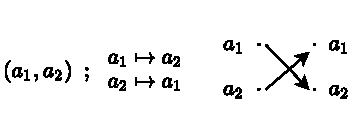
\includegraphics[width=0.4\textwidth]{Figures/transposition_2cycle.pdf}
\end{center}
All other elements are sent to themselves under $(a_1,a_2)$.
\end{definition}

\begin{lemma}
Every permutation can be written as a product of transpositions. \steezybreak\\
\textit{Proof:} By Lemma 2.10.1, it is enough to prove this can be done on cycles, consider an arbitrary $n$-cycle:
\begin{align}
    (a_1, \dots, a_n)=(a_1,a_2)(a_1,a_3)(a_1,a_4)\dots(a_1,a_n). \ \ \blacksquare \nonumber
\end{align}
\end{lemma}
\textbf{NOTE}, the product of transpositions promised by this lemma is \textul{\textbf{NOT}} unique, BUT the number of transpositions involved will either always be \textul{even} or always be \textul{odd} (technical proof omitted, see pg. 79 of Herstein or Theorem 2.1 \href{https://kconrad.math.uconn.edu/blurbs/grouptheory/sign.pdf}{here})
%% Proof that Parity is well-defined (every decomposition into 2-cycles of a permutation \sigma is either always odd or always even )

% Permutation Parity is Well-defined: Given any two representations of $\sigma \in S_n$ as a product of transpositions $\sigma = \tau_1\tau_2 · · · \tau_r = \tau_1' \tau_2' · · · \tau_{r'}' $. Then $r \equiv r' mod 2$ (i.e. $r$ and $r'$ are either both even or both odd). \textit{Proof:} Using the two products of transpositions that equal $\sigma$ above we can express the identity permutation as a product of $r + r'$ transpositions: $(1) = \sigma\sigma^{-1} = \tau_1\tau_2 · · · \tau_r\tau_{r'}'\tau_{r'−1}'· · · \tau_1'.$ (Note $\tau^{−1} = \tau$ for transpositions $\tau$ and inverting a product reverses the order of multiplication.) 

% Claim: A product of transpositions equal to (1) must have an even number of transpositions. This claim forces $r + r '$ above to be even, so $r ≡ r ' mod 2$. To prove the claim, write the identity in $S_n$ as a product of $k$ transpositions: $(1) = (a1b1)(a2b2)· · ·(akbk)$, where $k \geq 1$ and $ai \neq bi$ for all $i$. We want to show $k$ is even and will induct on $k$. The product on the right side of (2.2) can’t have k = 1 since a transposition is not (1). We could have k = 2, which is even. Suppose, by induction, that k ≥ 3 and every product of fewer than k transpositions that equals (1) has an even number of transpositions. Some transposition (aibi) for i 6= 1 has to move a1 (otherwise the overall product on the right side of (2.2) sends a1 to b1, which is not the identity permutation). So a1 must be an ai or bi for i > 1. We can suppose a1 is ai since (aibi) = (biai). The two equations (cd)(ab) = (ab)(cd), (bc)(ab) = (ac)(bc), where different letters are different numbers, show a product of two transpositions where the second one moves a and the first one does not can be rewritten as a product of two transpositions in which the first one moves a and the second one does not. So in (2.2), without changing the number of transpositions we can arrange for a transposition moving a1 other than (a1b1) to appear directly after (a1b1): we can assume a2 = a1. Now consider the cases b2 = b1 and b2 6= b1. Case 1: b2 = b1. The product (a1b1)(a2b2) in (2.2) is (a1b1)(a1b1), which is the identity and can be removed. This turns the right side of (2.2) into a product of k−2 transpositions. By induction, k − 2 is even so k is even. Case 2: b2 6= b1. Check (a1b1)(a2b2) in (2.2), which is (a1b1)(a1b2), can be written as (a1b2)(b1b2) since a1, b1, and b2 are all different. Then (2.2) can be rewritten as (2.3) (1) = (a1b2)(b1b2)(a3b3)· · ·(akbk), where only the first two transpositions have been changed. Now run through the above argument with (2.3) in place of (2.2). It involves the same number k of transpositions, but THE SIGN OF A PERMUTATION 3 there are fewer transpositions in (2.3) that move a1 since we used to have (a1b1) and (a1b2) in the product and now we have (a1b2) and (b1b2).2 Some transposition in (2.3) other than the first term (a1b2) moves a1, so by running through the above argument with (2.3) in place of (2.2) we land in either Case 1, which lets us drop the number of transpositions by 2 and we’re done by induction, or Case 2, which lets us drop the number of transpositions moving a1 by 1 without changing the total number of transpositions. When (1) is a product of transpositions with the leftmost one moving a1, there is always at least one more transposition in the product moving a1 and Case 2 reduces that number by 1. So in finitely many steps we have to land in Case 1 and then we are done. $\blacksquare$




\begin{example}
We illustrate the \textit{non-uniqueness} of the 2-cycle (transpositions) decomposition from the lemma above (Lemma 2.10.2) with a simple example:
\begin{center}
    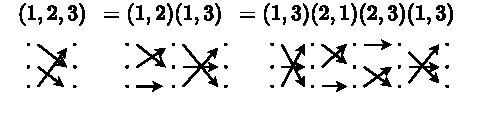
\includegraphics[width=0.75\textwidth]{Figures/non_unique_cycle_trans.pdf}
\end{center}
\end{example}
\begin{definition}[Parity of Permutations]
A permutation $\theta \in S_n$ is \textit{even}, or alternatively \textit{odd}, if it breaks down into an even, or alternatively odd, number of transpositions. The state of $\theta$ as ``even" or ``odd" is called the \textit{parity} of $\theta$.
\end{definition}

\begin{example}
Find the order and parity of $\theta = (1,2,8)(2,4)(3,10,9)(4,7,6)$

\begin{enumerate}
    \item \textbf{Order:} Get disjoint cycles first:
    \begin{align}
        \theta = (1,7,6,4,2,8)(3,10,9)\centernot{(5)}\nonumber
    \end{align}
    So $o(\theta)=LCM(3,6)=6$
    \item \textbf{Parity:} Now let's write the disjoint cycles as a product of 2-cycles:
    \begin{align}
        \theta=(1,7)(1,6)(1,4)(1,2)(1,8)(3,10)(3,9) \nonumber
    \end{align}
    Since we can decompose $\theta$ into $7$ 2-cycles, $\theta$ is an odd permutation.
\end{enumerate}
\end{example}

\begin{example}
What is the parity of $I$, the identity map, which serves as $e\in S_n$?
\begin{align}
    I&=(1)(2)(3)\dots (n) \nonumber \\
    &= (1,2)(2,1)(1,3)(3,1)(1,4)(4,1)\dots (1,n)(n,1) \nonumber
\end{align}
We have $2(n-1)$ transpositions, an even number.\\
$\therefore$ $I$ is an even permutation.
\end{example}

\begin{lemma}
$n\in \Z$, $n\geq 2$. Suppose $A_n$ is the subset of $S_n$ consisting of all even permutations in $S_n$. Then
\begin{align}
    A_n \triangleleft S_n \ \ \text{and} \ \ \  o(A_n)=\frac{n!}{2}\nonumber
\end{align} \\
\noindent \textit{Proof:} We will begin by showing $A_n < S_n$ then we will show $A_n\triangleleft S_n$ and finally we will show $o(A_n)=o(S_n)/2 = n!/2$. \steezybreak\\
$\boxed{A_n < S_n}$ We first note that $I\in A_n$ because it is an even permutation, so we can use Lemma 2.4.2 because $S_n$ is finite ($o(S_n)=n!$). Thus, we need only show that $A_n$ is closed. \steezybreak \\ 
Take $\sigma, \tau \in A_n$, $\sigma$ and $\tau$ are both even permutations.
\begin{align}
    &\sigma \text{ even }\implies \sigma \text{ decomposes into }2k \text{ transpositions for } k\in \Z \nonumber \\
    &\tau \text{ even }\implies \tau \text{ decomposes into }2l \text{ transpositions for } l\in \Z \nonumber \\
    &(\sigma \cdot \tau) = (\text{trans. of }\sigma)(\text{trans. of }\tau)\nonumber \\
    &\therefore \sigma\tau \text{ decomposes into }2k+2l \text{ transpositions} 2(k+l), \ (k+l)\in \Z \nonumber \\
    &\therefore \sigma \tau \text{ is even parity} \nonumber \\
    &\therefore \sigma \tau \in A_n. \ A_n\text{ is closed.} \nonumber \\
    &\therefore A_n < S_n. \nonumber
\end{align}\\
\noindent $\boxed{A_n \triangleleft S_n}$ Now we'll show $A_n$ is the kernel of a homomorphism and $A_n \triangleleft S_n$ will follow by Lemma 2.7.3. \steezybreak\\
Define $\psi : S_n \rightarrow \{-1,1\} \text{ under multiplication}$ (tiny group) its Cayley table looks like this 
\begin{tabular}{r|rr}
$\cdot$ & $1$  & $-1$ \\ \hline
$1$     & $1$  & $-1$ \\
$-1$    & $-1$ & $1$ 
\end{tabular}\\
by the following mapping: $\forall \sigma \in S_n \ \ \psi(\sigma)= \begin{cases}
  \ \ 1 \text{ if even} \\
  -1\text{ if odd}
\end{cases}$\\

\noindent Now, to show $\psi$ is a homomorphism we must show $\psi(\sigma\tau)=\psi(\sigma)\psi(\tau) \ \forall \ \sigma,\tau\in S_n$. \\
\noindent First we note 
\begin{align}
    \psi(\sigma\tau) &= \begin{cases}
      \ \ 1 \text{ if $\sigma\tau$ is even} \\
      -1\text{ if $\sigma\tau$ is odd} 
    \end{cases} \nonumber
\end{align}
Now we consider the cases for parity of $\sigma$ and $\tau$:
\begin{align}
    even-even: \ \ \ \psi(\sigma)\psi(\tau)=1\cdot 1 = 1 \nonumber \\
    odd-odd: \ \ \ \psi(\sigma)\psi(\tau)=-1 \cdot -1 = 1 \nonumber \\
    odd-even: \ \ \ \psi(\sigma)\psi(\tau)=-1\cdot 1 = -1 \nonumber \\
    even-odd: \ \ \ \psi(\sigma)\psi(\tau)=1\cdot -1 - -1 \nonumber
\end{align}
So $\psi$ is a homomorphism. Now we note 
\begin{align}
    \ker\psi &= \{\sigma \in S_n | \psi(\sigma) = 1\} \nonumber \\
    &=\{\text{even permutations}\} \nonumber \\
    &= A_n \nonumber
\end{align}
Since $A_n$ is the kernel of a homomorphism from $S_n$ into another group, $A_n \triangleleft S_n$ (L 2.7.3). \\
\noindent $\boxed{o(A_n)=n!/2}$ To show the final result we recall the First Isomorphism theorem and Lemma 2.6.4. 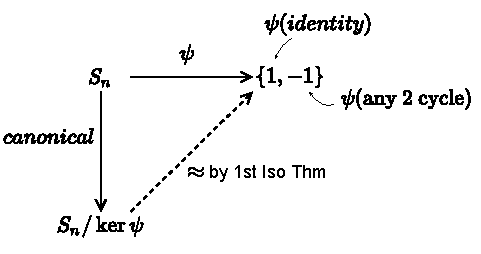
\includegraphics[]{Figures/Lem2-10-3.pdf} \\
Since we can produce pre-images for both -1 and 1, $\psi$ is a surjection and so $S_n/ker\psi$ is isomorphic to $\{-1,1\}$ by the 1st Isomorphism theorem. Therefore $o(S_n/A_n)= 2$. Applying L 2.6.4 we have $o(S_n)/o(A_n)=2 \ \implies \ o(A_n)=n!/2. \ \ \ \blacksquare $
\end{lemma}
\begin{definition}[Alternating Group]
$A_n$ from Lemma 2.10.3 is the \textit{Alternating Group} of degree $n$
\end{definition}

\subsubsection{Importance of Alternating Groups (Example 1)}
Consider the following conjecture, which is the converse of Lagrange's thm: If $m\in \Z^+ \ni \ m | o(G)$, then $G$ has a subgroup of order $m$.  \steezybreak \\
Is this true or false? FALSE!\\ 
$A_4$ shows this is false because $o(A_4) = 4!/2 = 12$ but $A_4$ has no subgroup of order 6!\\
\noindent \textit{Proof:} Suppose $A_4$ has a subgroup of order 6, call it $H<A_4$.\\
$i_{A_4}(H)=2 \ \implies \ H\triangleleft A_4$. Let's figure out the elements of $A_4$, we'll consider elements in $S_4$ to find those in $A_4$.
\begin{itemize}
    \item \textul{4-cycles} $(a,b,c,d)=(a,b)(a,c)(a,d)$, odd $\not\in A_4$
    \item \textul{Product of 2-cycles} $(a,b)(c,d)$  EVEN $\in A_4$
    \item \textul{3-cycles} $(a,b,c) = (a,b)(a,c)$ EVEN $\in A_4$
\end{itemize}
$S=\{1,2,3,4\}$. So $A_4$ has 12 elements, we first look at the order 2 elements
\begin{align}
    (1,3)(2,4) \nonumber \\
    (1,2)(3,4) \nonumber \\
    (1,4)(2,3) \nonumber
\end{align}
Then the order 3 elements
\begin{align}
    (2,3,4) \ \ \ (1,3,4) \ \ \ (1,2,4) \ \ \ (1,2,3)\nonumber \\
    (2,4,3) \ \ \ (1,4,3) \ \ \ (1,4,2) \ \ \ (1,3,2)\nonumber
\end{align}
% \begin{align}
%     (2,3,4) \nonumber \\
%     (2,4,3) \nonumber \\
%     (1,3,4) \nonumber \\
%     (1,4,3) \nonumber \\
%     (1,2,4) \nonumber \\
%     (1,4,2) \nonumber \\
%     (1,2,3) \nonumber \\
%     (1,3,2) \nonumber \\
% \end{align}
Notice how the order 3 elements come in pairs $\alpha, \alpha^2$ e.g. $(1,2,3)= \alpha$ and $(1,3,2) = \alpha^2$ \\
Lastly $A_4$ has a single element of order 1, $(1)(2)(3)(4)$. \steezybreak\\
\noindent Now consider $J=\{(1,2)(3,4), (1,3)(2,4), (1,4)(2,3), e\}$, it can easily be seen that $J$ is closed. (Each product of order 2 elements give third) so $J<A_4$ however $J\not < H$ because $4\not | \ 6$, so $H$ can have at most one element of order 2.

If $H$ has no element of order 2 then $H$ consists of $e$ and 5 order 3 elements, but order 3 elements travel in pairs $\Rightarrow \Leftarrow$. \steezybreak\\

\noindent So $H$ must have exactly 1 order 2 element, call it $\delta$. \\
\noindent Say $\delta = (a,b)(c,d)$. But if we conjugate $\delta$ with the 3-cycle $(a,b,c)$ then
\begin{align}
    &(a,b,c)(a,b)(c,d)(a,b,c)^{-1} \nonumber \\
    =&(a,b,c)(a,b)(c,d)(c,b,a) \nonumber \\
    =&(a,c)(b,d) \in H \ \text{ because } H\triangleleft A_4 \nonumber \\
    &\Rightarrow\Leftarrow \text{ Because $H$ only contains element of order 2 called $\delta$}\nonumber
\end{align}
$\therefore$ Lagrange's converse is false. $\blacksquare$

\subsubsection{Importance of Alternating Groups (Example 2)}
In alternating groups, non-trivial normal subgroups are very sparse. \steezybreak\\
$A_4$ has 8 non-trivial normal sub-groups, only 1 is normal in $A_4$. In fact, for $n\geq 5$ $A_n$ has \textit{none}!

\begin{definition}[Simple Group]
Group $G$ is \textit{simple} if it has no non-trivial normal subgroups. \steezybreak\\
\noindent or:  $G$ simple $\iff$ the only subgroups $\triangleleft G$ are $G$ and $\langle e \rangle$.
\end{definition}

\noindent $\boxed{\textbf{Major Fact:}\ \ \ A_n \text{ is simple for } n\geq 5}$\\
\textit{Several proofs for the above fact exist, many of which are conceptually quite simple, but can get a little lengthy, for this reason we have omitted proof of this fact for the time being... I encourage the reader to explore these proofs on their own.} \steezybreak\\
For a general quadratic polynomial in one variable $ax^2+bx+c=0$ we have all learned that the roots can be solved in radicals (i.e. using only addition, subtraction, multiplication, division, raising to integer powers, and the extraction of nth roots) via the following formula:
\begin{align}
    x = \frac{-b\pm \sqrt{b^2-4ac}}{2a} \nonumber \ \ \ \ \ \ \ \textit{(Babylonian, Hindu, Egyptian and Chinese solutions all existed since BCE)}
\end{align}
What about cubic? Can its roots be solved in radicals?
\begin{align}
    ax^3+bx^2+cx+e=0
\end{align}
$x=??$
\begin{itemize}
    \item $n=3$ cubic: YES! (del Ferro - 1515)
    \item $n=4$ quartic: YES! (Ferrari - 1545)
    \item $n=5$ quintic: NO! $\begin{cases}
      \text{\href{https://en.wikipedia.org/wiki/Niels_Henrik_Abel}{Abel} 1802-1829 (died from TB, in poverty, at 27 \frownie)}\\
      \text{\href{https://en.wikipedia.org/wiki/Evariste_Galois}{Galois} 1811-1832 (died at 21 in a duel)}
    \end{cases}$\\
    NO for $n\geq 5$ $\because$ $A_n$ is simple for $n\geq 5$
\end{itemize}
Abelian groups are named in honor of Abel.
\section{The Class Equation}
\begin{definition}[Conjugacy between Elements]
Let $a\in G$, $G$ a group. \steezybreak\\
Element $b\in G$ is \textit{conjugate} to $a$ $\iff$ $\exists \ g\in G \ni \ gag^{-1}=b$.
\end{definition}

\begin{lemma}
Conjugacy is an equivalence relation. \steezybreak\\
\noindent \textit{Proof:} 
\begin{enumerate}[label=\roman*)]
    \item \textit{Reflexivity:} $a$ is conjugate to itself because $a = eae^{-1}$
    \item \textit{Symmetry:} \begin{align}
        b \textit{ conj. to } a &\implies \exists \ g\in G \ni gag^{-1}=b \nonumber \\
        &\implies ag^{-1}=g^{-1}b \nonumber \\
        &\implies a= g^{-1}bg \nonumber \\
        &\implies a= g^{-1}b(g^{-1})^{-1} \nonumber \\
        \therefore \ a \text{ conj. to } b & \nonumber
    \end{align}
    \item \textit{Transitivity:} Assume \begin{align}
        a \text{ conj. to } b \implies \exists \ g \in G \ni \ gbg^{-1}=a \nonumber \\
        b \text{ conj. to } c \implies \exists \ h \in G \ni \ hch^{-1}=b \nonumber \\
        a = g(hch^{-1})g^{-1} = (gh)c(\underset{\in G}{gh})^{-1} \nonumber \\
        \therefore \ a \text{ conj. to } c. \ \ \ \blacksquare \nonumber
    \end{align}
\end{enumerate}
\end{lemma}
\begin{definition}[Conjugate Class]
The equivalence class of $a\in G$ under conjugacy is the \textit{conjugate class} of $a\in G$ denoted $C(a)$
\begin{align}
    C(a)= \{x \in G | x \text{ is conjugate to } a\}
\end{align}
\end{definition}
For a finite group $G$, we can describe $o(G)$ in terms of the conjugate classes. \steezybreak\\
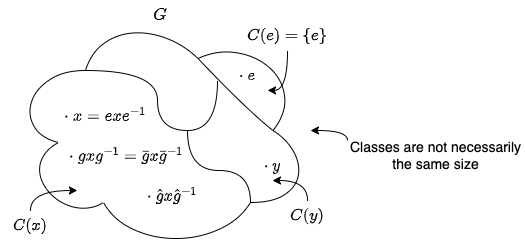
\includegraphics[width=0.95\textwidth]{Figures/Conjugacy_Partition.png}
\begin{align}
    o(G) = \sum_{\substack{\text{one elt. }\\a \text{ from} \\ \text{each conj. class}}}(\text{\# of elts in }C(a)) \nonumber
\end{align}
Recall: If $a\in G$, $N(a)=$normalizer of $a = \{g\in G | ga=ag\}$
\begin{align}
    \forall \ a \in G, N(a)<G \nonumber \\
    N(e) = G \nonumber
\end{align}
If $G$ is abelian then $N(g) = G \ \forall \ g\in G$.
\newpage
\begin{theorem}
If $G$ is a finite group, the number of elements in the class of $a$ ($C(a)$) is the index for the normalizer of that element, $N(a)$. That is,
\begin{align}
    \text{\# of elements in }C(a) \overset{\star}{=} i_G(N(a))= \frac{o(G)}{o(N(a))} \nonumber
\end{align}
Proving $\star$ will give us \textit{the class equation}:
\begin{align}
    o(G) = \sum_{\substack{\text{one  '}a'  \\\text{from each} \\ \text{conj. class}}}\frac{o(G)}{o(N(a))} \ .\nonumber
\end{align}
\textit{Proof:} The number of elements in $C(a)$ is the number of \textit{distinct} conjugates of $a\in G$. (list of $gag^-1 \ \forall \ g\in G$, toss out duplicates, then count).
\begin{align}
    i(N(a))= \text{ the number of left cosets of }N(a) \text{ in }G
\end{align}
We must show the number of distinct conjugates is the same as the number of left cosets of $N(a)$. \steezybreak\\
Plan: set up a mapping (as simply as possible), then try to show it's a bijection. \steezybreak\\
Define $\sigma:C(a)\rightarrow \{\text{left cosets of }N(a)\}$ by 
\begin{align}
    \sigma(gag^{-1})=gN(a)
\end{align}
is $\sigma$ well-defined? Take $x\in C(x)$, it's possible that $x$ might be expressed in more than one way
\begin{center}
    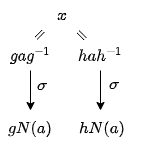
\includegraphics[width=0.19\textwidth]{Figures/sigma_well_def.png}
\end{center}%e.g. $x=gag^{-1}$ and $x=hah^{-1}$, so check that $gN(a)=hN(a)$ 
To be well-defined, $\sigma$ must send each element from the source set to one and only one element in the target set. While $\sigma$ does have somewhere to send every element (since every element in $C(a)$ can be written $gag^{-1}$ for some $g\in G$), we must ensure that when a given element $x$ can be expressed in more than one way, that it always maps to the same place, i.e. we must check that $gN(a)=hN(a)$.
\begin{align}
    gag^{-1} = hah^{-1} &\implies gag^{-1}h=ha \nonumber \\
    &\implies ag^{-1}h=g^{-1}ha \nonumber \\
    &\implies g^{-1}h \text{ commutes with } a \nonumber \\
    &\implies g^{-1}h \in N(a) \nonumber \\
    &\overset{\text{L mult. by }g}{\implies} h\in gN(a) \nonumber \\
    &\text{Now, }\underset{h\in}{gN(a)} \cap \underset{h\in}{hN(a)} \not = \emptyset \nonumber\\
    &\implies gN(a) = hN(a)
\end{align}
So $\sigma$ is well-defined. \\
\noindent \textit{$\sigma$ is surjective:} Take $yN(a) \in \text{codomain}$\\
$\sigma(yay^{-1})=yN(a)$, so $yay^{-1}$ serves as a preimage for $yN(a)$ \steezybreak\\
\noindent \textit{$\sigma$ is injective:} We want to show that this can't happen \\
\begin{center}
    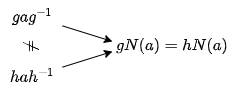
\includegraphics[width=0.4\textwidth]{Figures/noninjective.png}
\end{center}
typically to show injectivity we assume $x\not = y$ and show it follows that $\sigma(x)\not = \sigma(y)$, in this case we will prove injectivity by contraposition so we will show $\sigma(x)=\sigma(y)$ implies $x=y$, or more specifically we will assume $gN(a)=hN(a)$ and we will show this forces $gag^{-1}=hah^{-1}$
\begin{align}
    \text{Assume }gN(a)=&hN(a) \nonumber \\
    g\in hN(a) &\implies \ \exists \ n\in N(a) \ni g = hn \nonumber \\
    gag^{-1}=(hn)a(hn)^{-1}&= h\underline{na}n^{-1}h^{-1} \nonumber \\
    &= hann^{-1}h^{-1} \nonumber \\
    &=hah^{-1} \nonumber
\end{align}
 $\therefore \ \sigma$ is a bijection $\implies$ \# of elements in domain $=$ \# elements in codomain. So $o(C(a))=i_G(N(a))$. $\blacksquare$
\end{theorem}
\subsection*{Applications of the Class Equation}
\subsubsection*{Application \# 1}
\begin{theorem}
$G$ group. If $o(G)$ is a power of a prime, then the center of $G$ is bigger than just $\{e\}$.
\begin{align}
    o(G) = p^n (p \text{ prime}) \implies \text{center of }G \text{ is non-trivial} \nonumber
\end{align}
\textit{Proof:} 
\begin{align}
    a\in Z(G) &\iff ag=ga \ \forall \ g \in G \nonumber \\
    &\iff N(a)=G \nonumber \\
    &\iff i_G(N(a))=1 = \frac{o(G)}{o(N(a))}=\frac{o(G)}{o(G)} \nonumber \\
    &\underset{Thm \ 2.11.1}{\iff} \text{\# of elts. in }C(a) = 1 \nonumber \\
    &\iff C(a) = \{a\}  \ \ \ \ \ (\text{note }gag^{-1}=agg^{-1} = a \text{ since }a\in Z(G)) \nonumber
\end{align}
\begin{center}
    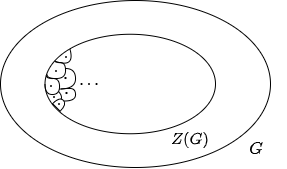
\includegraphics[width=0.45\textwidth]{Figures/shattered_center.png}
\end{center}
The partition of $G$ into equivalence classes shatters $Z(G)$ into one-point classes. Classes outside the center contain $>1$ element (notice the chain of iff statements above implies that having exactly one element in $C(a)$ is equivalent to $a\in Z(G)$).
\begin{align}
    \text{Assume } o(G)=p^n \nonumber \\
    \text{Say }o(Z(G))=\beta \ \ \ e\in Z(G) \implies \beta \geq 1 \nonumber
\end{align}
Use class equation:
\begin{align}
    o(G)= \sum_{\substack{\text{one  '}a'  \\\text{from each} \\ \text{conj. class}}} \frac{o(G)}{o(N(a))} = \beta + \sum_{\substack{\text{one $a$ } \\\text{from each }\\ \text{class outside} \\ Z(G)}} \frac{o(G)}{o(N(a))}\nonumber
\end{align}
Notice for the sum after the second equality, $N(a)<G$ but $N(a)\not = G$ because each $a$ in this sum is \textit{outside} $Z(G)$ so these $a$'s don't commute with everything. \steezybreak\\
Lagrange says $o(N(a))|o(G)=p^n$, so $o(N(a))$ is one of these: $1,p,p^2, \dots , p^{n-1}$. Say it's $p^{K_a}$, $K_a<n$ since $N(a)\not = G$, we have
\begin{align}
    p^n = \beta + \sum_{\substack{\text{one }a \\ \text{for each} \\ \text{conj. class} \\ \text{outside }Z(G)}} \frac{p^n}{p^{K_a}} = \beta + \sum p^{n-K_a}\nonumber
\end{align}
Solve for $\beta$:
\begin{align}
    \beta = p^n - \sum p^{n-K_a} \nonumber
\end{align}
Now, $p$ divides the right side so $p|\beta$. \steezybreak\\
If $\beta = 1$ then $p|1$, since no prime divides 1 $\Rightarrow\Leftarrow$, so $\beta \not = 1$. \\ So $\beta > 1$ and $G$ has non-trivial center. $\blacksquare$
\end{theorem}

\subsubsection*{Application \# 2 (Corollary to Thm 2.11.2)}
In the proof below we use a new symbol $A\subsetneqq B$ to indicate that $A$ is a strict subset of $B$, this symbol is equivalent to $A \subset B$ \textit{and} $B \not \subset A$
\begin{corollary}
A group of order $p^2$ ($p$ prime) is abelian. \steezybreak\\
\noindent \textit{Proof:} Suppose $o(G)=p^2$, we will show $Z(G)=G$.\steezybreak\\
Now, $Z(G)<G \ \ \implies o(Z(G)) = 1, \ p, \ \text{ or} \underbrace{p^2}_{\text{we want this}}$. \steezybreak\\
By Thm 2.11.2, $Z(G)$ is bigger than $\{e\}$ so order of $Z(G)$ is not $1$. What if $o(Z(G))= p$?
\begin{center}
    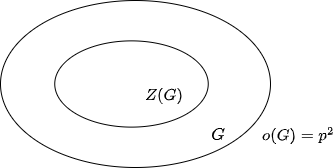
\includegraphics[width=0.5\textwidth]{Figures/Center_of_G.png}
\end{center}
Then $\exists \ a \in G \ni \ a \not\in Z(G)$ \steezybreak\\
Consider $N(a)$: 
\begin{align}
    \underset{a\not \in }{Z(G)} \subsetneqq &\underset{a\in}{N(a)}, \text{ so order of }N(a)>p \nonumber \\ 
    \text{Now, since }N(a) < G, \ \ o(N(a))>p &\implies o(N(a))=p^2 \nonumber \\
    &\implies N(a) = G \nonumber \\
    &\implies a \text{ commutes with everything!} \Rightarrow\Leftarrow
\end{align}
($\Rightarrow\Leftarrow$ because $a\not\in Z(G)$) \steezybreak\\
This contradiction gives that $o(Z(G))\not = p$ \steezybreak\\
So $o(Z(G))$ must be $p^2$, thus $Z(G)=G$ \steezybreak\\
$\therefore$ $G$ is abelian. $\blacksquare$
\end{corollary}

How much information do you get about a group from its order?
\subsection*{Fact Collection w.r.t. $o(G)=p, \ p^2, \ p^n, ...$ ($p$ prime): }
\subsubsection*{$o(G)=p$}
\begin{center}
    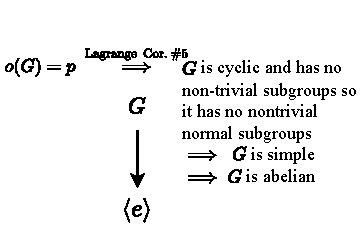
\includegraphics[width=0.495\textwidth]{Figures/prime_order_lattice.pdf}
    \begin{align}
        \Z_7 = \{0,1,2,3,4,5,6\} \text{ under } \ +\mod 7\nonumber
    \end{align}
\end{center}
\subsubsection*{$o(G)=p^2$}
\begin{align}
        o(G)=p^2 \ \implies G \text{ abelian} \ \implies \text{All subgroups of }G \text{ are normal in }G. \nonumber 
\end{align}
\begin{center}
    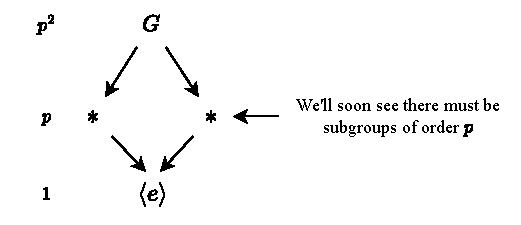
\includegraphics[width=0.7\textwidth]{Figures/prime_squared_order_lattice.pdf}
\end{center}
\subsubsection*{$o(G)=p^n$}
\begin{center}
    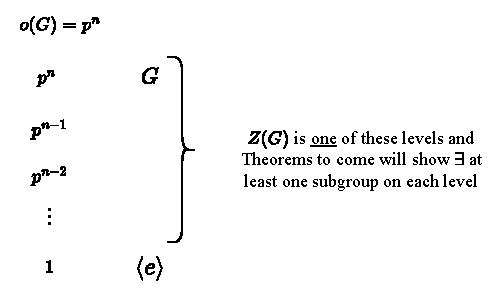
\includegraphics[width=0.68\textwidth]{Figures/prime_power_order_lattice.pdf}
\end{center}
\begin{tcolorbox}
    \begin{center}
        $\star\star\star$ \textbf{Read up to this point to Complete Homework 7} $\star\star\star$
    \end{center}
\end{tcolorbox}

\section{\texorpdfstring{The Sylow Theorems ( $G$ finite )}{The Sylow Theorems ( G finite )}}
Lagrange's theorem tells us that the order of a subgroup of a finite group is a divisor of the order of that group. The converse, however, is false. There are very few theorems which assert the existence of subgroups of prescribed order in arbitrary finite groups. The most basic, and widely used, is a classic theorem due to the Norwegian mathematician Peter Sylow (1832-1918).
In this section we will present this classic result. \\

\noindent Before beginning the proof of Sylow's first theorem, we will take a slight detour to a number-theoretic and combinatorial argument that will be useful in our proof: \\
The number of ways of picking a subset of $k$ elements from a set of $n$ elements can easily be shown to be 
\begin{equation}
    {n \choose k} = {\frac{n!}{k!(n-k)!}} \nonumber
\end{equation}

If $n=p^\alpha m$ where $p$ is a prime number, and if $p^r|m$ but $p^{r+1}\not | \ m$, consider
\begin{align}
    {p^\alpha m \choose p^\alpha} &= \frac{(p^\alpha m)!}{(p^\alpha)!(p^\alpha m - p^\alpha)!} \nonumber \\
    &= \frac{p^\alpha m (p^\alpha m -1)(p^\alpha m - 2)\dots(p^\alpha m - p^\alpha + 1)\overbrace{(p^\alpha m - p^\alpha)(p^\alpha m -p^\alpha -1)\dots(p^\alpha m - p^\alpha m + 1)}^{(p^\alpha m -p^\alpha)!}}{(p^\alpha)!(p^\alpha m -p^\alpha)!} \nonumber \\
    &= \frac{p^\alpha m (p^\alpha m -1)(p^\alpha m - 2)\dots(p^\alpha m - p^\alpha + 1)}{(p^\alpha)!} \nonumber \\
    &= \frac{p^\alpha m (p^\alpha m -1) \dots (p^\alpha m - i) \dots (p^\alpha m - p^\alpha +1)}{p^\alpha (p^\alpha -1) \dots (p^\alpha - i) \dots (p^\alpha - p^\alpha +1)} \nonumber \\
    &= m\cdot \frac{p^\alpha (p^\alpha m -1) \dots (p^\alpha m - i) \dots (p^\alpha m - p^\alpha +1)}{p^\alpha (p^\alpha -1) \dots (p^\alpha - i) \dots (p^\alpha - p^\alpha +1)} \nonumber \\ 
    &= m\cdot \frac{ (p^\alpha m -1) \dots (p^\alpha m - i) \dots (p^\alpha m - p^\alpha +1)}{ (p^\alpha -1) \dots (p^\alpha - i) \dots (p^\alpha - p^\alpha +1)}
\end{align}
The question is, What power of $p$ divides ${p^\alpha m \choose p^\alpha}$? We will show that $p^r | {p^\alpha m \choose p^\alpha}$ but $p^{r+1} \not | {p^\alpha m \choose p^\alpha}$. \\
\textit{Proof:} Let $m\geq 1$, and $0<i<p^\alpha$, with $m,i,p,\alpha,\beta \in \Z$. \steezybreak\\ In order to prove our claim, we will begin by showing that the fraction on the right of equation (2.7) cannot provide any factors of $p$ since each numerator term that could provide a factor of $p$ will cancel with a corresponding term in the numerator. That is, we will begin by proving the following claim. \steezybreak\\
\textit{Claim 1: } $p^\beta | p^\alpha m - i \ \iff p^\beta | p^\alpha - i$  for $0<i<p^\alpha$\steezybreak\\
\textit{Proof of Claim 1:}\steezybreak\\
\textbf{$\Leftarrow$ :} Suppose $p^\beta | p^\alpha -i $
\begin{align}
  &\implies \exists \ h \in \Z \ni hp^\beta = p^\alpha - i \ \ \ \ \ (\text{Note, }i<p^\alpha \implies h > 0)\nonumber \\
  &\implies i = p^\alpha - hp^\beta \nonumber \\
  &\implies p^\alpha m -i = p^\alpha m - p^\alpha + hp^\beta \nonumber \\
  &\implies p^\alpha m -i = p^\beta (p^{\alpha-\beta}m-p^{\alpha-\beta}+h) \nonumber
\end{align}
\indent \textit{claim: } $\beta < \alpha$, otherwise $i=p^\alpha - \underbrace{h}_{>0}p^\beta \leq 0, \text{ but } i>0 \Rightarrow \Leftarrow \ \text{So } \beta < \alpha$
\begin{align}
    &\implies p^{\alpha -\beta} \in \Z \nonumber \\
    &\implies (p^{\alpha-\beta}m-p^{\alpha-\beta}+h) \in \Z \nonumber \\
    &\implies p^\beta | p^\alpha m -i \nonumber
\end{align}

\textbf{$\Rightarrow$:} Suppose $p^\beta | p^\alpha m -i$
\begin{align}
    &\implies \exists \ g \in \Z \ni gp^\beta = p^\alpha m -i \nonumber \\
    &\implies i = p^\alpha m -gp^\beta \nonumber \\
    &\implies p^\alpha - i = p^\alpha - p^\alpha m + gp^\beta \nonumber \\
    & \ \ \ \ \ \ \ \ \ \ \ \ \ \ \ \ \ \ \ \ = p^\beta (p^{\alpha-\beta} -p^{\alpha-\beta}m + g) \nonumber
\end{align}
\indent \textit{claim: } $\beta < \alpha$, otherwise 
\begin{align}
    i &= p^\alpha m - gp^\beta \nonumber \\
    \implies p^\alpha -i &= p^\alpha - p^\alpha m + gp^\beta \nonumber \\
    &= p^\alpha \underbrace{((1-m)+gp^{\overbrace{\scriptstyle\beta-\alpha}^{>0}})}_{\in \Z} \nonumber \\
    &\implies p^\alpha | p^\alpha - i \ \ \Rightarrow\Leftarrow \nonumber 
\end{align}
So $\beta < \alpha \ \ \implies (p^{\alpha-\beta}-p^{\alpha-\beta}m+g)\in \Z$ $ \ \ \ \implies \ \ p^\beta | p^\alpha - i$. This completes the proof of claim 1. \steezybreak\\
With Claim 1 established we can now see that if there were some numerator term $p^\alpha m - i$ for $0<i<p^\alpha$ that has a power of $p$ as a factor then there is \textit{necessarily} a corresponding term in the denominator ($p^\alpha -i$) which cancels this power of $p$. This means if any power of $p$ divides ${p^\alpha m \choose p^\alpha}$ it must do so by dividing the $m$ out front in equation (2.7). Thus
\begin{align}
    p^r | {p^\alpha m \choose p^\alpha} \text{ but } p^{r+1} \not | {p^\alpha m \choose p^\alpha} \ \ \ \ \ \ \blacksquare \nonumber 
\end{align}
%Looking at this number how we have it written out in the last line, we can see that except for the term $m$ in the numerator, the power of $p$ dividing $(p^\alpha m -i)$ is the same as that dividing $p^\alpha$

\begin{theorem}[Sylow's Theorem (Sylow \#1)]
$G$ finite. If $p$ is prime and $p^\alpha|o(G)$ then $G$ has a subgroup of order $p^\alpha$ \steezybreak\\
\textit{Proof:}
Let $\mathcal{M}$ be the set of all subsets of $G$ which have $p^\alpha$ elements. Since $p^\alpha | o(G)$, $o(G)$ can be written $o(G)=p^\alpha m$ for some $m\in \Z \ni m \geq 1$. Thus $\mathcal{M}$ has ${p^\alpha m \choose p^\alpha}$ elements. Given $M_1 , M_2 \in \mathcal{M}$ ($M_1$ is a subset of $G$ having $p^\alpha$ elements, and likewise so is $M_2$ ) define $M_1 \sim M_2$ if there exists an element $g \in G$ such that $M_1 = M_2g$. It is immediate to verify that this defines an equivalence relation on $\mathcal{M}$.
\begin{enumerate}[label=\roman*)]
    \item Reflexivity: $M_1=M_1e$, $e\in G$
    \item Symmetry: Let $M_1\sim M_2 $
    \begin{align}
        &\implies \exists \ g\in G \ni M_1=M_2g, \nonumber \\
        &\implies M_1g^{-1} = M_2gg^{-1}=M_2 \nonumber \\
        G \text{ group } &\implies \ g^{-1}\in G \nonumber \\
        &\implies M_2\sim M_1 \nonumber 
    \end{align}
    \item Transitivity: Let $M_1\sim M_2$ and $M_2\sim M_3$
    \begin{align}
        M_1\sim M_2 &\implies \exists \ g \in G \ni M_1= M_2g \nonumber \\
        M_2\sim M_3 &\implies \exists \ h \in G \ni M_2= M_3h \nonumber \\
        &\implies M_1 = (M_3h)g = M_3(hg) \ \  hg\in G \text{ by closure.} \nonumber
    \end{align}
\end{enumerate}


We claim that there is at least one equivalence class of elements in $\mathcal{M}$ such that the number of elements in this class is not a multiple of $p^{r+1}$, for if $p^{r+1}$ is a divisor of the size of each equivalence class, then $p^{r+1}$ would be a divisor of the number of elements in $\mathcal{M}$ (remember observation 4 about division and that an equivalence relation on a set partitions the set). Since $\mathcal{M}$ has ${p^\alpha m \choose p^\alpha}$ elements and $p^{r+1} \not | {p^\alpha m \choose p^\alpha}$ this cannot be the case. Let ${M_1, \dots , M_n}$ be such an equivalence class in $\mathcal{M}$ where $p^{r+1}\not | \ n $. By our very definition of equivalence in $\mathcal{M}$, if $g \in G$, for each $i = 1, \dots , n$, $M_ig = M_j$ for some $j, 1 \leq j \leq n$. We let $H = \{g \in G | M_1g = M_1 \}$. Clearly $H$ is a subgroup of $G$ by Lemma 2.4.2, for if $a, b \in H$, then $M_1a = M_1 $ and $ M_1 b = M_1$ therefore $M_1ab = (M_1a)b = M_1b =M_1$. We would like to show $o(H)=p^\alpha$. We first claim that $n\cdot o(H) =o(G)$. \steezybreak\\
\textit{Proof of Claim:}
We will prove that $no(H)=o(G)$ by first showing that there is a bijection from $\{Ha | a \in G\}$ to $\{M_1,\dots M_n\}$. \steezybreak\\
Let $C= \{Ha|a\in G\}$ be the set of right cosets of $H$. Then,
\begin{align}
    |C| = \frac{o(G)}{o(H)} 
\end{align}
Note that
\begin{align}
    Ha=Hb \iff ab^{-1} \in H \iff M_1 ab^{-1} = M_1 \iff M_1a=M_1b .\nonumber
\end{align}
Therefore the function $\sigma:C\rightarrow \mathcal{M}$ given by $\sigma(Ha)=M_1 a$ is well-defined and injective. Since $M_1aa^{-1}=M_1$, we have $M_1a\sim M_1$ and thus $\sigma(C) \subset \{M_1,M_2,\dots M_n\}$. On the other hand, each $M_i$ has the form $M_1a_i$ because $M_i \sim M_1$. So, $M_i = \sigma(Ha_i)$ and thus $\{M_1, \dots, M_n\} \subset \sigma(C)$. This shows that $\sigma(C)= \{M_1, \dots , M_n\}$. So $\sigma$ is a one-to-one correspondence (a bijection), we conclude that
\begin{align}
    |C|=|\{M_1,\dots M_n\}|
\end{align}
Equations (2.8) and (2.9) imply $|C|o(H)=n\cdot o(H)=o(G)$. This completes the proof of the claim.

Now $no(H) = o(G) = p^\alpha m$; since $p^{r+1}\not | n$ and $p^{r+\alpha}|p^{\alpha}m = no(H)$, it must follow that $p^\alpha | o(H)$, and so $o(H)\geq p^\alpha$. However, if $m_1 \in M_1$ , then for all $h\in H, m_1h \in M_1$. Thus $M_1$ has at least $o(H)$ distinct elements. However, $M_1$ was a subset of $G$ containing $p^\alpha$ elements. Thus $p^\alpha \geq o(H)$. Combined with $o(H) \geq p^\alpha$ we have that $o(H) = p^\alpha$. \textit{But then we have exhibited a subgroup of $G$ having exactly $p^\alpha$ elements, namely $H$.} This proves the theorem; it actually has done more -- it has constructed the required subgroup before our very eyes! $\blacksquare$

\end{theorem}

\begin{example}
Consider $A_4$ whose order is $o(A_4)= \frac{4!}{2} = 12 =2^2\cdot 3$ \\ 
\noindent Sylow \#1 $\implies$ $A_4$ has subgroups of order $2,2^2$ and $3$ \steezybreak\\
\noindent Sylow \#1 tells us nothing about $6$ because $6$ is not a prime power.
\end{example}

\begin{definition}[p-Sylow Subgroup]
If $H<G$ and $o(H)=p^m$ where $p^m|o(G)$ but $p^{m+1}\not | o(G)$, the $H$ is a \textit{p-Sylow subgroup} of $G$.
\end{definition}

\begin{example}
Given $G$ with $o(G)=72=8\cdot 9=2^3\cdot 3^2$, Sylow \#1 says $G$ has subgroups of order $2,2^2,2^3,3,3^2$. The order $8$ subgroups are $2-$Sylow subgroups and the order $9$ subgroups are $3-$Sylow subgroups.
\end{example}
\begin{example}
Let $o(G)=8=2^3$, the $2-$Sylow subgroup is the trivial group $G$.
\end{example}

To save on time the next two theorems will be provided without proof as we are currently more interested in the insights that can be gained from the results themselves. (Jack, get some proofs for these!)

\begin{theorem}[Sylow \#2] 
For a given prime $p$, the $p-$Sylow subgroups are conjugate to each other.
\end{theorem}
Sylow \#2 says that if you know one $p-$Sylow subgroup $H$, you can find the rest of the $p-$Sylow subgroups by conjugating $H$.\\
\begin{center}
    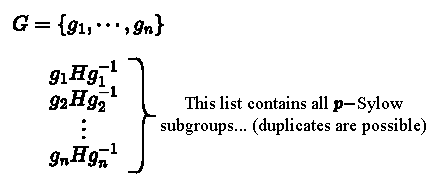
\includegraphics[width=0.5\textwidth]{Figures/Sylow2_conjugates.pdf} 
\end{center}
\begin{theorem}[Sylow \#3]
Suppose $p^m|o(G)$ but $p^{m+1}\not | o(G)$. The number of $p-$Sylow subgroups in $G$:
\begin{enumerate}
    \item divides $\frac{o(G)}{p^m}$ (the index of the $p-$Sylow subgroup) \steezybreak\\
    \noindent AND
    \item is congruent to $1\mod p$ \ \ \ (i.e. is $1+kp$ for some $k\in \Z$)
\end{enumerate}
\end{theorem}
\begin{example}
Let $o(G)=12=2^2\cdot 3$ \steezybreak\\
Sylow \#1 guarantees that $G$ has $2-$Sylow subgroup(s) of order $4$, $3-$Sylow subgroup(s) of order 3, and at least one subgroup of order $2$. \steezybreak\\
How many $2-$Sylow subgroups are there? \steezybreak\\
Sylow \#3 says the number of $2-$Sylow subgroups must divide the index of $2-$Sylow (12/4 = 3) and must be congruent to 1 mod 2 so there are either 1 or 3 $2-$Sylow subgroups. \steezybreak\\
($A_4$ has one subgroup of order 4; $D_6$ has 3 subgroups of order 4) \steezybreak\\
How many $3-$Sylow subgroups? Well the first part of Sylow \#3 tells us the number of $3-$Sylow subgroups divide $\frac{12}{3}=4$ making 1, 2, and 4 candidates, the second part of Sylow \#3 says the number must be $\equiv 1\mod 3$ which eliminates $2$ as a candidate, so there must be 1 or 4 $3-$Sylow subgroups. \steezybreak\\
($A_4$ has 4 ; $D_6$ has 1)
\newpage
\end{example}

\subsection*{Applications of Sylow Theorems}
\begin{enumerate}
    \item Prove no group of order $50$ is simple. \steezybreak\\
    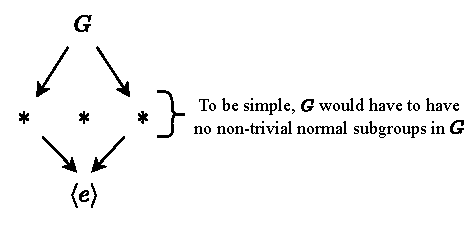
\includegraphics[width=0.575\textwidth]{Figures/order50_no_normal.pdf} \steezybreak\\
    \textit{Proof:} $G$ group with order $o(G)=50=2\cdot 5^2$, $G$ has subgroups of order $2, 5, 25$. Consider one of the subgroups of order $25$, call it $H$
    \begin{align}
        &i_G(H)=2 \ \ \overset{Cor \ 2.6.2}{\Longrightarrow} \ \  H\triangleleft G \nonumber \\
        &\therefore G \text{ is not simple.} \ \ \blacksquare \nonumber
    \end{align}
    \item Any two groups of order $15$ are isomorphic. \steezybreak\\
    \textit{Proof: } Suppose $G$ is a group and $o(G)=15=3\cdot 5$\\
    Sylow \#1 $\implies$ $\exists$ in $G$ at least one subgroup of order $3$ and one of order $5$.\\
    Sylow \#3 $\implies$ \# of $5-$Sylow subgroups must divide $\frac{15}{5}=3$ (so $1$ or $3$) AND must be $\equiv 1\mod 5$ $\implies$ there is exactly 1 subgroup of order $5$, call it $H$\\
    Sylow \#3 $\implies$ \# of $3-$Sylow subgroups must divide $\frac{15}{3}=5$ (so $1$ or $5$) AND must be $\equiv 1\mod 3$ $\implies$ $G$ has exactly one subgroup of order $3$, call it $K$.\\
    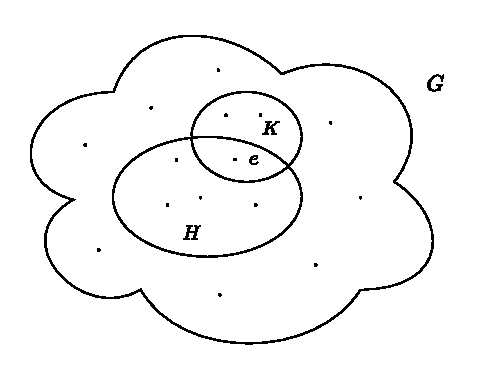
\includegraphics[width=0.5\textwidth]{Figures/order15_subgroups.pdf}\\
    \begin{align}
        &H\cap K < H \text{ and } H\cap K < K \nonumber \\
        &\text{Take }x\in G, x\not\in H\cup K \nonumber \\
        &\text{Order of }x \text{ can be }1, 3, 5,\text{ or }15 \nonumber\\
        &x\text{ is not } e \text{ so order }\neq 1 \nonumber \\
        &\text{If }o(x)=3, \text{ then } \langle x \rangle = K \nonumber \\
        &\Rightarrow\Leftarrow x \not \in K \nonumber \\
        &\text{If }o(x)=5, \text{ then } \langle x\rangle = H \nonumber \\
        &\Rightarrow\Leftarrow x\not \in H \nonumber
    \end{align}
    So the order of $x$ must be $15$. \steezybreak\\
    So $\langle x \rangle = G$. \steezybreak\\
    $\therefore \ \ G$ is cyclic. \\
    So any group of order $15$ is cyclic. If $o(G)=o(\bar{G})=15$ then $G$ and $\bar{G}$ are isomorphic because any 2 cyclic groups of the same order are isomorphic (important fact right before the 1st Isomorphism Theorem). $\ \ \ \ \blacksquare$
    \item Any group of order 20,449 is abelian. \steezybreak\\
    \noindent \textit{Proof:} Let $o(G)=20,449=11^2\cdot 13^2$ \steezybreak\\
    Sylow \#3 $\implies$ \# of 11-Sylow subgroup(s) divides $\frac{o(G)}{11^2}=13^2$ : \# is $1$, $13$, or $13^2$. Also, \# $\equiv 1 \mod 11$, remove 13 because $13\equiv 2\mod 11$ and $13^2\equiv 4\mod 11$. So $G$ has exactly $1$ 11-Sylow subgroup, call it $H$. \steezybreak\\
    \begin{align}
        o(H)&=11^2=121 \nonumber \\
        H &\text{ is abelian (order }p^2) \nonumber \\
        H&\triangleleft G \text{(unique of its order)} \nonumber
    \end{align}
    Now, the \# of 13-Sylow subgroups must divide $\frac{o(G)}{169}=11^2$, so $1, 11, 121$ are candidates. The \# also must be $\equiv 1 \mod 13$, $11\equiv 11\mod 13$, $121 \equiv 4 \mod 13$, so there is exactly one $13$-Sylow subgroup, call it $K$.
    \begin{align}
        o(K)&=13^2=169\nonumber \\
        K &\text{ is abelian }(o(K)=p^2) \nonumber \\
        K&\triangleleft G  \text{(unique of it's order)} \nonumber
    \end{align}
    Now recall from Theorem 2.5.1
    \begin{align}
        o(HK)= \frac{o(H)o(K)}{o(H\cap K)} \nonumber \\
        o(H\cap K) | o(H)=11^2 \implies o(H\cap K) = 1, 11, 121 \nonumber \\
        o(H\cap K) | o(K)=13^2 \implies o(H\cap K) = 1, 13, 169 \nonumber \\
        \implies  o(H\cap K) = 1 \nonumber \\
        \implies o(HK) = \frac{o(H)o(K)}{o(H\cap K)}= \frac{11^2\cdot 13^2}{1} = o(G) \nonumber \\
        \implies HK = G \nonumber
    \end{align}
    So do elements of $H$ commute with elements of $K$? Take $h\in H$ and $k\in K$ and consider commutator $[h,k]$
    \begin{align}
        [h,k] &= hkh^{-1}k^{-1} = \underbrace{(\underset{\in G}{h}\underset{\in G}{k}h^{-1})}_{\in K}k^{-1} \in K  \ \ \  (\text{by } K\triangleleft G \text{ and } K \text{ group (closure)}.) \nonumber \\
        [h,k] &= h\underbrace{(kh^{-1}k^{-1})}_{\in H} \in H \nonumber \\
        &hkh^{-1}k^{-1} \in H\cap K \leftarrow \text{ one element, }e \nonumber \\
        e&= hkh^{-1}k^{-1} \nonumber \\
        &\implies kh=hk \nonumber \\
        &\therefore \text{ elements in }H \text{ commute with elements in }K. \nonumber
    \end{align}
    Take $x,y \in G$, then since $G=HK$ we have $x=hk$ and $y=\bar{h}\bar{k}$ for some $h,\bar{h}\in H$ and $k,\bar{k}\in K$.
    \begin{align}
        xy&=hk\bar{h}\bar{k}=h\bar{h}k\bar{k}=\bar{h}h\bar{k}k=\bar{h}\bar{k}hk=yx \nonumber \\
        &\therefore \ G \text{ abelian}. \ \ \ \ \ \ \blacksquare \nonumber
    \end{align}
\end{enumerate}
% Artificially setting back section and theorem counters so this thm number reflects what is in Herstein's Topics in Alg. 2 Ed.
\setcounter{dummy}{2}
\setcounter{section}{11}
\begin{theorem}[Cauchy's Theorem]
If $p$ is prime and $p|o(G)$ then $G$ has an element of order $p$. \steezybreak\\
\noindent \textit{Proof:} $p|o(G) \ \implies \ G$ has a subgroup $H$ of order $p$ (Sylow \#1). 
\begin{align}
    o(H) \text{ prime }&\implies H \text{ is cyclic }\nonumber \\
    &\implies H=\langle x \rangle, \text{ and }o(x) = p. \ \ \ \blacksquare \nonumber
\end{align}
\end{theorem}
\setcounter{dummy}{2}
\setcounter{section}{12}


\begin{enumerate}
\setcounter{enumi}{3}
    \item Prove: No group of order $125$ is simple. \steezybreak\\ 
    $o(G)=125=5^3$, The $5$-Sylow subgroup has order $125$ -- it is $G$.
    \begin{align}
        o(G)=p^n \implies Z(G)\neq \{e\} \nonumber
    \end{align}
    So if $Z(G)\neq \{e\}$ then $Z(G)$ is the non-trivial normal subgroup we seek. \\
    If $Z(G)=G \ \ \implies \ \ G$ is abelian and every subgroup is normal. \\
    Cauchy $\implies \ \exists \ a\in G \ni \ o(a)=5$ \\
    Then $H=\langle a \rangle = \{a,a^2,a^3,a^4,e\}$ and $H\triangleleft G$ \\
    $\therefore \ G$ is not simple, it always has a non-trivial normal subgroup.
\end{enumerate}
This weeks homework (HW \#8) largely deals with Sylow theorems.

\section{Direct Products}

\begin{definition}[Direct Products of Groups]
Let $G$ and $\bar{G}$ be groups of orders $m$ and $n$ respectively. The (external) \textit{direct product} of $G$ and $\bar{G}$ is defined as follows:
\begin{align}
    G\times \bar{G} = \{(\ g,\bar{g}) \  | \ g\in G, \bar{g}\in \bar{G}\} \nonumber
\end{align}
\end{definition}

\begin{proposition}
    $G\times \bar{G}$ is a group of order $nm$ under \textit{component-wise product}.\steezybreak\\
    \begin{align}
        (g,\bar{g})\circ (h,\bar{h}) = (g \underset{\cdot \text{ in } G}{\cdot} h \ \ , \ \  \bar{g}\underset{\cdot \text{ in }\bar{G}}{\cdot}\bar{h}) \nonumber
    \end{align}
    \textit{Proof:} Take $(g,\bar{g}), (h,\bar{h}), (k,\bar{k})\in G\times \bar{G}$
    \begin{enumerate}
        \item Closure: $(g,\bar{g})(h,\bar{h})= (\underset{\in G \text{ by closure of } G}{g \ \cdot \ h},\underset{\in \bar{G} \text{ by closure of } \bar{G}}{\bar{g}\ \cdot \ \bar{h}}) \in G\times \bar{G}$ \\ $\therefore$ $G\times \bar{G}$ is closed under component-wise products.
        \item Associativity: 
        \begin{align}
            [(g,\bar{g})(h,\bar{h})](k,\bar{k}) & \nonumber \\
            &= (gh,\bar{g}\bar{h})(k,\bar{k}) \nonumber \\
            &= ((gh)k,(\bar{g}\bar{h})\bar{k}) \nonumber \\
            &= (g(hk),\bar{g}(\bar{h}\bar{k})) \ \ \ \ \ (G \text{ and } \bar{G} \text{ associative.}) \nonumber \\
            &= (g,\bar{g})[(h,\bar{h})(k,\bar{k})]\nonumber
        \end{align}
        \item Identity: $(e,\bar{e}) \in G\times \bar{G}$ serves as identity:
        \begin{align}
            (e,\bar{e})(g,\bar{g})=(eg,\bar{e}\bar{g})= (g,\bar{g}) \nonumber \\
            (g,\bar{g})(e,\bar{e})=(ge,\bar{g}\bar{e})=(g,\bar{g}) \nonumber
        \end{align}
        \item Inverses: Take $(g,\bar{g})\in G\times \bar{G}$
        \begin{align}
            (g^{-1},\bar{g}^{-1})(g,\bar{g}) &= (g^{-1}g,\bar{g}^{-1}\bar{g})=(e,\bar{e})=e\in G\times \bar{G} \nonumber \\
            (g,\bar{g})(g^{-1},\bar{g}^{-1}) &= (gg^{-1},\bar{g}\bar{g}^{-1})=(e,\bar{e}) = e \in G\times \bar{G} \nonumber \\
            &\therefore (g^{-1},\bar{g}^{-1})\in G\times \bar{G} \nonumber
        \end{align}
        and by uniqueness of inverses $(g^{-1},\bar{g}^{-1})$ \textul{is} $(g,\bar{g})^{-1}$. \\
    \end{enumerate}
    $o(G\times \bar{G})$ is the number of possible pairs $(g,\bar{g})$ with $g\in G$ ($o(G)=n$ choices), $\bar{g}\in \bar{G}$ ($o(\bar{G})=m$ choices).
    \noindent $\therefore \ $ number of pairs $=o(G)\cdot o(\bar{G})=n\cdot m$. $\blacksquare$ \steezybreak\\
    \noindent Also note that if $G$ and $\bar{G}$ are abelian, $G\times \bar{G}$ is abelian:
        \begin{align}
            (x,\bar{x})(y,\bar{y})=(xy,\bar{x}\bar{y}) = (yx,\bar{y}\bar{x})=(y,\bar{y})(x,\bar{x}). \nonumber
        \end{align}
\end{proposition}

\begin{example}[HW\#5 Problem 4]
    Let $G=\bar{G}=\R$ under $+$ \\ 
    $G\times \bar{G}= \R^2$ under vector addition (component-wise) \\
    \begin{align}
        (r,s)(r',s')=(r+r',s+s') \nonumber \\
        \text{identity }= (0,0) \nonumber \\
        (r,s)^{-1}= (-r,-s) \nonumber
    \end{align}
\end{example}
\begin{example}
    Let $G=\bar{G}=\R-\{0\}$ under multiplication \\
    $G\times \bar{G}$ is $R^2$ with axes removed. \\
    \begin{align}
        (r,s)(r',s')=(rr',ss') \nonumber \\
        (r,s)^{-1} = (1/r,1/s) \nonumber \\
        \text{identity }= (1,1). \nonumber
    \end{align}
\end{example}
\noindent Both of the previous two examples are infinite groups.
\begin{example}
\begin{align}
    &\Z_2\times \Z_3 \nonumber \\
    &\Z_2 = \{0,1\} \text{ under }+\mod 2 \nonumber \\
    &\Z_3 = \{0,1,2\} \text{ under }+\mod 3 \nonumber \\
    &o(\Z_2\times \Z_3)= 2\cdot 3 = 6  \ \  (\leftarrow \text{possible orders of elts are } 1, 2, 3, 6)\nonumber 
\end{align}
Let's have a look at the order of the elements in $\Z_2\times \Z_3$:
\begin{table}[h!]
    \centering
    \begin{tabular}{c|c}
         elts in $\Z_2\times \Z_3$& order   \\ \hline
         (0,0) & 1 \\
         (0,1) & 3 \\
         (0,2) & 3 \\
         (1,0) & 2 \\
         (1,1) & 6 \\
         (1,2) & 6 
    \end{tabular}
    \label{tab:elts_Z2_cross_Z3}
\end{table}
\end{example}

\begin{example}
    $\Z_3\times \Z_3$ order $=9=3\cdot 3$, potential element orders are $1, 3, 9$
    \begin{table}[ht!]
    \centering
    \begin{tabular}{c|c}
         elts in $\Z_3\times \Z_3$& order   \\ \hline
         (0,0) & 1 \\
         (0,1) & 3 \\
         (0,2) & 3 \\
         (1,0) & 3 \\
         (1,1) & 3 \\
         (1,2) & 3 \\
         (2,0) & 3 \\
         (2,1) & 3 \\
         (2,2) & 3 
    \end{tabular}
    \label{tab:elts_Z3_cross_Z3}
\end{table}
Interestingly, unlike in the previous example, there is no element here with order equal to the order of the group! Even though $\Z_3$ is cyclic on its own, $\Z_3\times \Z_3$ has no generator and is not cyclic. In fact, there is a necessary and sufficient condition for a direct product of cyclic groups to be cyclic, which we will introduce next.
\end{example}
\newpage
\begin{proposition}
    If $G$ and $\bar{G}$ are cyclic, then $G\times \bar{G}$ is cyclic $\iff$ order of $G$ and order of $\bar{G}$ are relatively prime. \steezybreak\\
    \textit{Proof}: We want to prove the following for cyclic groups $G$ and $\bar{G}$: 
    \begin{align}
        G\times\bar{G} \text{ cyclic } \iff GCD(o(G),o(\bar{G}))=1 \nonumber
    \end{align}
We will begin by showing RHS $\implies$ LHS. \steezybreak\\
\noindent \textbf{$\Leftarrow$ :} \steezybreak\\
\noindent Suppose $G$ and $\bar{G}$ are cyclic groups with $o(G)=n$, $o(\bar{G})=m$ and $GCD(m,n)=1$. We must show that $G\times \bar{G}$ has an element of order $nm$ (i.e. a generator)
\begin{align}
    G \text{ cyclic }\implies \exists \ a \in G \ni G= \langle a \rangle \nonumber \\
    \bar{G} \text{ cyclic }\implies \exists \ \bar{a} \in \bar{G} \ni \bar{G}= \langle \bar{a} \rangle \nonumber 
\end{align}
What is the order of $(a,\bar{a})$ (we hope it's $nm$)
\begin{align}
    (a,\bar{a})^{nm} \underset{\text{componentwise}}{=} (a^{nm},\bar{a}^{nm}) =((a^n)^m,(\bar{a}^m)^n) = ((e)^m,(\bar{e})^n)=(e,\bar{e}). \nonumber
\end{align}
By the result from problem \#1 of HW\#4 $\implies$ $o((a,\bar{a}))|nm$, call $o((a,\bar{a}))=s$. \steezybreak\\
\begin{center}
\boxed{s \ | \ nm} 
\end{center}
On the other hand
\begin{align}
    (e,\bar{e})=(a,\bar{a})^s = (a^s,\bar{a}^s) \nonumber \\
    a^s= e \implies o(a)|s \implies n | s \implies \exists \ x \in \Z \ni s=xn \nonumber \\
    \bar{a}^s = \bar{e} \implies o(\bar{a})|s \implies m|s \implies m | xn \nonumber
\end{align}
By Lemma 1.3.2, since $m|xn$ and $GCD(m,n)=1$ $\implies$ $m|x$
\begin{align}
    m|x \implies \exists \ t\in \Z \ni x=tm \nonumber \\
\text{But then, } s=xn=tmn = \underset{\in \Z}{t}(mn) \nonumber \\
    \therefore mn|s \nonumber
\end{align}
Then, by observation \#2 from Section 1.3 $\implies \ \ s=\pm mn \ \implies s=mn$
\begin{align}
    &\therefore (a,\bar{a}) \text{ generates } G\times \bar{G} \nonumber \\
    &\therefore G\times \bar{G} \text{ is cyclic.} \nonumber
\end{align}
\noindent \textbf{$\Rightarrow$ :} \steezybreak\\
\noindent Assume $G\times \bar{G}$ cyclic with $o(G)=n$, $o(\bar{G})=m$ and suppose $GCD(n,m)=d$.

\begin{align}
&d | n \implies \exists x\in \Z \ni n=xd \nonumber \\
&d | m \implies \exists y\in \Z \ni m=yd \nonumber
\end{align}
$G\times \bar{G}$ cyclic $\implies \ \exists $ an elt. $(g,\bar{g})\in G\times \bar{G}$ with order $nm=xdyd$. \steezybreak\\
But $(g,\bar{g})^{xyd} = (g^{xyd},\bar{g}^{xyd})=((g^{xd})^y, (\bar{g}^{yd})^x)$ \steezybreak\\
Lagrange Corr. \#2 $\implies$ $(e^y,\bar{e}^x)=(e,\bar{e})$, thus $xyd \geq xdyd \implies 1\geq d$ but $d$ is a positive integer $\therefore$ $d$ must $=1$.\steezybreak\\
$\therefore GCD(n,m)=1$. $\blacksquare$
\end{proposition}

All of these ideas may be extended to $K$ groups ($K>2$). \steezybreak\\
$G_1\times G_2 \times \dots \times G_K$ is a group under component-wise product, $o(G_1\times G_2\times \dots \times G_K)=o(G_1)\cdot o(G_2) \dots \cdot o(G_K)$. If $G_1$, $G_2$, ..., $G_K$ are cyclic, then $G_1\times G_2\times \dots \times G_K$ is cyclic $\iff$ $GCD(o(G_i),o(G_j))=1 \ \forall \text{ pairs } 1\leq i,j\leq K, i\neq j$.

\steezybreak
\begin{tcolorbox}
\begin{center}
    $\star\star\star$ \textbf{\textit{~This Proposition marks the end of Test 2 Material for MTH 421 Course~}} $\star\star\star$ \\
    Do the Take Home Exam first, and then the In-Class Portion!
\end{center}
\end{tcolorbox}

\section*{Illustration of Cayley's Theorem}
In this section we will take a closer look at the "permutation representation" of a group. Cayley's theorem says $G\approx$ some subgroup, the permutation representation of $G$, of a permutation group $S_n$ where $n=o(G)$. Consider $\tau_g$ defined to be left-multiply by $g\in G$
\begin{align}
    \tau_g : G\mapsto G \nonumber \\
    \tau_g(x) = gx \nonumber
\end{align}
\textbf{Problem:} Find the permutation representation of $D_3$.
\begin{align}
    &D_3 = \langle a,b \rangle \ \text{where } a^3=e, \ b^2 = e, ba=a^2b \nonumber \\
    &\text{ order }6 \implies \text{permutation representation will be a subgroup of }S_6 (o(S_6)=6!=720) \nonumber
\end{align}
In the table below we have added numeral superscripts on the left to help see which elements get mapped to which.
\begin{table}[h!]
    \centering
    \begin{tabular}{c|c|c|c|c|c|c|}
          $D_3$& $\prescript{1}{}{e}$&$\prescript{2}{}{a}$&$\prescript{3}{}{a^2}$&$\prescript{4}{}{b}$&$\prescript{5}{}{ab}$&$\prescript{6}{}{a^2b}$ \\ \hline 
          $e$&&&&&& \\ \hline
          $a$&$\prescript{2}{}{a}$&$\prescript{3}{}{a^2}$&$\prescript{1}{}{e}$&$\prescript{5}{}{ab}$&$\prescript{6}{}{a^2b}$&$\prescript{4}{}{b}$ \\ \hline
          $a^2$&&&&&& \\ \hline
          $b$&$\prescript{4}{}{b}$&$\prescript{6}{}{a^2b}$&$\prescript{5}{}{ab}$&$\prescript{1}{}{e}$&$\prescript{3}{}{a^2}$&$\prescript{2}{}{a}$ \\ \hline
          $ab$&$\prescript{5}{}{ab}$&$\prescript{4}{}{b}$&$\prescript{6}{}{a^2b}$&$\prescript{2}{}{a}$&$\prescript{1}{}{e}$&$\prescript{3}{}{a^2}$ \\ \hline
          $a^2b$&&&&&& \\ \hline 
    \end{tabular}
    \label{tab:D_3_Partial_Cayley_Table}
\end{table}\\
Let's see if we can figure out what kind of permutations correspond to left multiply by $a$, $b$, and $ab$, respectively. To do this we begin by looking at where each of the elements get sent under $\tau_a$, $\tau_b$ and so on:
\begin{align}
    &a \longleftrightarrow (1,2,3)(4,5,6) \nonumber \\
    &b \longleftrightarrow (1,4)(2,6)(3,5) \nonumber \\
    &\text{left multiply by ab }\implies b \text{ goes first.} \nonumber \\
    &ab \longleftrightarrow (1,4)(2,6)(3,5)(1,2,3)(4,5,6)=(1,5)(2,4)(3,6) \nonumber 
\end{align}
So $D_3 \approx \langle (1,2,3)(4,5,6), (1,4)(2,6)(3,5) \rangle < S_6$

\section*{Direct Products and Isomorphisms}
\subsection*{Rule \# 1 regarding Direct Products and Isomorphisms}
\textit{Claim:} If $G\approx G'$, then $G\times \bar{G}\approx G'\times \bar{G}$ \steezybreak\\
\textit{Proof:} $G\approx G' \implies \exists \ \text{bijective hom. }\theta : G\rightarrow G'$ \steezybreak\\
Define 
\begin{align}
    \tau: G\times \bar{G} \rightarrow G'\times \bar{G} \nonumber \\
    \tau(g,\bar{g}) = (\theta(g),\bar{g}) \nonumber
\end{align}
$\tau$ is a homomorphism, to see this, take $(g,\bar{g}), (h,\bar{h})\in G\times \bar{G}$:
\begin{align}
    \tau((g,\bar{g})(h,\bar{h}))&=\tau(gh,\bar{g}\bar{h}) \nonumber \\
    &= (\theta(gh),\bar{g}\bar{h}) \nonumber \\
    &= (\theta(g)\theta(h),\bar{g}\bar{h}) \ \ \ \ \ \ \ (\theta \text{ is a homomorphism}) \nonumber \\
    &= (\theta(g),\bar{g})(\theta(h),\bar{h}) \nonumber \\
    &= \tau(g,\bar{g})\tau(h,\bar{h}) \nonumber
\end{align}
$\tau$ is surjective: take $(g',\bar{g})\in G'\times \bar{G}$ \steezybreak\\
$\theta$ surj. $\implies \ \exists \ g\in G \ni \theta(g)=g'$, so $\tau(g,\bar{g})=(\theta(g),\bar{g})=(g',\bar{g})$ so $(g,\bar{g})$ serves as a preimage for $(g',\bar{g})$. \steezybreak\\
$\tau$ is injective: Earlier we learned that a homomorphism is injective iff its kernel is trivial. So $\tau$ injective $\iff$ $\ker\tau$ contains only the identity element. Let's check $\ker\tau$. Take $(g,\bar{g})\in \ker\tau$. Then:
\begin{align}
    (e',\bar{e})=\tau(g,\bar{g})= (\theta(g),\bar{g}) \ \ \nonumber \\
    \therefore \bar{g}=\bar{e} \nonumber \\
    \theta(g)=e' \implies g\in \ker\theta \underset{\theta \text{ inj.}}{=} \{e\} \nonumber \\
    \therefore g=e \nonumber \\
    \therefore (e,\bar{e}) \text{ is the only elt in }\ker\tau.  \ \ \blacksquare \nonumber
\end{align}
\subsection*{Rule \# 2 regarding Direct Products and Isomorphisms}
\textit{Claim:} $G\times \bar{G}\approx \bar{G}\times G$ \steezybreak\\
\textit{Proof:} Define $\theta: G\times \bar{G}\rightarrow \bar{G}\times G$ by $\theta(g,\bar{g})=(\bar{g},g)$ \steezybreak\\
$\theta$ is a homomorphism:
\begin{align}
    \theta[(g,\bar{g})(h,\bar{h})]&= \theta[gh,\bar{g}\bar{h}] \nonumber\\
    &=(\bar{g}\bar{h},gh) \nonumber \\
    &= (\bar{g},g)(\bar{h},h) \nonumber \\
    &= \theta(g,\bar{g})\theta(h,\bar{h}) \nonumber
\end{align}
$\theta$ is surjective: Take $(\bar{g},g)\in \bar{G}\times G$, its preimage is $(g,\bar{g})$ \steezybreak\\
$\theta$ is 1-1 (injective): Take $(g,\bar{g})\in \ker\theta$ then
\begin{align}
    &(\bar{e},e)=\theta(g,\bar{g})=(\bar{g},g) \nonumber \\
    &\therefore \text{ the only elt in }\ker\theta \text{ is } (e,\bar{e}) \ (\text{ the identity in } G\times \bar{G}) \nonumber \\
    &\ker\theta \text{ trivial} \ \implies \theta \text{ injective.} \ \ \blacksquare \nonumber
\end{align}

\begin{example}
Below we look at $\Z_2\times \Z_3$ and compare it with $\Z_3\times \Z_2$. We can think of the bijection between them as prescribing a "renaming" of the elements in one group to the elements in another. \steezybreak\\ 
\begin{center}
    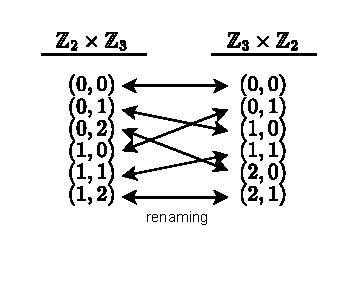
\includegraphics[width=0.5\textwidth]{Figures/IsomorphicDirectProduct1.pdf}
\end{center}
Though these are ``different" groups, they have the same structure $\therefore$ they are isomorphic to each other. We commonly say $\Z_2\times \Z_3$ and $\Z_3\times\Z_2$ are the same group ``up to isomorphism".
\end{example}

\subsection*{Rule \# 3 regarding Direct Products and Isomorphisms}
\textit{Claim:} $(G_1\times G_2)\times G_3 \underset{\theta}{\approx} G_1\times (G_2\times G_3)\approx G_1\times G_2 \times G_3$.
\begin{align}
    \theta((g_1,g_2),g_3)&=(g_1,(g_2,g_3)) \nonumber \\
    \tau(g_1,(g_2,g_3))&=(g_1,g_2,g_3) \nonumber
\end{align}
Both $\theta$ and $\tau$ are isomorphisms (bijective homomorphisms) the proof is left to the reader.

\section*{Routine Check before Exam 2}
\begin{example}
\textbf{Problem:} Write $\Z_{12}\times \Z_{16}$ as a direct product of groups of prime power order. \steezybreak\\
$\Z_{12}$ is cyclic of order $12=2^2\cdot 3$.\\
$\Z_3\times \Z_4$ has order $12$ and is cyclic, because $GCD(3,4)=1$.\\
$\therefore$ $\Z_{12}\approx \Z_3\times \Z_4$. \\
Similarly, $\Z_6 \approx \Z_2\times \Z_3$. \\
\begin{align}
    \Z_{12}\times \Z_6 &\overset{Rule\ \# 1}{\approx} (\Z_3\times \Z_4)\times \Z_6 \nonumber \\
    &\overset{Rules \ \# 1 \ \& \#2}{\approx} (\Z_3\times \Z_4)\times(\Z_2\times \Z_3) \nonumber \\
    &\overset{Rule \ \#3}{\approx} \Z_3\times \Z_4\times\Z_2\times \Z_3 \nonumber \\
    &\overset{Rule \ \#2}{\approx} \Z_2\times \Z_4\times \Z_3\times  \Z_3 \nonumber \\
    & \ \ \ \ \ \nwarrow \text{Putting the "factors" in conventional order: } 2,2^2,3,3 \nonumber
\end{align}
\end{example}

\begin{example}
Write $\Z_{20}\times \Z_{18}$ as a direct product of prime power order.

$\Z_{20}$ is cyclic of order $20=2^2\cdot 5$.
$\Z_4\times\Z_5$ has order 20 and is cyclic since $GCD(4,5)=1$
$\therefore \Z_{20}\approx \Z_4\times \Z_5$
Similarly, $\Z_{18}\approx \Z_2\times \Z_9$
\begin{align}
    \therefore \Z_{20}\times \Z_{18} &\approx (\Z_4\times \Z_5)\times \Z_{18} \ \ \ \ \text{(Rule \#1)} \nonumber \\
    &\approx (\Z_4\times \Z_5)\times (\Z_{2}\times \Z_9) \ \ \ \ \text{(Rules \#1 and \#2)} \nonumber \\
    &\approx \Z_4\times \Z_5\times \Z_{2}\times \Z_9 \ \ \ \ \text{(Rule \#3)} \nonumber \\
    &\approx \Z_2\times \Z_4\times \Z_9 \times \Z_5 \nonumber \\
    & \ \ \text{Note order: }2,2^2, 3^2, 5. \nonumber
\end{align}
\end{example}

\begin{corollary}[Corollary of Rules \#1-\#3 for Direct Products of Groups]
Any direct product of finite cyclic groups is isomorphic to a direct product of cyclic groups of prime power order. \steezybreak\\
\textit{Proof:}\\
Consider $G_1\times G_2 \times \cdots \times G_k$ Where $G_i$ is cyclic of order $n_i$. Then $G_i\approx \Z_{n_i} \ \forall \ 1\leq i \leq k$.
\begin{align}
    \therefore G_1\times G_2\times \cdots \times G_k \approx \underbrace{\Z_{n_1}\times \Z_{n_2}\times \cdots \times \Z_{n_k}}_{\text{Now proceed as in previous examples}} \nonumber
\end{align}
\end{corollary}

\textit{Question:} We know that \textit{cyclic} $\implies$ \textit{abelian}. Does \textit{abelian} $\implies$ \textit{cyclic}? \textul{No.} $\Z_2\times \Z_4$ is abelian but not cyclic since $GCD(2,4)=2\neq 1$.

\begin{example}
Suppose $G_1$ cyclic of order $8$, $G_2$ is cyclic of order $10$, and $G_3$ is cyclic of order $45$. \\ 
Then $G_1\times G_2\times G_3$ is non-cyclic of order $3600$ (but \textit{is} abelian) \\ 
$G_1\approx \Z_8$ \\
$G_2 \approx \Z_{10}$ \\
$G_3\approx \Z_{45}$
\begin{align}
    G_1\times G_2\times G_3 &\approx \Z_8\times \Z_{10}\times \Z_{45} \nonumber \\
    &\approx \Z_8\times (\Z_2\times \Z_5)\times(\Z_9\times \Z_5) \nonumber \\
    &\approx \Z_2\times \Z_8\times \Z_9\times \Z_5 \times \Z_5 \nonumber
\end{align}
\end{example}

\begin{theorem}[Fundamental Structure Theorem for Finite Abelian Groups]
Every finite abelian group is isomorphic to a direct product of cyclic groups. \steezybreak\\
The standard form of the direct product is:
\begin{align}
    \Z_{d_1}\times \Z_{d_2}\times\cdots \times \Z_{d_m} \ \ \text{ where }\ \ \ d_i|d_{i+1} \ \forall \ 1\leq i \leq m-1 \nonumber
\end{align} \steezybreak\\
Two groups $\Z_{d_1}\times \Z_{d_2}\times \cdots \times \Z_{d_m}$ and $\Z_{d_1'}\times \Z_{d_2'}\times \cdots \times \Z_{d_k'}$ are isomorphic $\iff$ $k=m$ and $d_i'=d_i \ \ \forall \ 1\leq i\leq k$. \steezybreak\\
(i.e. Finite Abelian groups are isomorphic $\iff$ they have the same standard form). \steezybreak\\

\textit{Proof:} We will hold off on proof of this for now... I need one more proof earlier in the text to make this a lot easier to pull off... I will basically use Herstein's approach from pages 109-111 of \href{https://marinazahara22.files.wordpress.com/2013/10/i-n-herstein-topics-in-algebra-2nd-edition-1975-wiley-international-editions-john-wiley-and-sons-wie-1975.pdf}{Topics in Algebra 2 Ed.} which you can read yourself if you are curious. For now, I want you to be able to use this powerful result so we can continue our exploration.
\end{theorem}
\newpage
\begin{example}
Put $G_1\times G_2\times G_3$ from the previous example in standard form.

\begin{align}
    G_1\times G_2\times G_3 &\approx \Z_2\times \Z_{2^3}\times \Z_{3^2}\times \Z_{5}\times \Z_5 \nonumber \\
    & \text{ Note there are 3 primes }(2,3,5)\text{ pick the highest power of each...} \nonumber \\
    &\approx (\Z_{2^3}\times \Z_{3^2}\times \Z_5)\times (\Z_2\times \Z_5) \nonumber \\
    &\approx \Z_{360}\times \Z_{10} \nonumber \\
    &\approx \Z_{10}\times \Z_{360} \nonumber \ \ \ \ \text{(Standard form of }G ) \\
    &\nonumber \text{note that }10|360
\end{align}
\end{example}

\begin{example}
Put $G= \Z_{50}\times \Z_{20}\times \Z_4$ in standard form
\begin{align}
    G &\approx \Z_{2\cdot 5^2}\times \Z_{2^2\cdot 5}\times \Z_{2^2} \nonumber \\
    &\overset{R1}{\approx} (\Z_2\times \Z_{5^2})\times (\Z_{2^2}\times \Z_{5})\times \Z_{2^2} \nonumber \\
    &\overset{R2\&3}{\approx}\underset{\text{highest powers of both primes}}{(\Z_{5^2}\times \Z_{2^2})}\times \underset{\text{next highest available}}{(\Z_{5}\times \Z_{2^2})}\times \underset{\text{leftovers}}{\Z_2} \nonumber \\
    &\overset{R1}{\approx} \Z_{5^2\cdot 2^2}\times \Z_{5\cdot 2^2}\times \Z_{2} \nonumber \\
    &\overset{R2}{\approx} \Z_2 \times \Z_{5\cdot 2^2}\times \Z_{5^2 \cdot 2^2} \approx \Z_2\times \Z_{20} \times \Z_{100} \nonumber
\end{align}
Note in the last line, repeated application of Rule 2 allows us to write in reverse order.
\end{example}

\begin{example}
Suppose $G$ is a finite abelian group with $G\approx G_1\times G_2\times G_3$, where
\begin{align}
    &G_1 \text{ is cyclic of order }24 \nonumber \\
    &G_2 \text{ is cyclic of order }80 \nonumber \\
    &G_3 \text{ is cyclic of order }100 \nonumber
\end{align}
Find the standard form of $G$.
\begin{align}
    G_1 &\approx \Z_{24} \nonumber \\
    G_2 &\approx \Z_{80} \nonumber \\
    G_3 &\approx \Z_{100} \nonumber
\end{align}
So
\begin{align}
  G\approx G_1\times G_2\times G_3 \approx \Z_{24}\times \Z_{80}\times \Z_{100}  \nonumber
\end{align}
Now we note that $24=2^3\cdot 3$, $80=2^4\cdot 5$, $100=2^2\cdot 5^2$ ($2,3,5$ are the primes we are dealing with). Now since $2^3$ and $3$ are relatively prime $\Z_{24}\approx \Z_{2^3}\times \Z_{3}$. By a similar argument an application of rule 1 we have
\begin{align}
    \Z_{24}\times \Z_{80} \times \Z_{100} &\approx (\Z_{2^3}\times \Z_{3})\times (\Z_{2^4}\times \Z_{5})\times (\Z_{2^2}\times \Z_{5^2}) \nonumber \\
    &\approx (\Z_{2^4}\times \Z_{3}\times \Z_{5^2})\times (\Z_{2^3}\times \Z_{5})\times \Z_{2^2} \nonumber \\
    &\approx (\Z_{2^4\cdot 3 \cdot 5^2})\times (\Z_{2^3\cdot 5})\times \Z_{2^2} \nonumber \\
    &\approx \Z_{4}\times \Z_{40} \times \Z_{1200} \nonumber
\end{align}
%Put $G=\Z_{24}\times \Z_{80}\times \Z_{100}$ in standard form:
\end{example}

\begin{example}
How many \textit{different} (i.e. non-isomorphic) abelian groups of order $81$ are there? \\
Rephrase: How many different standard forms are there for order $81$? \\
List factors of $81$ which satisfy "each factor $|$ next factor"
\begin{align}
    81 &= 3^4 \longleftrightarrow \Z_{3^4}=\Z_{81}& \nonumber \\
    &= 3^3\cdot 3 \longleftrightarrow \Z_{3}\times\Z_{27}& \nonumber \\
    &= 3^2\cdot 3^2 \longleftrightarrow \Z_{9}\times \Z_{9}& \nonumber \\
    &= 3^2\cdot 3\cdot 3 \longleftrightarrow \Z_{3}\times \Z_{3}\times \Z_{9}& \nonumber \\
    &= 3\cdot 3\cdot 3\cdot 3 \longleftrightarrow \Z_{3}\times \Z_{3}\times \Z_{3}\times \Z_{3}& \nonumber 
\end{align}
The list above consists of one representative from each isomorphism class in the set of abelian groups having order $81$. So (up to isomorphism) this is a complete list of non-isomorphic abelian groups of order $81$.
\end{example}

\begin{example}
How many non-isomorphic groups of order 49 are there?
\begin{align}
    49&=7^2=p^2 \implies \ \text{abelian} \nonumber \\
    &\therefore \text{ Structure Theorem tells all} \nonumber \\
    49&= 7^2 \ \Longleftrightarrow \Z_{49} \ \ (\text{cyclic}) \nonumber \\
    &= 7\cdot 7 \Longleftrightarrow \Z_7\times \Z_7 \ \ (7,7 \text{ not rel. prime} \implies \text{ not cyclic}) \nonumber
\end{align}
\end{example}
We can generalize the result above:
\begin{proposition} 
    There are exactly $2$ non-isomorphic structures of order $p^2$ where $p$ prime.\\ They are:
    \begin{align}
        \underset{cyclic}{\Z_{p^2}} \ \ \text{ and } \ \ \underset{non-cyclic}{\Z_{p}\times \Z_{p}} \nonumber
    \end{align}
    \textit{Proof:} Argument for last example now for arbitrary prime $p$.
\end{proposition}

\begin{example} 
\begin{enumerate}[label=\alph*.)]
    \item Write the complete list of non-isomorphic abelian groups of order $24$.
\begin{center}
    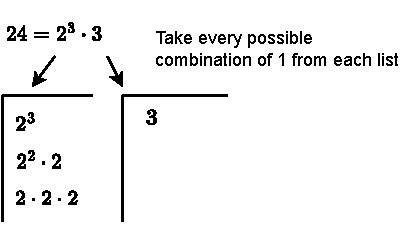
\includegraphics[width=0.55\textwidth]{Figures/24_factors.pdf}
\end{center}
\begin{align}
    \underbrace{2^3\cdot 3}_{(1)} &\longleftrightarrow \Z_{24} \ \ \ (cyclic) \nonumber \\
    \overbrace{2^2\cdot \underbrace{2}_{(2)}\cdot 3}^{(1)} &\longleftrightarrow \Z_{2}\times \Z_{12} \ \ \ (non-cyclic) \nonumber \\
    \underbrace{2\cdot \overbrace{2}^{(2)}\cdot \overbrace{2}^{(3)}\cdot 3}_{(1)} &\longleftrightarrow \Z_{2}\times \Z_2\times \Z_6 \ \ \ (non-cyclic) \nonumber 
\end{align}
\item $\Z_8\times \Z_3$ has order $24$, so it must be isomorphic to one of groups in a.)
\begin{align}
    GCD(8,3)=1 \implies \Z_8\times \Z_3 \text{ cyclic}. \nonumber
\end{align}
So $\Z_8\times \Z_3 \approx \Z_{24}$.
\item How about $\Z_6\times \Z_4$? It is order $24$ but not cyclic since $GCD(6,4)=2\neq 1$. Put $\Z_6\times \Z_4$ in standard form:
\begin{align}
    \Z_6\times \Z_4 &\approx (\Z_2\times \Z_3)\times \Z_{2^2} \nonumber \\
    &\approx \Z_2\times \Z_{12}. \nonumber
\end{align}
\end{enumerate}
\end{example}

\begin{example}
Find a representative from each of the isomorphism classes of abelian groups with order $900=2^2\cdot 3^2 \cdot 5^2$:
\begin{table}[h!]
    \centering
    \begin{tabular}{c|c|c} \hline
         $2^2$& $3^2$& $5^2$   \\ 
         $2\cdot 2$& $3\cdot 3$& $5\cdot 5$ 
    \end{tabular}
\end{table}
\begin{align}
    2^2\cdot 3^2 \cdot 5^2 &\longleftrightarrow \Z_{900} \nonumber \\
    2^2 \cdot 3^2 \cdot 5\cdot 5 &\longleftrightarrow \Z_5\times \Z_{180} \nonumber \\
    2^2 \cdot 3\cdot 3 \cdot 5^2 &\longleftrightarrow \Z_3 \times \Z_{300} \nonumber \\
    2^2 \cdot 3\cdot 3 \cdot 5 \cdot 5 &\longleftrightarrow \Z_{15} \times \Z_{60} \nonumber \\
    2\cdot 2 \cdot 3^2 \cdot 5^2 &\longleftrightarrow \Z_2\times \Z_{450} \nonumber \\
    2\cdot 2 \cdot 3^2 \cdot 5 \cdot 5  &\longleftrightarrow \Z_{10}\times \Z_{90} \nonumber \\
    2\cdot 2 \cdot 3 \cdot 3 \cdot 5^2 &\longleftrightarrow \Z_{6}\times \Z_{150} \nonumber \\
    2\cdot 2\cdot 3\cdot 3 \cdot 5 \cdot 5 &\longleftrightarrow \Z_{30}\times \Z_{30} \nonumber
\end{align}
The list above contains 8 different lattices, 1 is cyclic, the rest are non-cyclic, non-isomorphic to each other.
\end{example}
\subsection*{For Test 2:}
Know how to take orders of elements. Here are some other facts that are useful to review for this exam:
\begin{enumerate}[label=(\arabic*.)]
    \item For $p$ prime: \\ 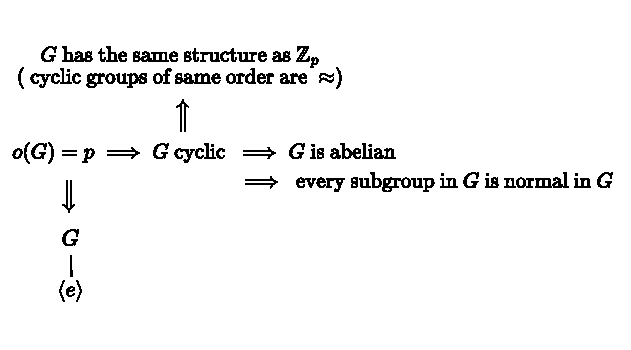
\includegraphics[width=0.65\textwidth]{Figures/prime_order_properties_1.pdf}
    \item For $p$ prime: \\
    \begin{align}
        o(G)=p^2 \implies \ G\text{ abelian }\overset{Structure Thm.}{\implies} G &\approx Z_{p^2} \ \ \ (cyclic)\nonumber \\
        \ \ \ \text{ or } \nonumber \\
        G &\approx Z_{p}\times \Z_{p} \ \ \ (non-cyclic) \nonumber
    \end{align}
    \item For primes $p,q$ where $p>q$: \\
    \begin{align}
        o(G)=pq \nonumber
    \end{align}
    Recall from class:
    \begin{align}
        o(G)=15 \implies G\text{ cyclic}\nonumber
    \end{align}
    And from HW\#8:
    \begin{align}
        o(G)=77\implies G\text{ cyclic}\nonumber
    \end{align}
    but 
    \begin{align}
        o(G)=6 \implies G &\text{ not necessarily cyclic} \nonumber \\
        &\text{could  be } \Z_6 \text{ or } D_3 \ (\text{non-abelian}\implies \text{non-cyclic}) \nonumber
    \end{align}
    In this scenario, the number of $p$-sylow subgroups is exactly 1 (Sylow \#1 $\implies $ at least one, and Cor. of Thm 2.5.1 $\implies$ at most one.) \\
    The number of $q-$Sylow subgroups $\begin{cases}
    \text{ divides }p (1 \text{ or }p)\\
    \equiv 1\mod q \ (\text{can't eliminate either})
\end{cases}$\\
Both of the above scenarios can occur. \steezybreak\\
In fact, it can be shown that if $p\not \equiv 1 \mod q$, $G$ has exactly one subgroup of order $q\ \ \implies G$ is cyclic.
\begin{align}
    o(G)=&77=7\cdot 11 \nonumber \\
    &11\equiv 4 \mod 7 \nonumber \\
    o(G)=&15= 3\cdot 5 \nonumber \\
    &5\equiv 2 \mod 3 \implies \ G \text{ cyclic} \nonumber \\
    \text{if }p \equiv 1 \mod q \implies \ G \text{ could have: }&\begin{cases}
      \text{a single } \ q-\text{Sylow subgroup } \implies G \text{ cyclic }\\
      \\
      \text{ or } \\
      \\
      p \text{ different } \ q-\text{Sylow subgroups } \implies G \text{ non-cyclic}\\ 
      \text{ and } G\approx D_p \iff q=2
    \end{cases} \nonumber
\end{align}
\end{enumerate}
Next we will take some time to review/classify the finite group structures we have looked at for various orders (up to 29 should be good enough) but first here are some useful facts:
\begin{enumerate}
    \item \begin{align}
    \text{For }p \text{ odd prime (i.e. }p\neq 2) \text{ we have that } \nonumber \\
    o(G)=p^4 \implies 5 \text{ abelian group structures and } 10 \text{ non-abelian} \nonumber
\end{align}
\item \begin{align}
    \text{For }p \text{ prime (in general) } \text{ we have that } \nonumber \\
    o(G)=p^3 \implies 3 \text{ abelian group structures and } 2 \text{ non-abelian} \nonumber
\end{align}
\end{enumerate}
\newpage 
\begin{table}[ht!]
    \centering
    \begin{tabular}{|l|p{0.75\textwidth}|} \hline
         \textbf{Order / }$o(G)$ & \textbf{Groups}  \\ \hline
         $1$ & $\langle e \rangle$ \\ \hline
         $2$ (prime) & $\Z_2$ \\  \hline
         $3$ (prime) & $\Z_3$ \\ \hline
         $4$ ($p^2\implies abelian)$ & $\Z_4 , \ \Z_2\times \Z_2$ \\ \hline
         $5$ & $\Z_5$ \\ \hline
         $6$ & $\Z_6,\ D_3\approx S_3$ \\ \hline
         $7$ & $\Z_7$ \\ \hline
         $8$ & $\Z_8, \ \Z_2\times \Z_4,  \ \Z_2\times \Z_2\times \Z_2, \ D_4, \ Q_2$ \\ \hline
         $9$ & $\Z_9, \ \Z_3\times \Z_3$ (cyclic, non-cyclic)\\ \hline
         $10$ & $\Z_{10}, \ D_5$ \\ \hline
         $11$ & $\Z_{11}$ \\ \hline
         $12=2^2\cdot 3$ & $\Z_{12}, \ \Z_2\times \Z_6, \ D_6, \ Q_3, \ A_4$ \\ \hline
         $13$ & $\Z_{13}$ \\ \hline
         $14$ & $\Z_{14}, \ D_7$ \\ \hline
         $15$ & $\Z_{15}$ \\ \hline
         $16=2^4$ & $\Z_{16}, \ \Z_2\times \Z_8,\ \Z_4\times \Z_4, \ \Z_2\times \Z_2\times \Z_4, \ \newline \Z_2\times \Z_2\times \Z_2\times \Z_2, \ D_8, \ Q_4, \ + 7$ more non-abelian \\  \hline
         $17$ & $\Z_{17}$ \\  \hline
         $18=3^2\cdot 2$ & $\Z_{18}, \ \Z_3\times \Z_6, \ D_9,  \ + 2$ more non-abelian \\ \hline
         $19$ & $\Z_{19}$ \\ \hline
         $20$ & $\Z_{20}, \ \Z_2\times \Z_{10}, \ Q_5, \ D_{10} \ + 1$ non-abelian \\ \hline
         $21=7\cdot 3, \ 7\equiv 1\mod 3$ & $\Z_{21},  \ G=\langle a,b\rangle$ \newline where $a^7=e, b^3=e, \ ba=a^2b \implies \text{ non-abelian }\implies \text{ non-cyclic}$ \\ \hline
         $22=11\cdot 2$ & $\Z_{22}, \ D_{11}$ \\ \hline
         $23$ & $\Z_{23}$ \\ \hline
         $24$ & $\Z_{24}, \ \Z_2\times \Z_{12}, \ \Z_2\times \Z_2\times \Z_6, \ D_{12}, \ Q_6 \ S_{4} \ +9$ more non-abelian \\ \hline
         $25$ & $\Z_{25}, \ \Z_5\times \Z_5$ \\ \hline
         $26$ & $\Z_{26}, \ D_{13}$ \\ \hline
         $27=3^3$ & $\Z_{27}, \ \Z_3\times \Z_9, \ \Z_3\times \Z_3\times \Z_3, + 2$ more non-abelian \\ \hline
         $28=2^2\cdot 7$ & $\Z_{28}, \ \Z_2\times \Z_{14}, \ Q_7, \ D_{14}$ \\ \hline
         $29$ & $\Z_{29}$ \\ \hline
    \end{tabular}
\end{table} \steezybreak
\newpage
\subsection*{Some Final Topics for Review for Exam 2}
Normal Subgroups -- "easy ways..." \\
Quotient Groups -- See HW $D_{12}/H$ \\
Homomorphisms/Isomorphisms
\begin{itemize}
    \item Kernel of a homomorphism ($\triangleleft$ of domain)
    \item Kernel trivial $\implies$ map is injective
    \item image of a group ($\phi(G)$) under a hom.
\end{itemize}
Commutators \\
$D_n$'s \\
$S_n$'s $\rightarrow$ order, parity
$A_n$'s $\rightarrow$ even permutations
normalizers $\leftrightarrow$ center $(Z(G)<N(a) \ \ \forall \ a \in G)$ \\
The Class Equation \\
Direct Products, in particular remember that $\Z_{n}\times \Z_{m}$ cyclic $\iff \ GCD(n,m)=1$ \\
$G$ cyclic of order $n \ \implies G\approx \Z_n$ \\ 
$Z_n$ has exactly one subgroup for each divisor of $o(G)$ \\
$d \leftrightarrow \langle 1^{n/d}\rangle$ \\
First Isomorphism Thm. \\
Cayley's Thm. \\
Sylow Thms \\
Cauchy's Thm \\
Application of class equation:
\begin{enumerate}
    \item if $o(G)=p^m$, then $\{e\} \subsetneq Z(G)$ (there is a non-trivial element that commutes with everything)
    \item $o(G)=p^2 \ \implies G$ is abelian.
\end{enumerate}
Cyclic $\implies$ abelian\\
Abelian $\not \Rightarrow$ Cyclic  ($\Z_2\times \Z_4$ is abelian but not cyclic)\\
$A_4$ order is $12$ but has no subgroup of order $6$...


